\section{Appendix}

\subsection{Full BipedalWalker Ranking}

Table~\ref{tab:bw-full-ranking} lists all 15 BipedalWalker configurations that were trained and evaluated (50 greedy evaluation episodes each), extending the top-5 excerpt in Table~\ref{tab:overall-ranking}.

\begin{table*}[h]
    \centering
    \footnotesize
    \caption{BipedalWalker: All 15 Configurations, Ranked by Mean Return}
    \label{tab:bw-full-ranking}
    \begin{tabular}{rlrrrrr}
        \toprule
        Rank & Configuration & Policy & Mean Ret. & Std. & Median & Mean Len. \\
        \midrule
        1  & \texttt{bw\_boltzmann\_final\_01\_seed42}                        & Boltzmann      & \textbf{329.16} & 49.99 & 321.32 & 143.38 \\
        2  & \texttt{bw\_final\_02\_balanced\_replay\_explore\_400\_seed42}   & $\epsilon$-greedy & 243.00 & 50.80 & 229.60 & 132.00 \\
        3  & \texttt{bw\_03\_more\_exploration\_large\_300}                   & $\epsilon$-greedy & 163.71 & 12.57 & 164.61 & 89.52 \\
        4  & \texttt{bw\_boltzmann\_04\_more\_exploration\_temp010\_300\_seed24} & Boltzmann   & 160.57 & 14.96 & 159.09 & 88.98 \\
        5  & \texttt{bw\_01\_baseline\_large\_300}                            & $\epsilon$-greedy & 158.65 & 16.78 & 154.96 & 89.10 \\
        6  & \texttt{bw\_05\_big\_replay\_batch\_300}                         & $\epsilon$-greedy & 152.7  & 11.0  & 156.6  & 85.1 \\
        7  & \texttt{bw\_final\_03\_compromise\_explore\_long\_500\_seed13}   & $\epsilon$-greedy & 153.1  & 14.8  & 156.7  & 78.4 \\
        8  & \texttt{bw\_boltzmann\_03\_fast\_lr\_temp015\_300\_seed23}       & Boltzmann      & 146.6  & 7.3   & 146.0  & 85.6 \\
        9  & \texttt{bw\_06\_boltzmann\_large\_300}                           & Boltzmann      & 145.10 & 12.91 & 141.4  & 83.4 \\
        10 & \texttt{bw\_02\_stable\_low\_lr\_large\_300}                     & $\epsilon$-greedy & 141.3  & 13.8  & 139.8  & 82.7 \\
        11 & \texttt{bw\_final\_01\_more\_exploration\_extended\_400\_seed11} & $\epsilon$-greedy & 134.2  & 14.5  & 130.1  & 76.6 \\
        12 & \texttt{bw\_04\_medium\_network\_300}                            & $\epsilon$-greedy & 132.8  & 9.4   & 132.7  & 74.4 \\
        13 & \texttt{bw\_boltzmann\_02\_gamma995\_temp015\_250\_seed21}       & Boltzmann      & 130.5  & 30.0  & 132.2  & 82.5 \\
        14 & \texttt{bw\_boltzmann\_01\_temp15\_temp015\_250\_seed22}         & Boltzmann      & 117.1  & 19.7  & 111.1  & 79.4 \\
        15 & \texttt{bw\_07\_gamma\_097\_ablation\_300}                       & $\epsilon$-greedy & 93.41  & 33.83 & 78.7   & 70.4 \\
        \bottomrule
    \end{tabular}
\end{table*}

\subsection{Full CartPole Ranking}

Table~\ref{tab:cartpole-ranking} in Section~\ref{sec:evaluation} already lists all 10 trained CartPole-v1 configurations (100 greedy evaluation episodes each), so no additional appendix table is required.

\clearpage
\subsection{Training Curves}

All training-curve plots (reward, episode length, loss) referenced in Section~\ref{sec:evaluation} are collected below: the two headline "success case" runs (Figure~\ref{fig:bw-success}, Figure~\ref{fig:cp-success}), the six BipedalWalker ablation categories underlying Table~\ref{tab:bw-full-ranking} (Figures~\ref{fig:cat01}--\ref{fig:cat06}), and the BipedalWalker vs.\ Hardcore comparison (Figure~\ref{fig:hardcore}).

% BW success curves
\begin{figure}[H]
    \centering
    \begin{subfigure}{0.31\textwidth}
        \centering
        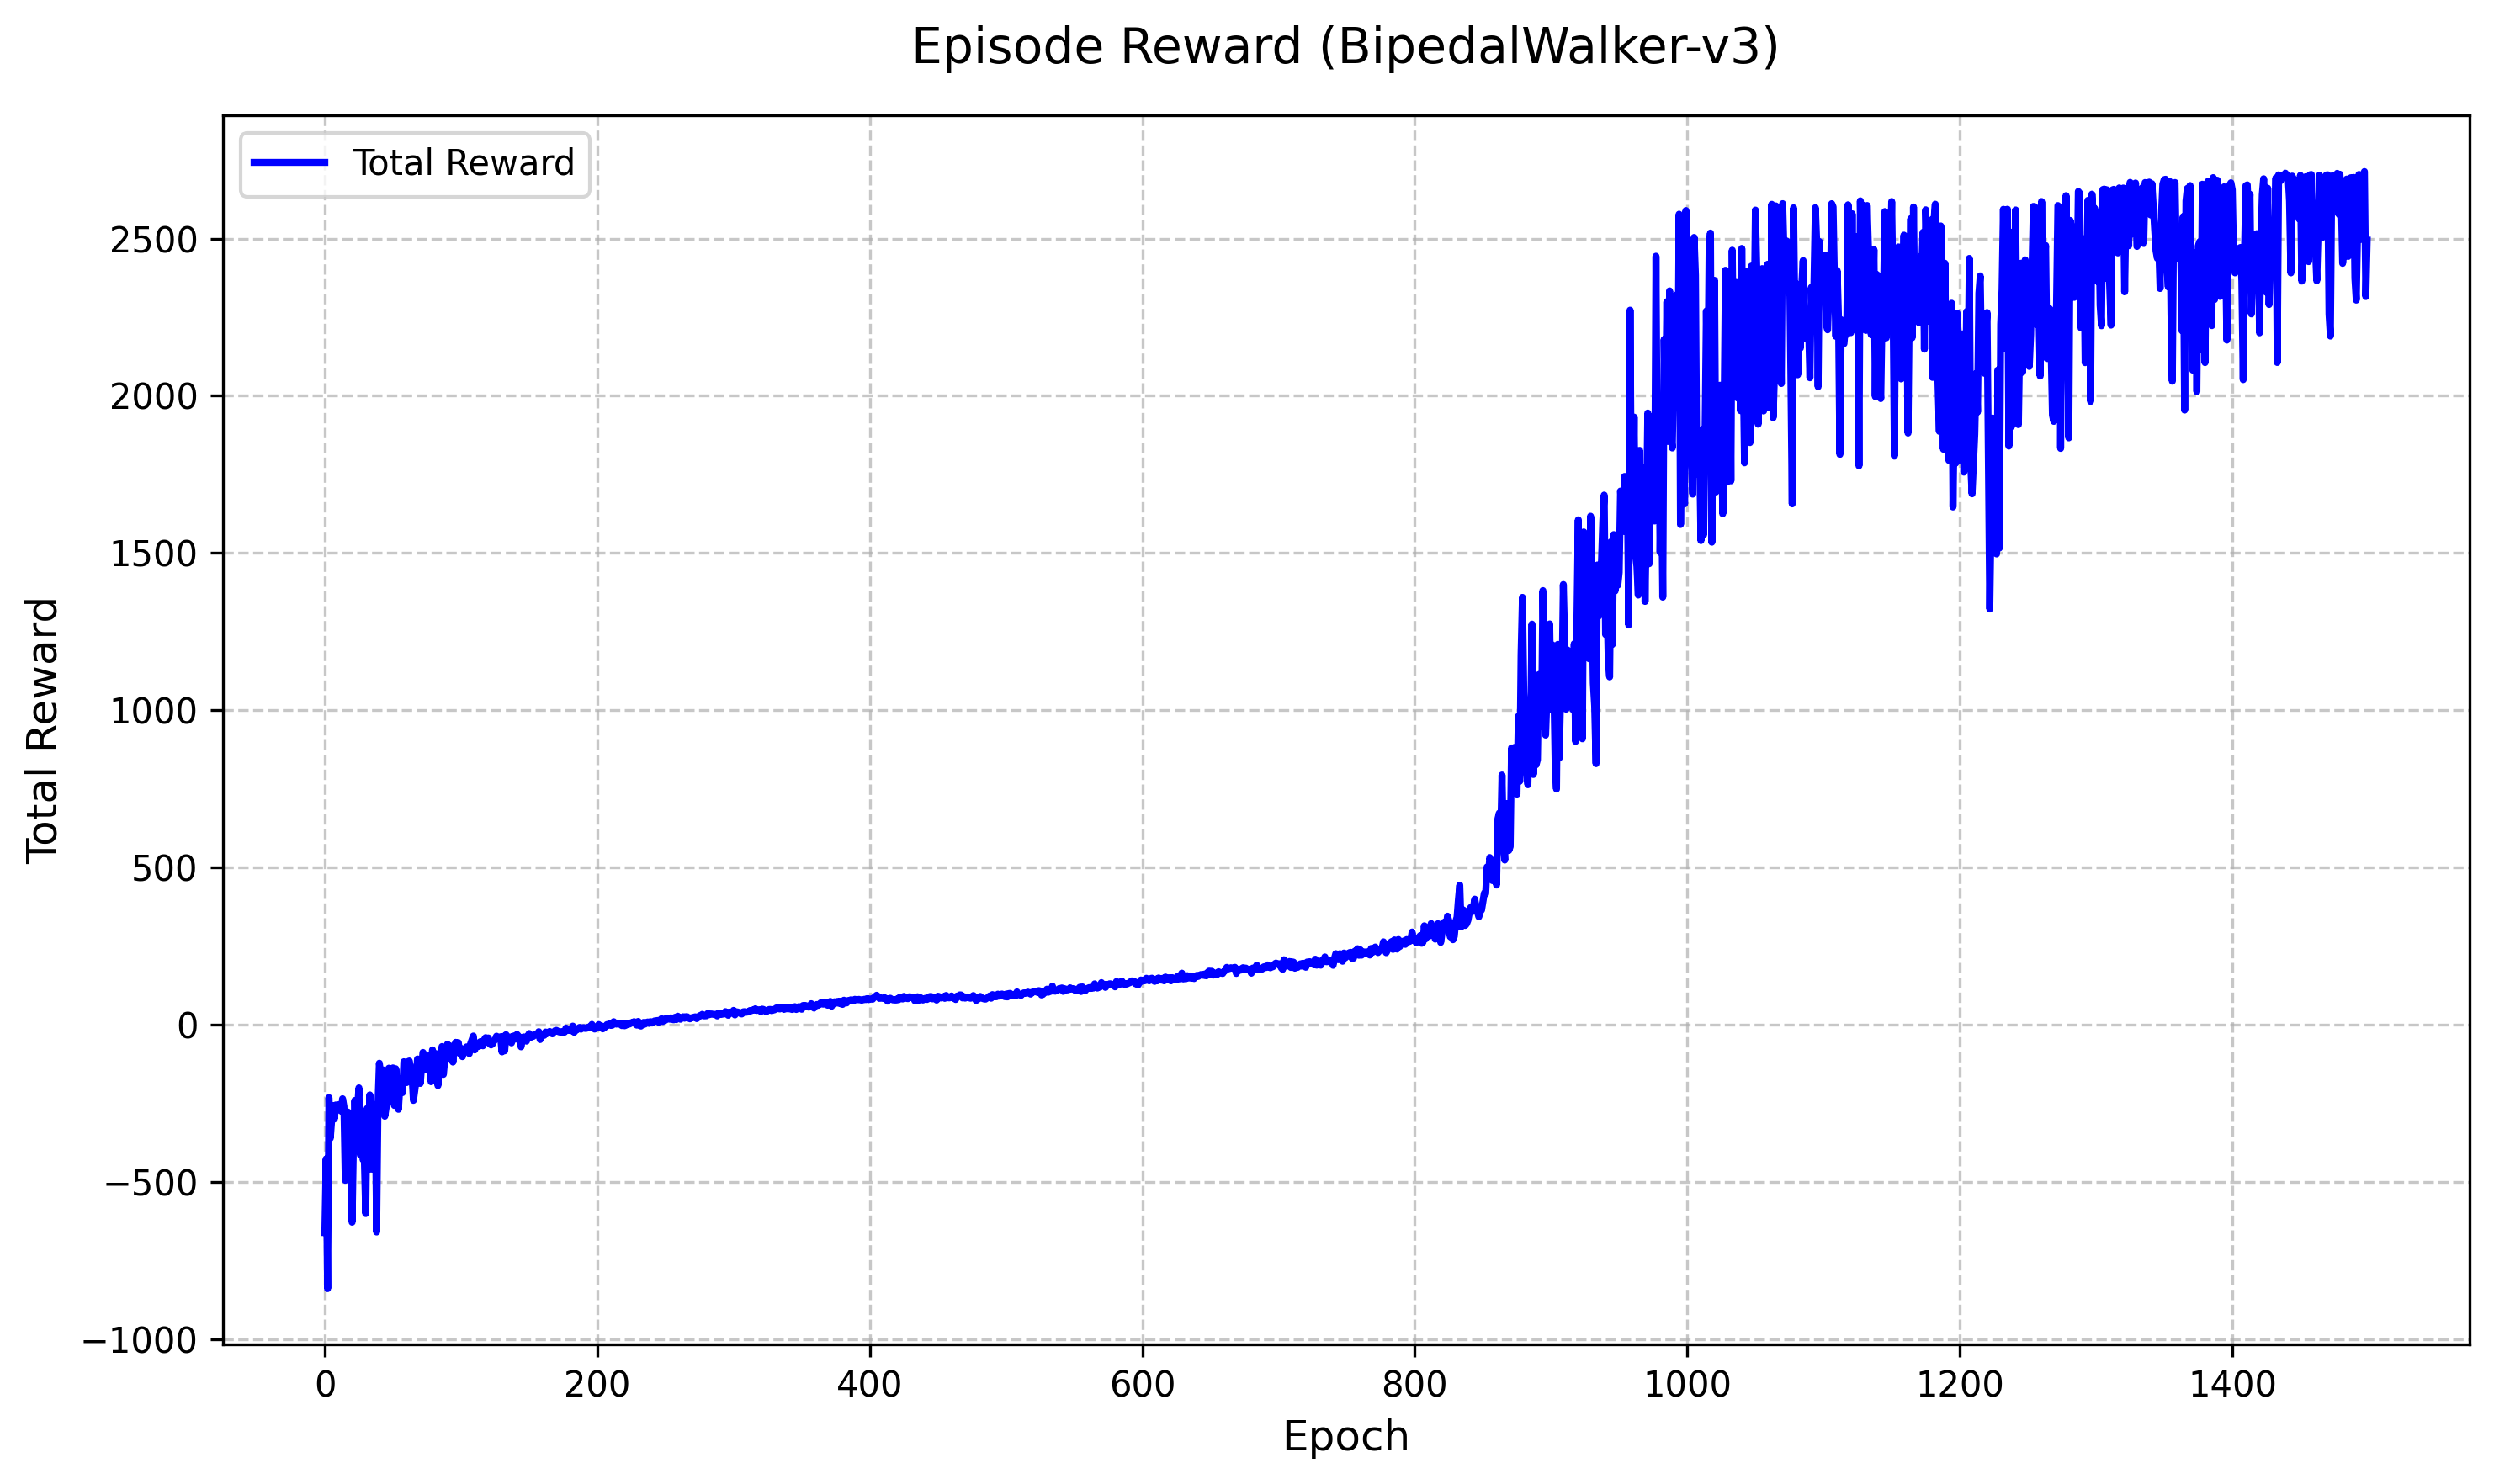
\includegraphics[width=\linewidth]{img/bw-success-reward.png}
        \caption{Reward}
    \end{subfigure}\hfill
    \begin{subfigure}{0.31\textwidth}
        \centering
        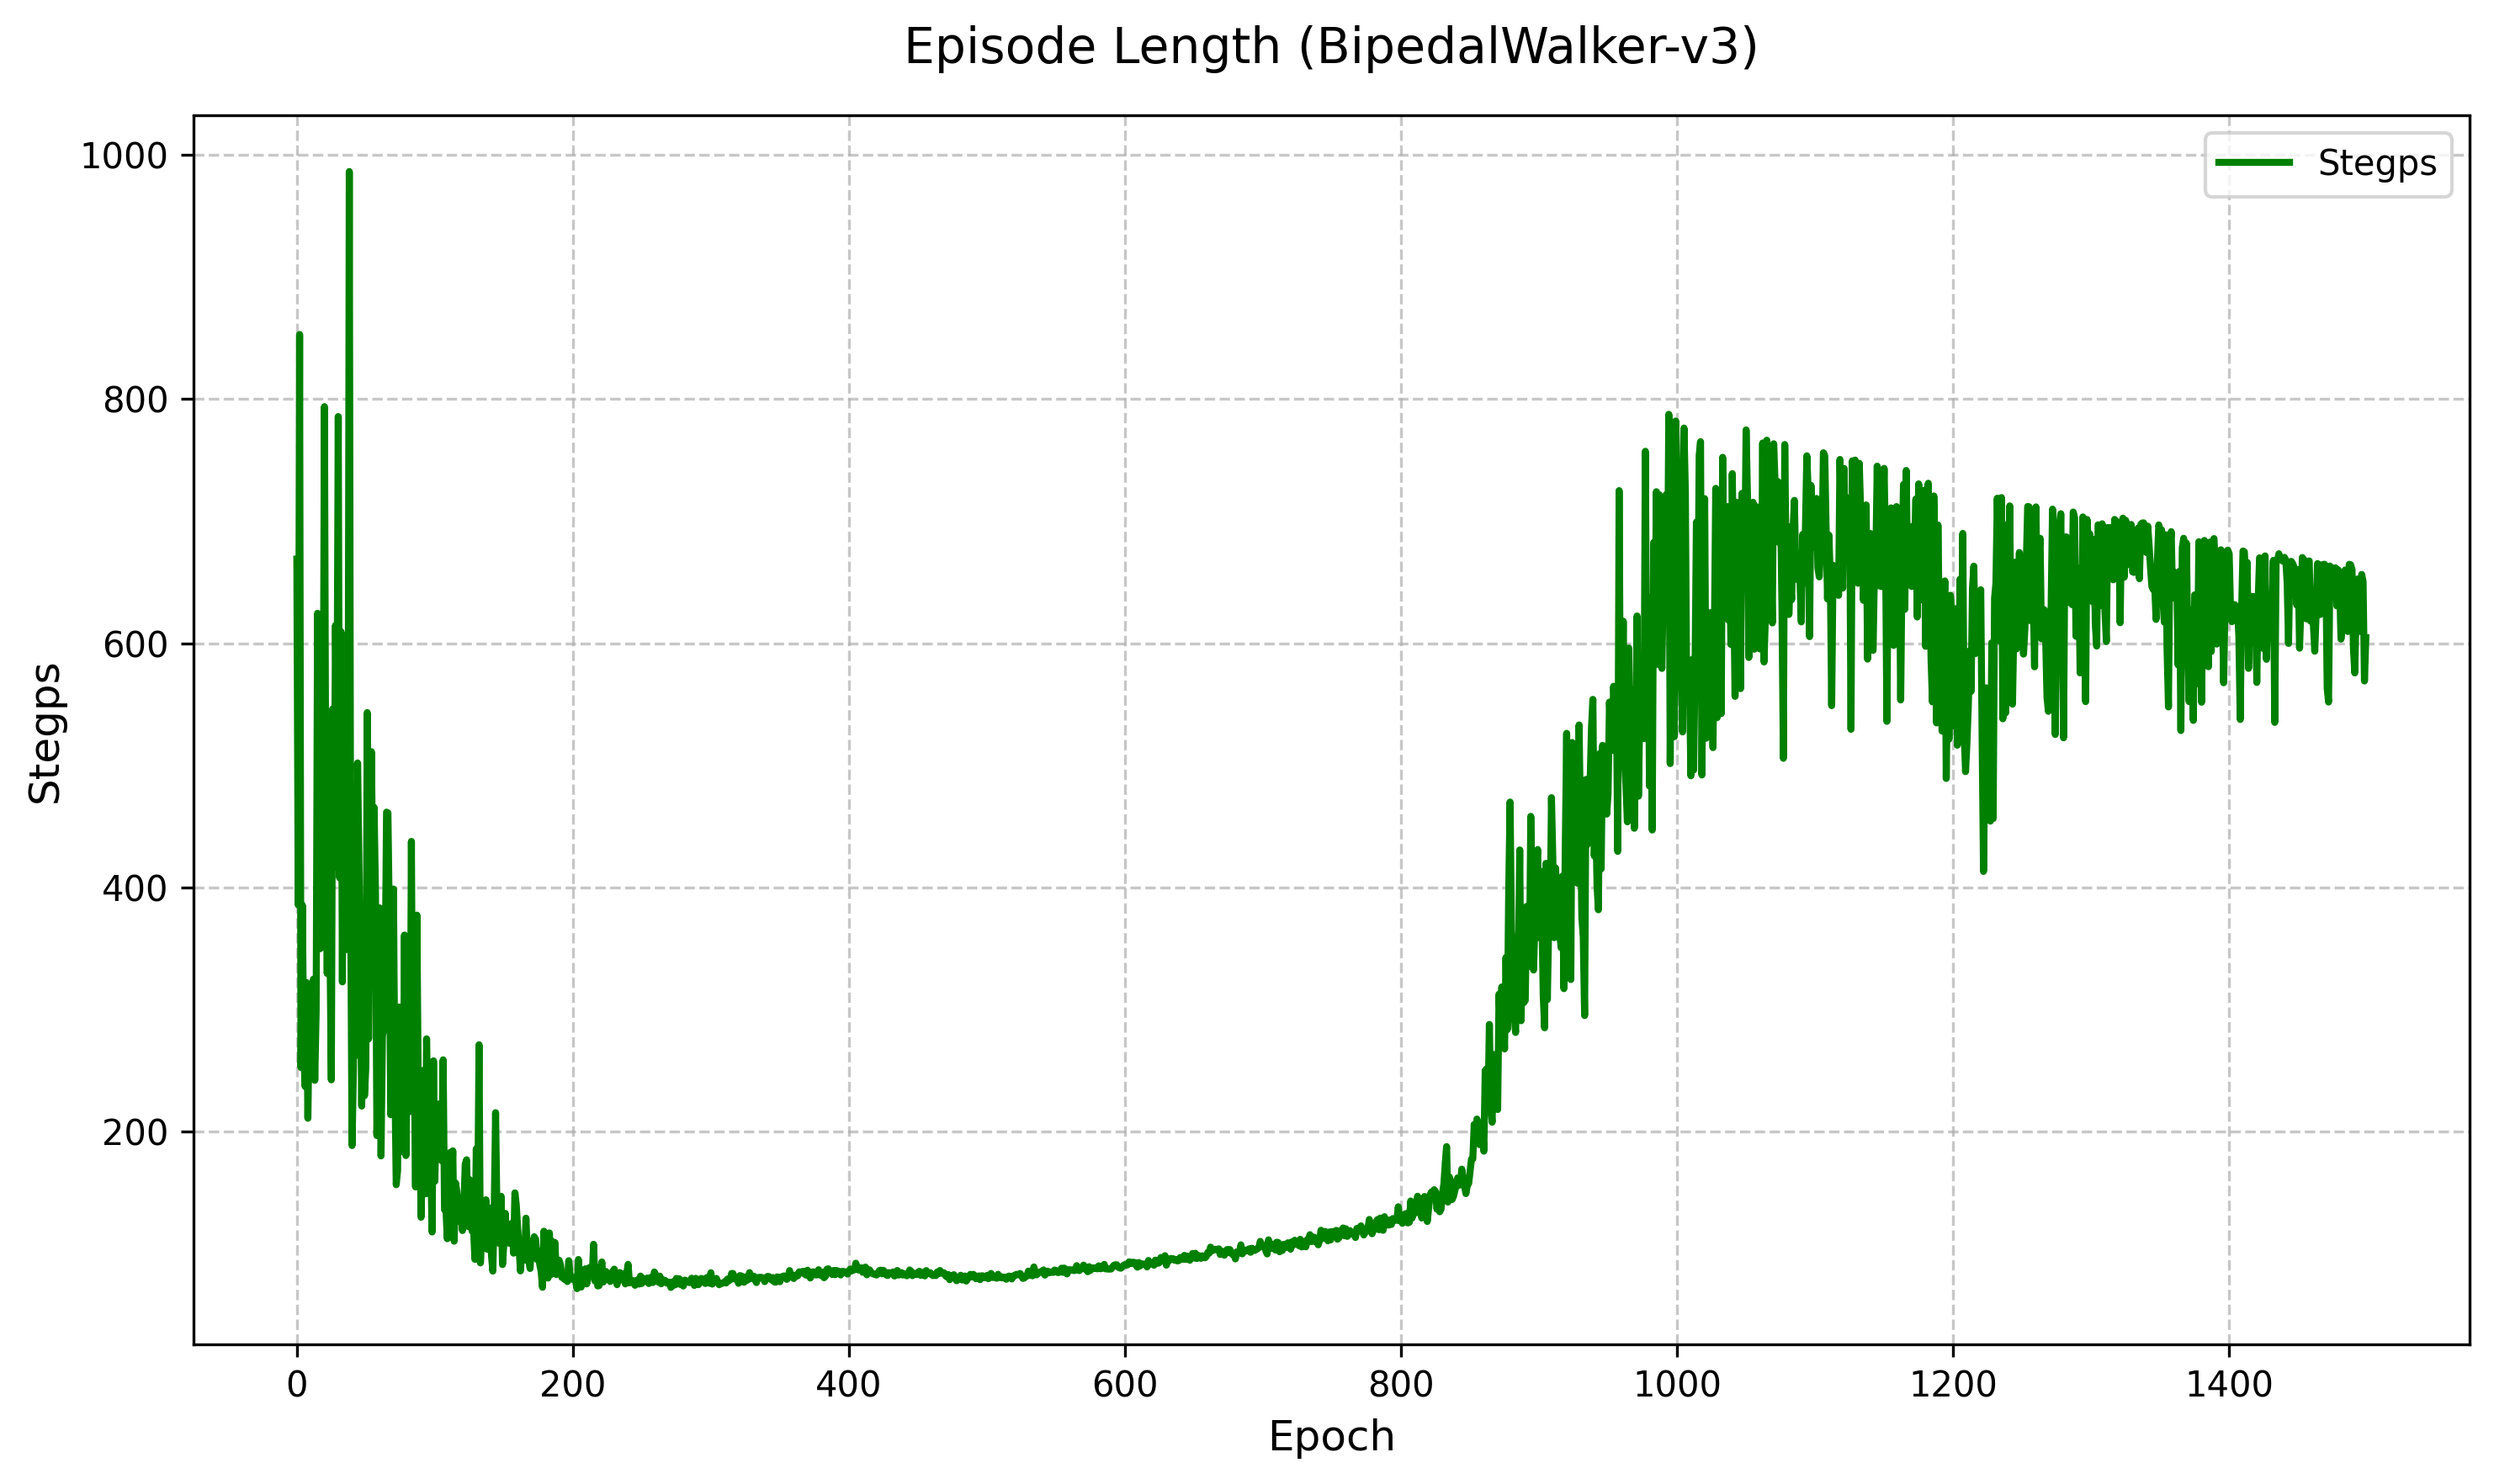
\includegraphics[width=\linewidth]{img/bw-success-length.png}
        \caption{Length}
    \end{subfigure}\hfill
    \begin{subfigure}{0.31\textwidth}
        \centering
        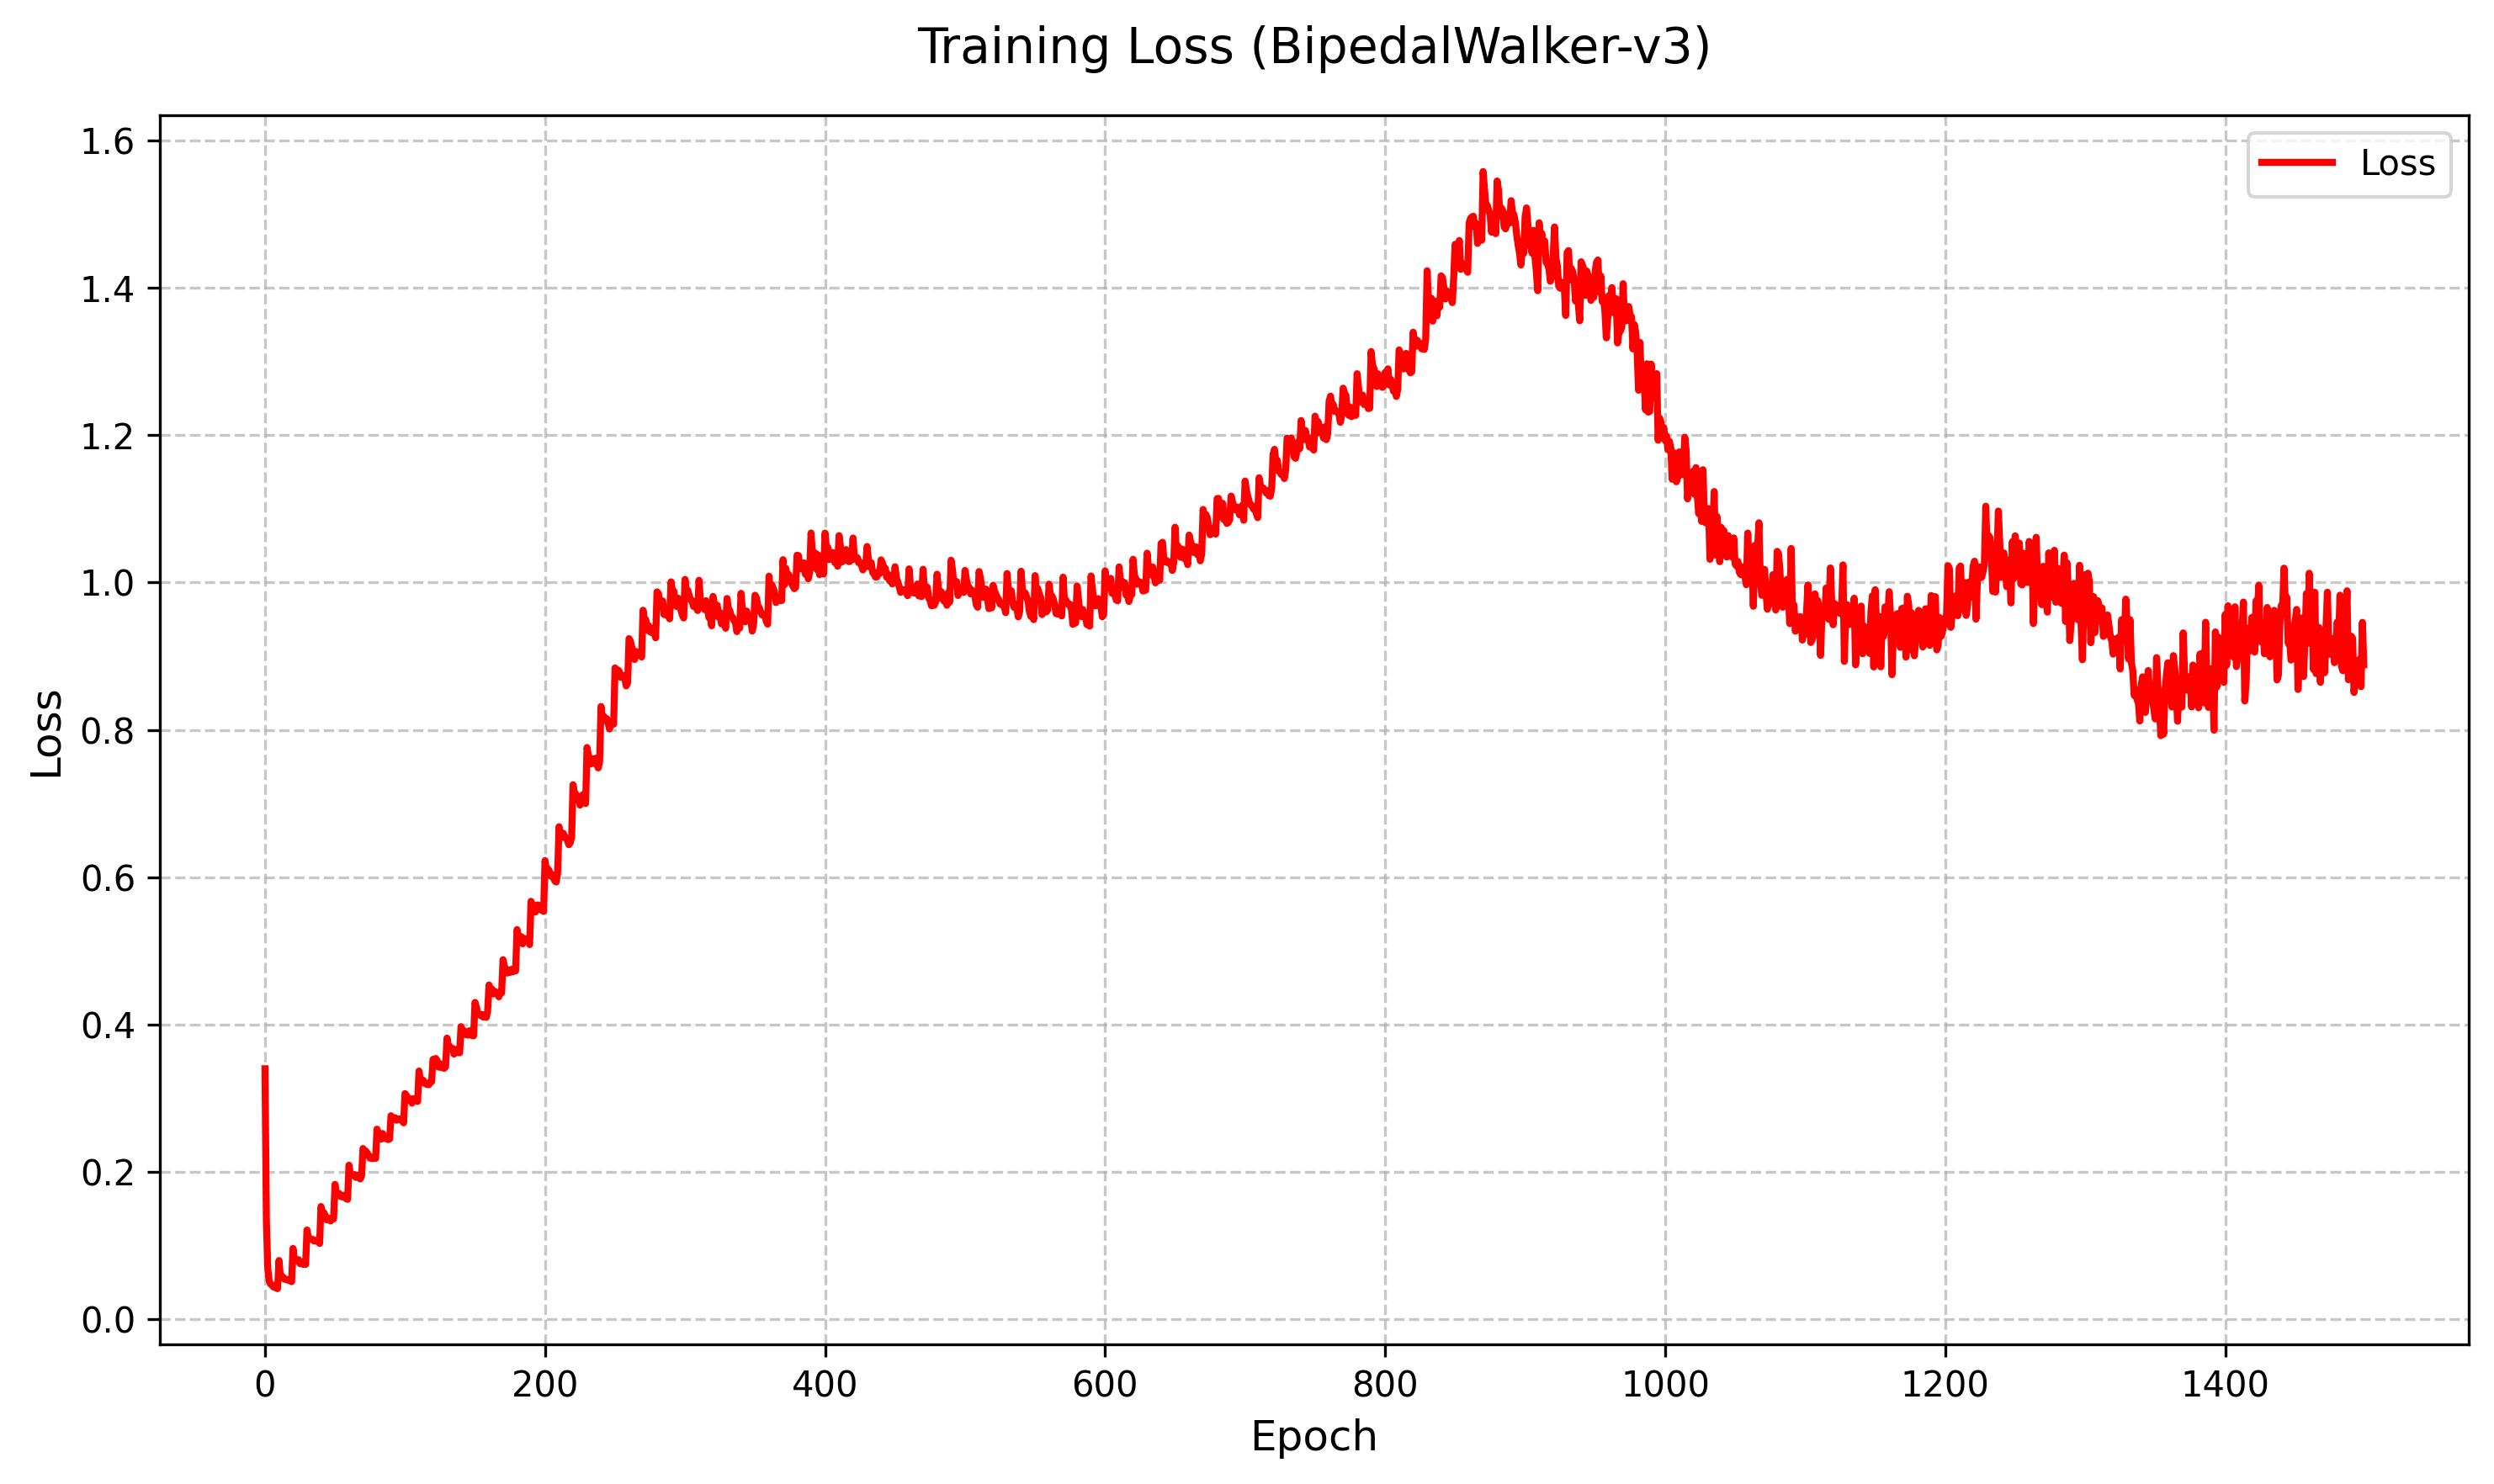
\includegraphics[width=\linewidth]{img/bw-success-loss.png}
        \caption{Loss}
    \end{subfigure}
    \caption{Best BipedalWalker configuration (\texttt{bw\_boltzmann\_final\_01\_seed42}): a long plateau followed by an abrupt rise in reward and episode length as loss decreases.}
    \label{fig:bw-success}
\end{figure}

% CartPole success curves
\begin{figure}[H]
    \centering
    \begin{subfigure}{0.31\textwidth}
        \centering
        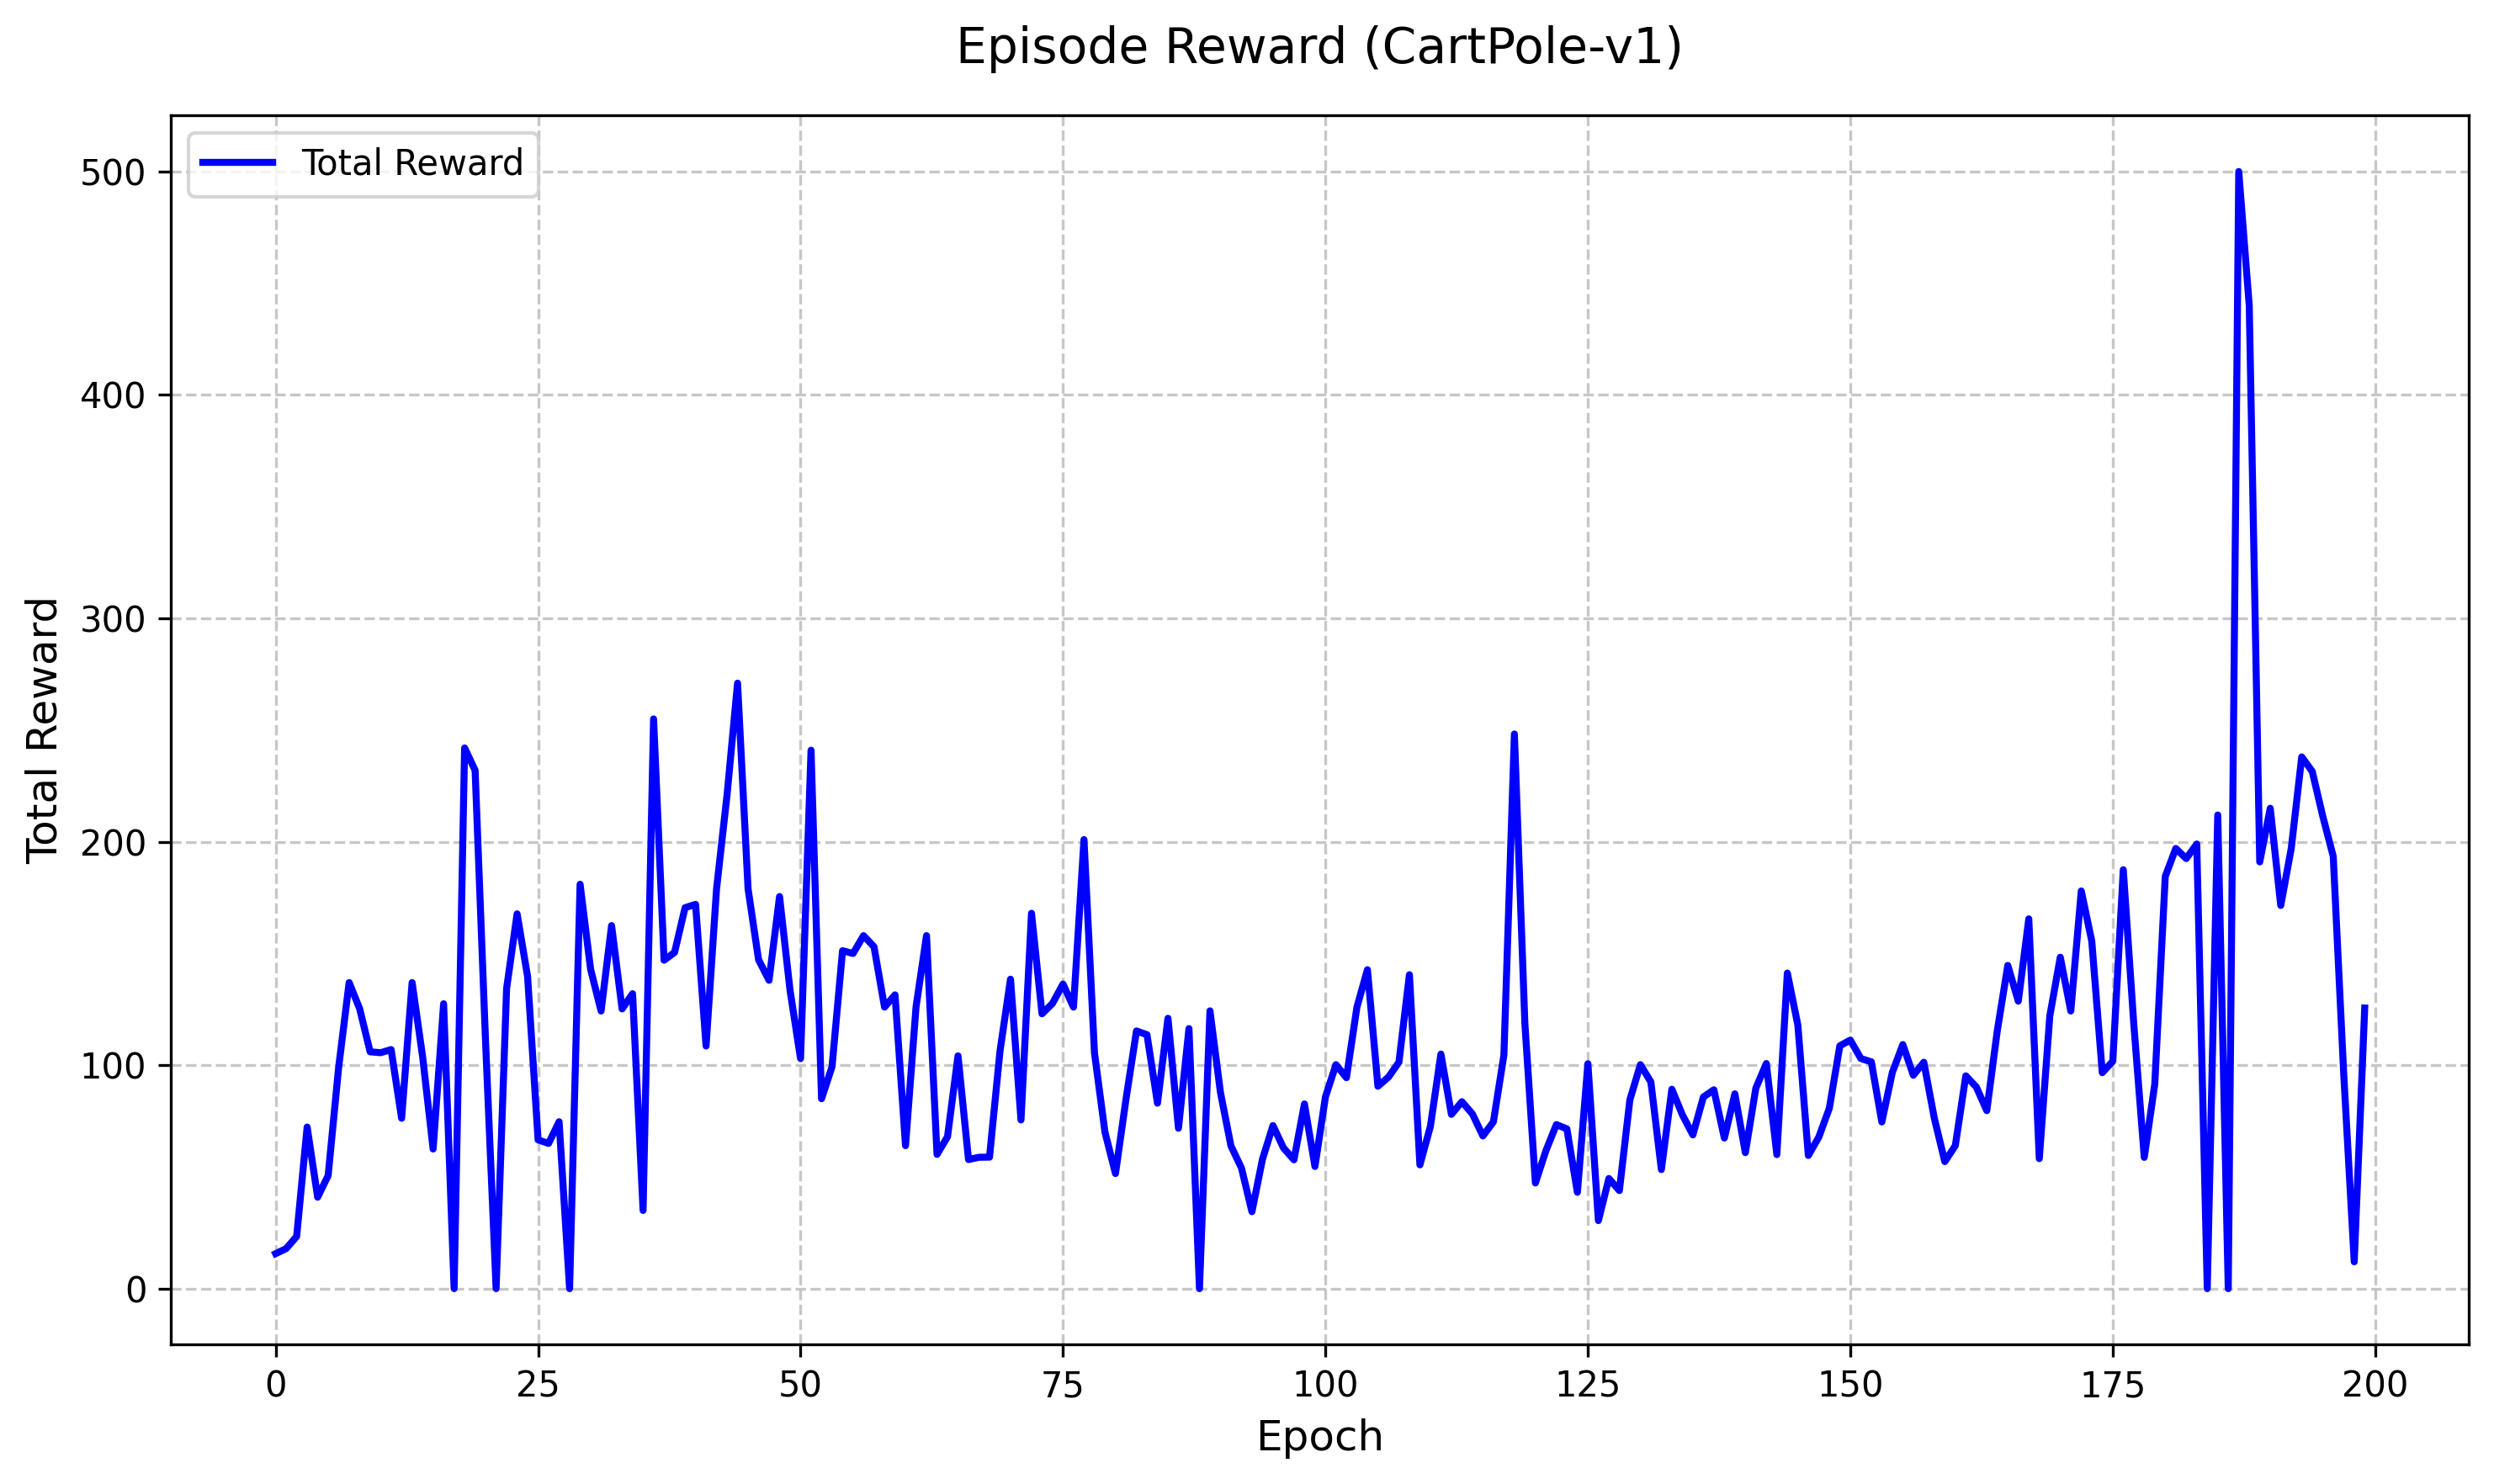
\includegraphics[width=\linewidth]{img/cp-success-epsilon-reward.png}
        \caption{Reward}
    \end{subfigure}\hfill
    \begin{subfigure}{0.31\textwidth}
        \centering
        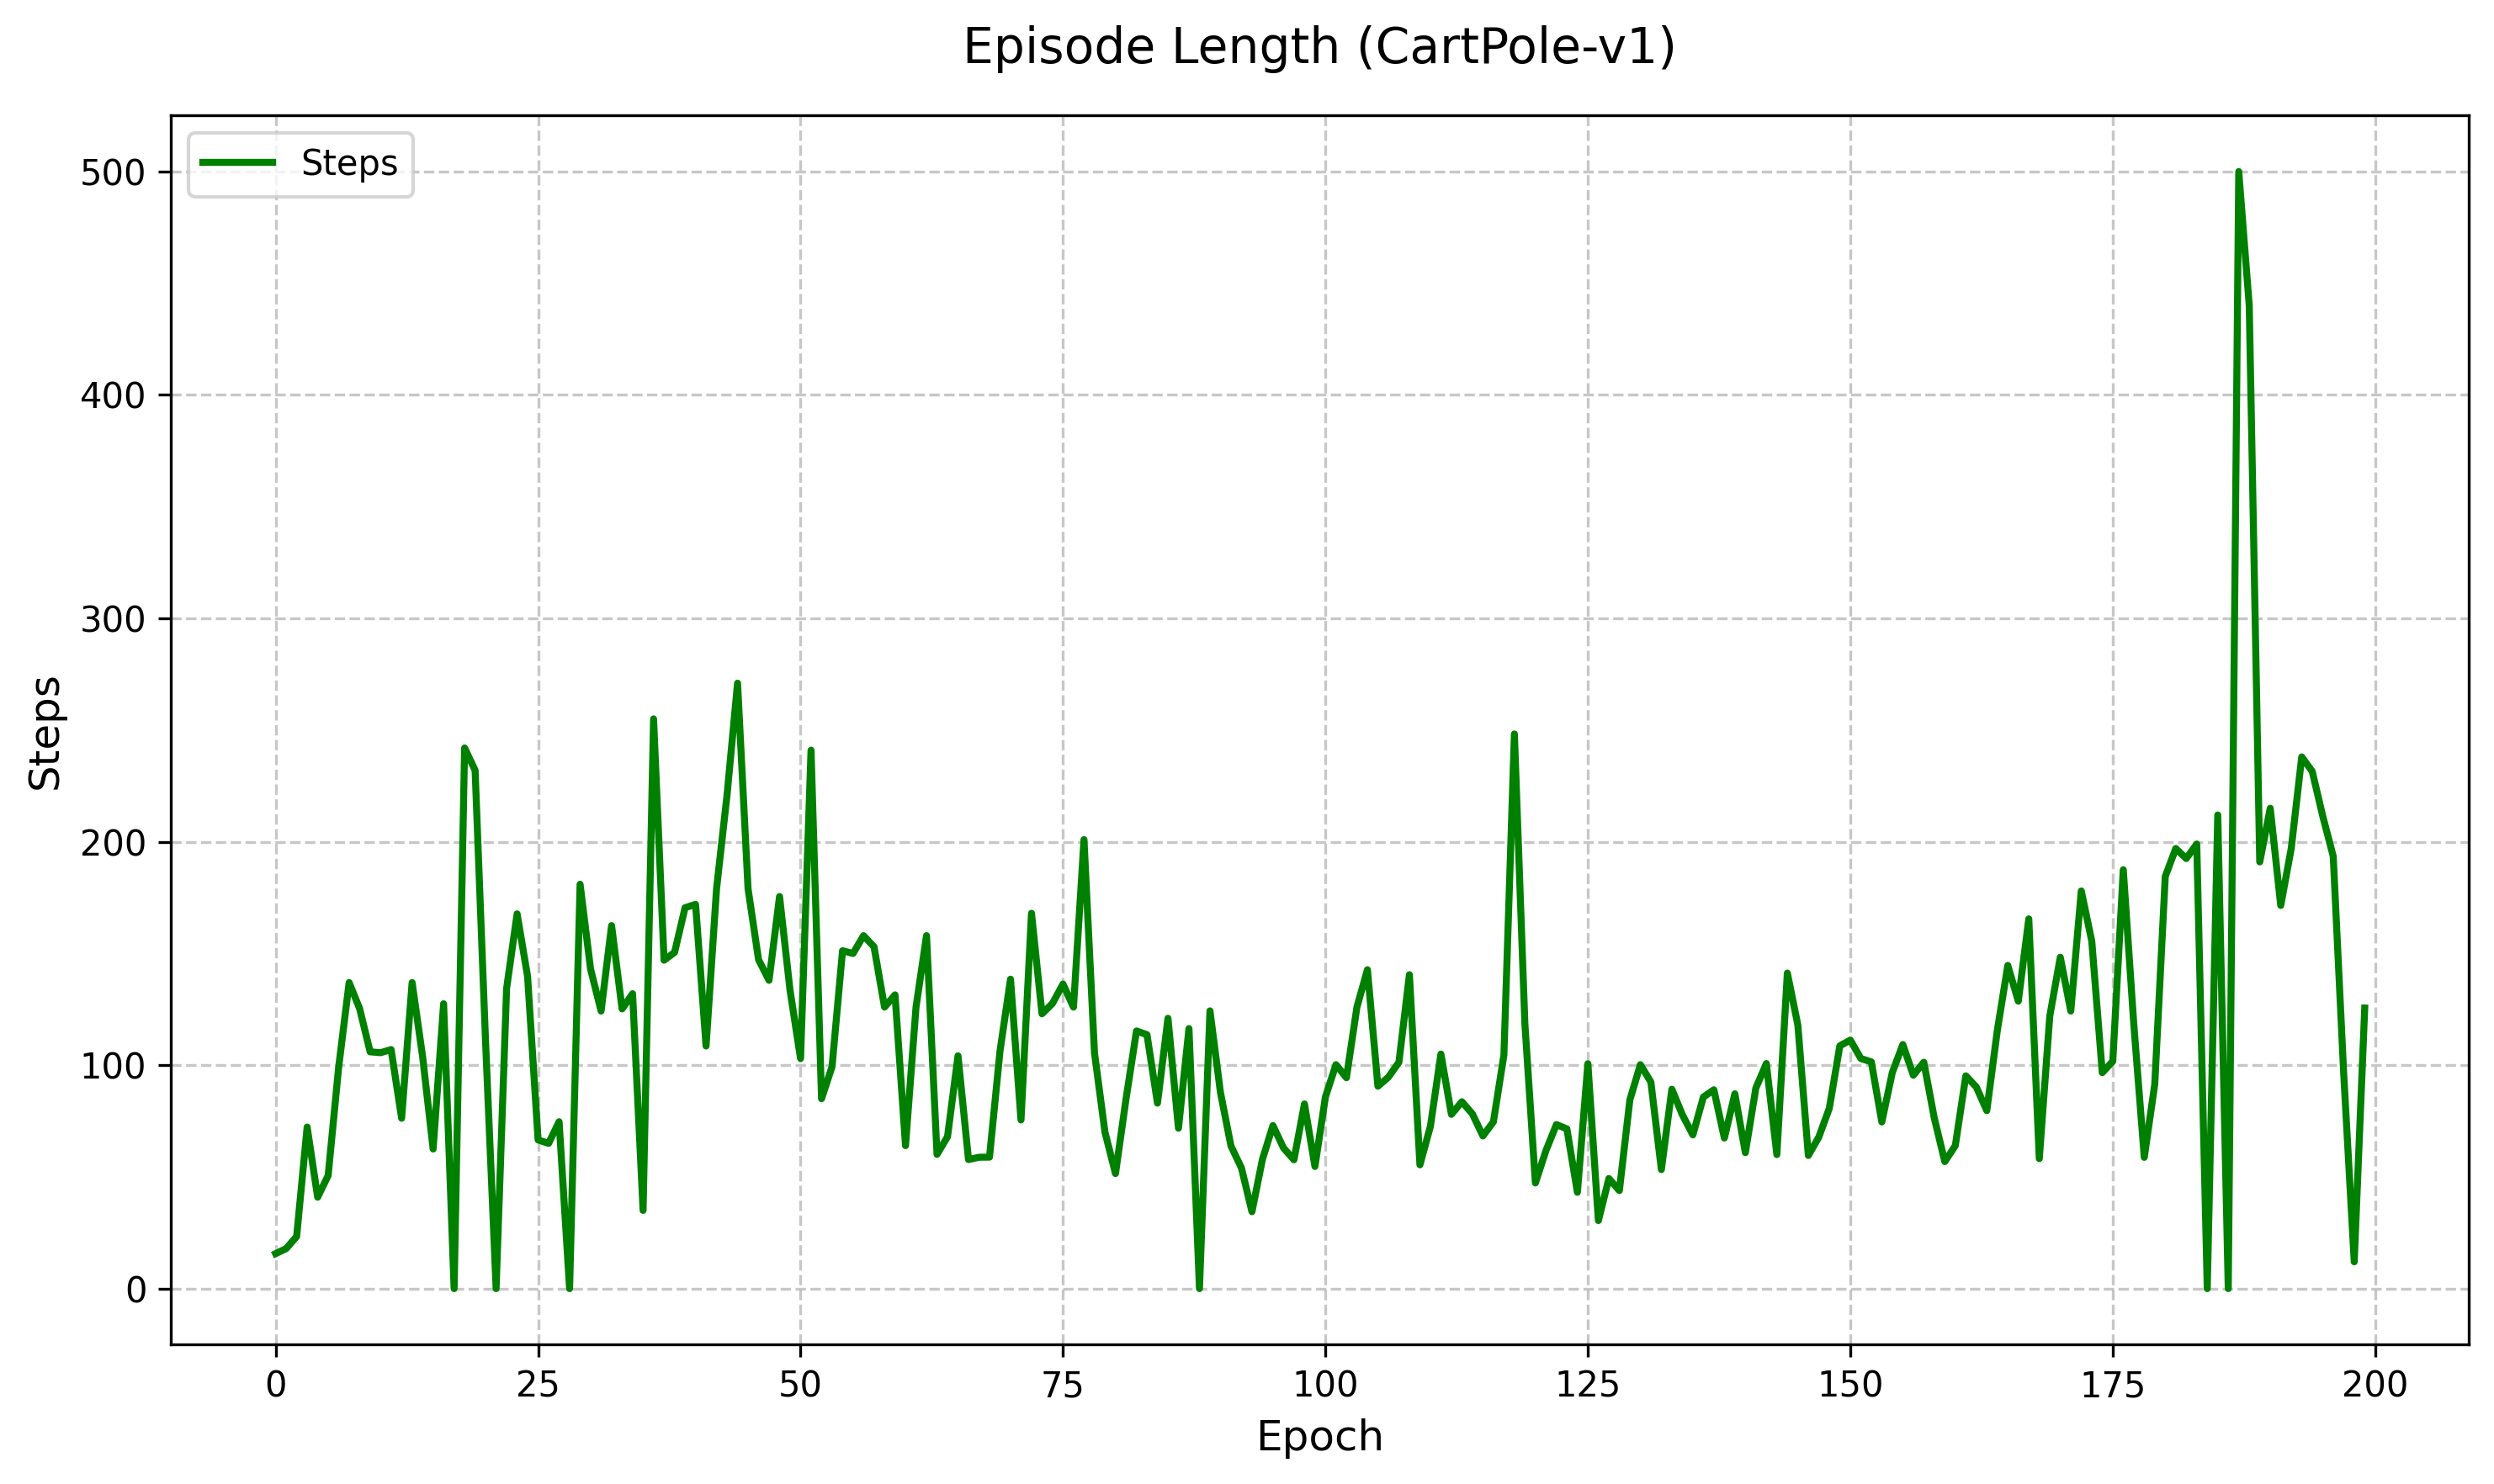
\includegraphics[width=\linewidth]{img/cp-success-epsilon-length.png}
        \caption{Length}
    \end{subfigure}\hfill
    \begin{subfigure}{0.31\textwidth}
        \centering
        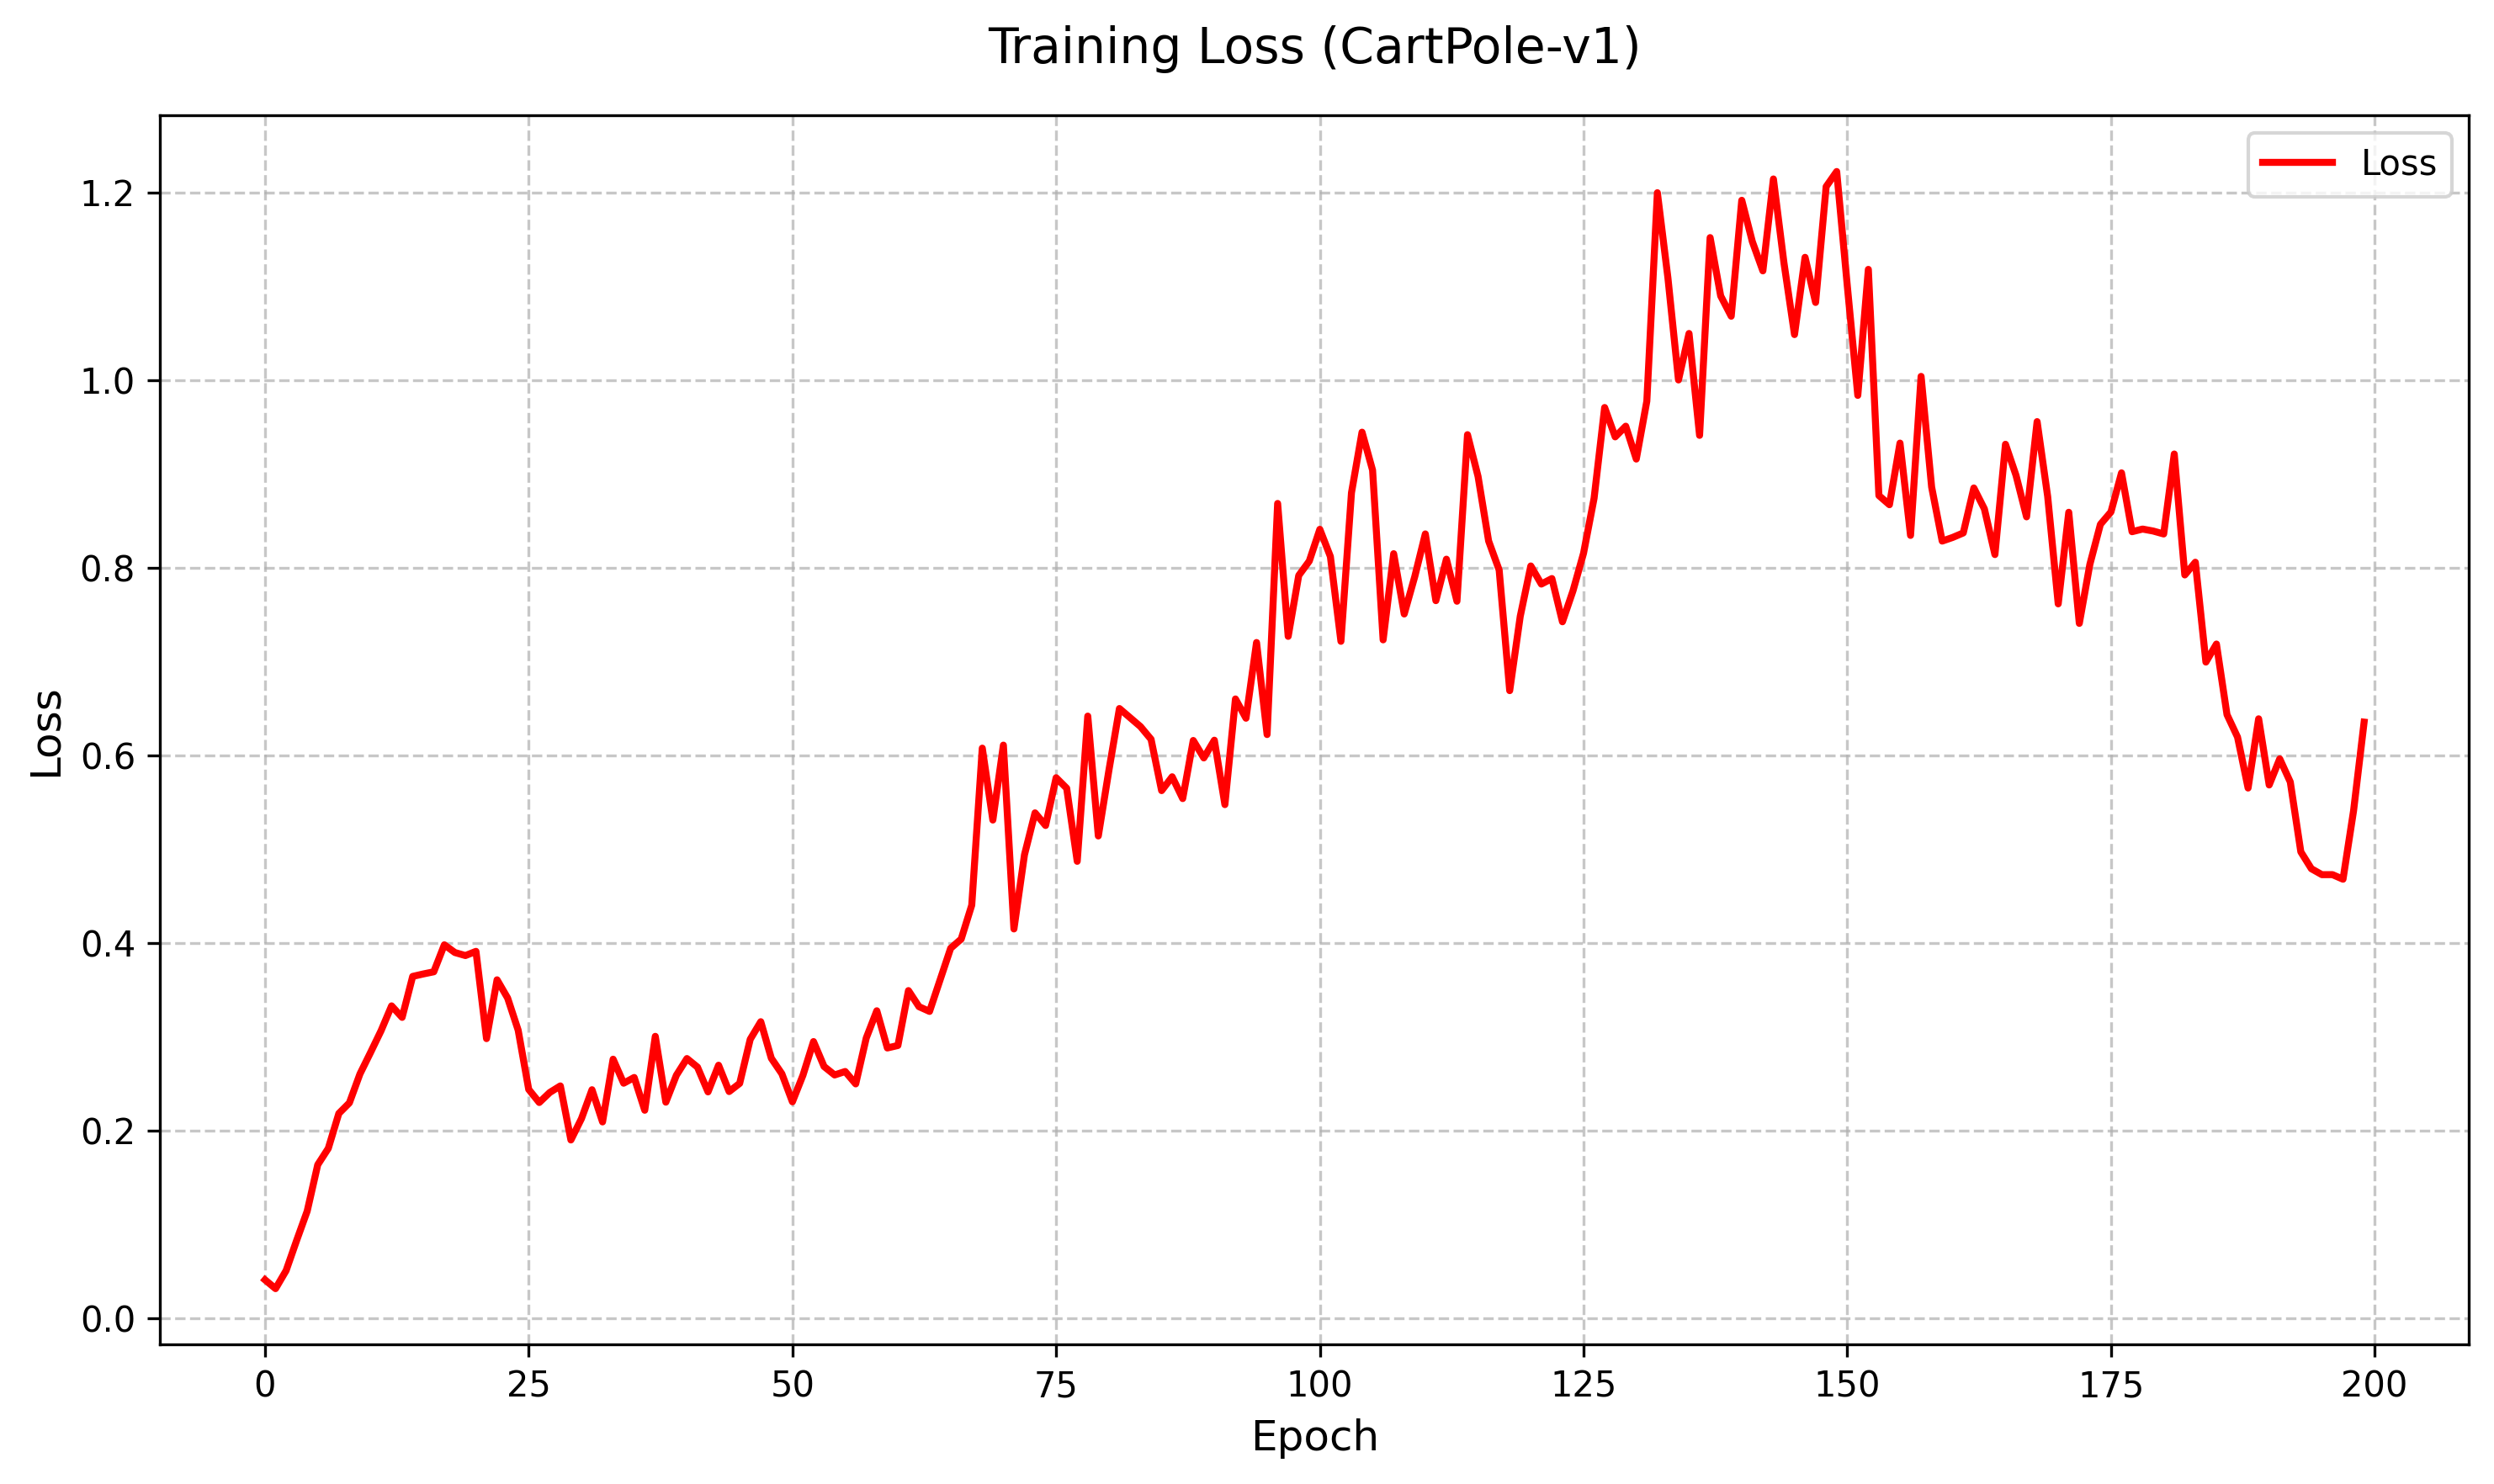
\includegraphics[width=\linewidth]{img/cp-success-epsilon-loss.png}
        \caption{Loss}
    \end{subfigure}
    \caption{Best CartPole configuration (\texttt{cp\_policy\_epsilon\_greedy}, \texttt{mlp\_small} + $\epsilon$-greedy), reaching the maximum episode length of 500.}
    \label{fig:cp-success}
\end{figure}

% 01 - Baseline vs Exploration
\begin{figure}[H]
    \centering
    \begin{subfigure}{0.31\textwidth}
        \centering
        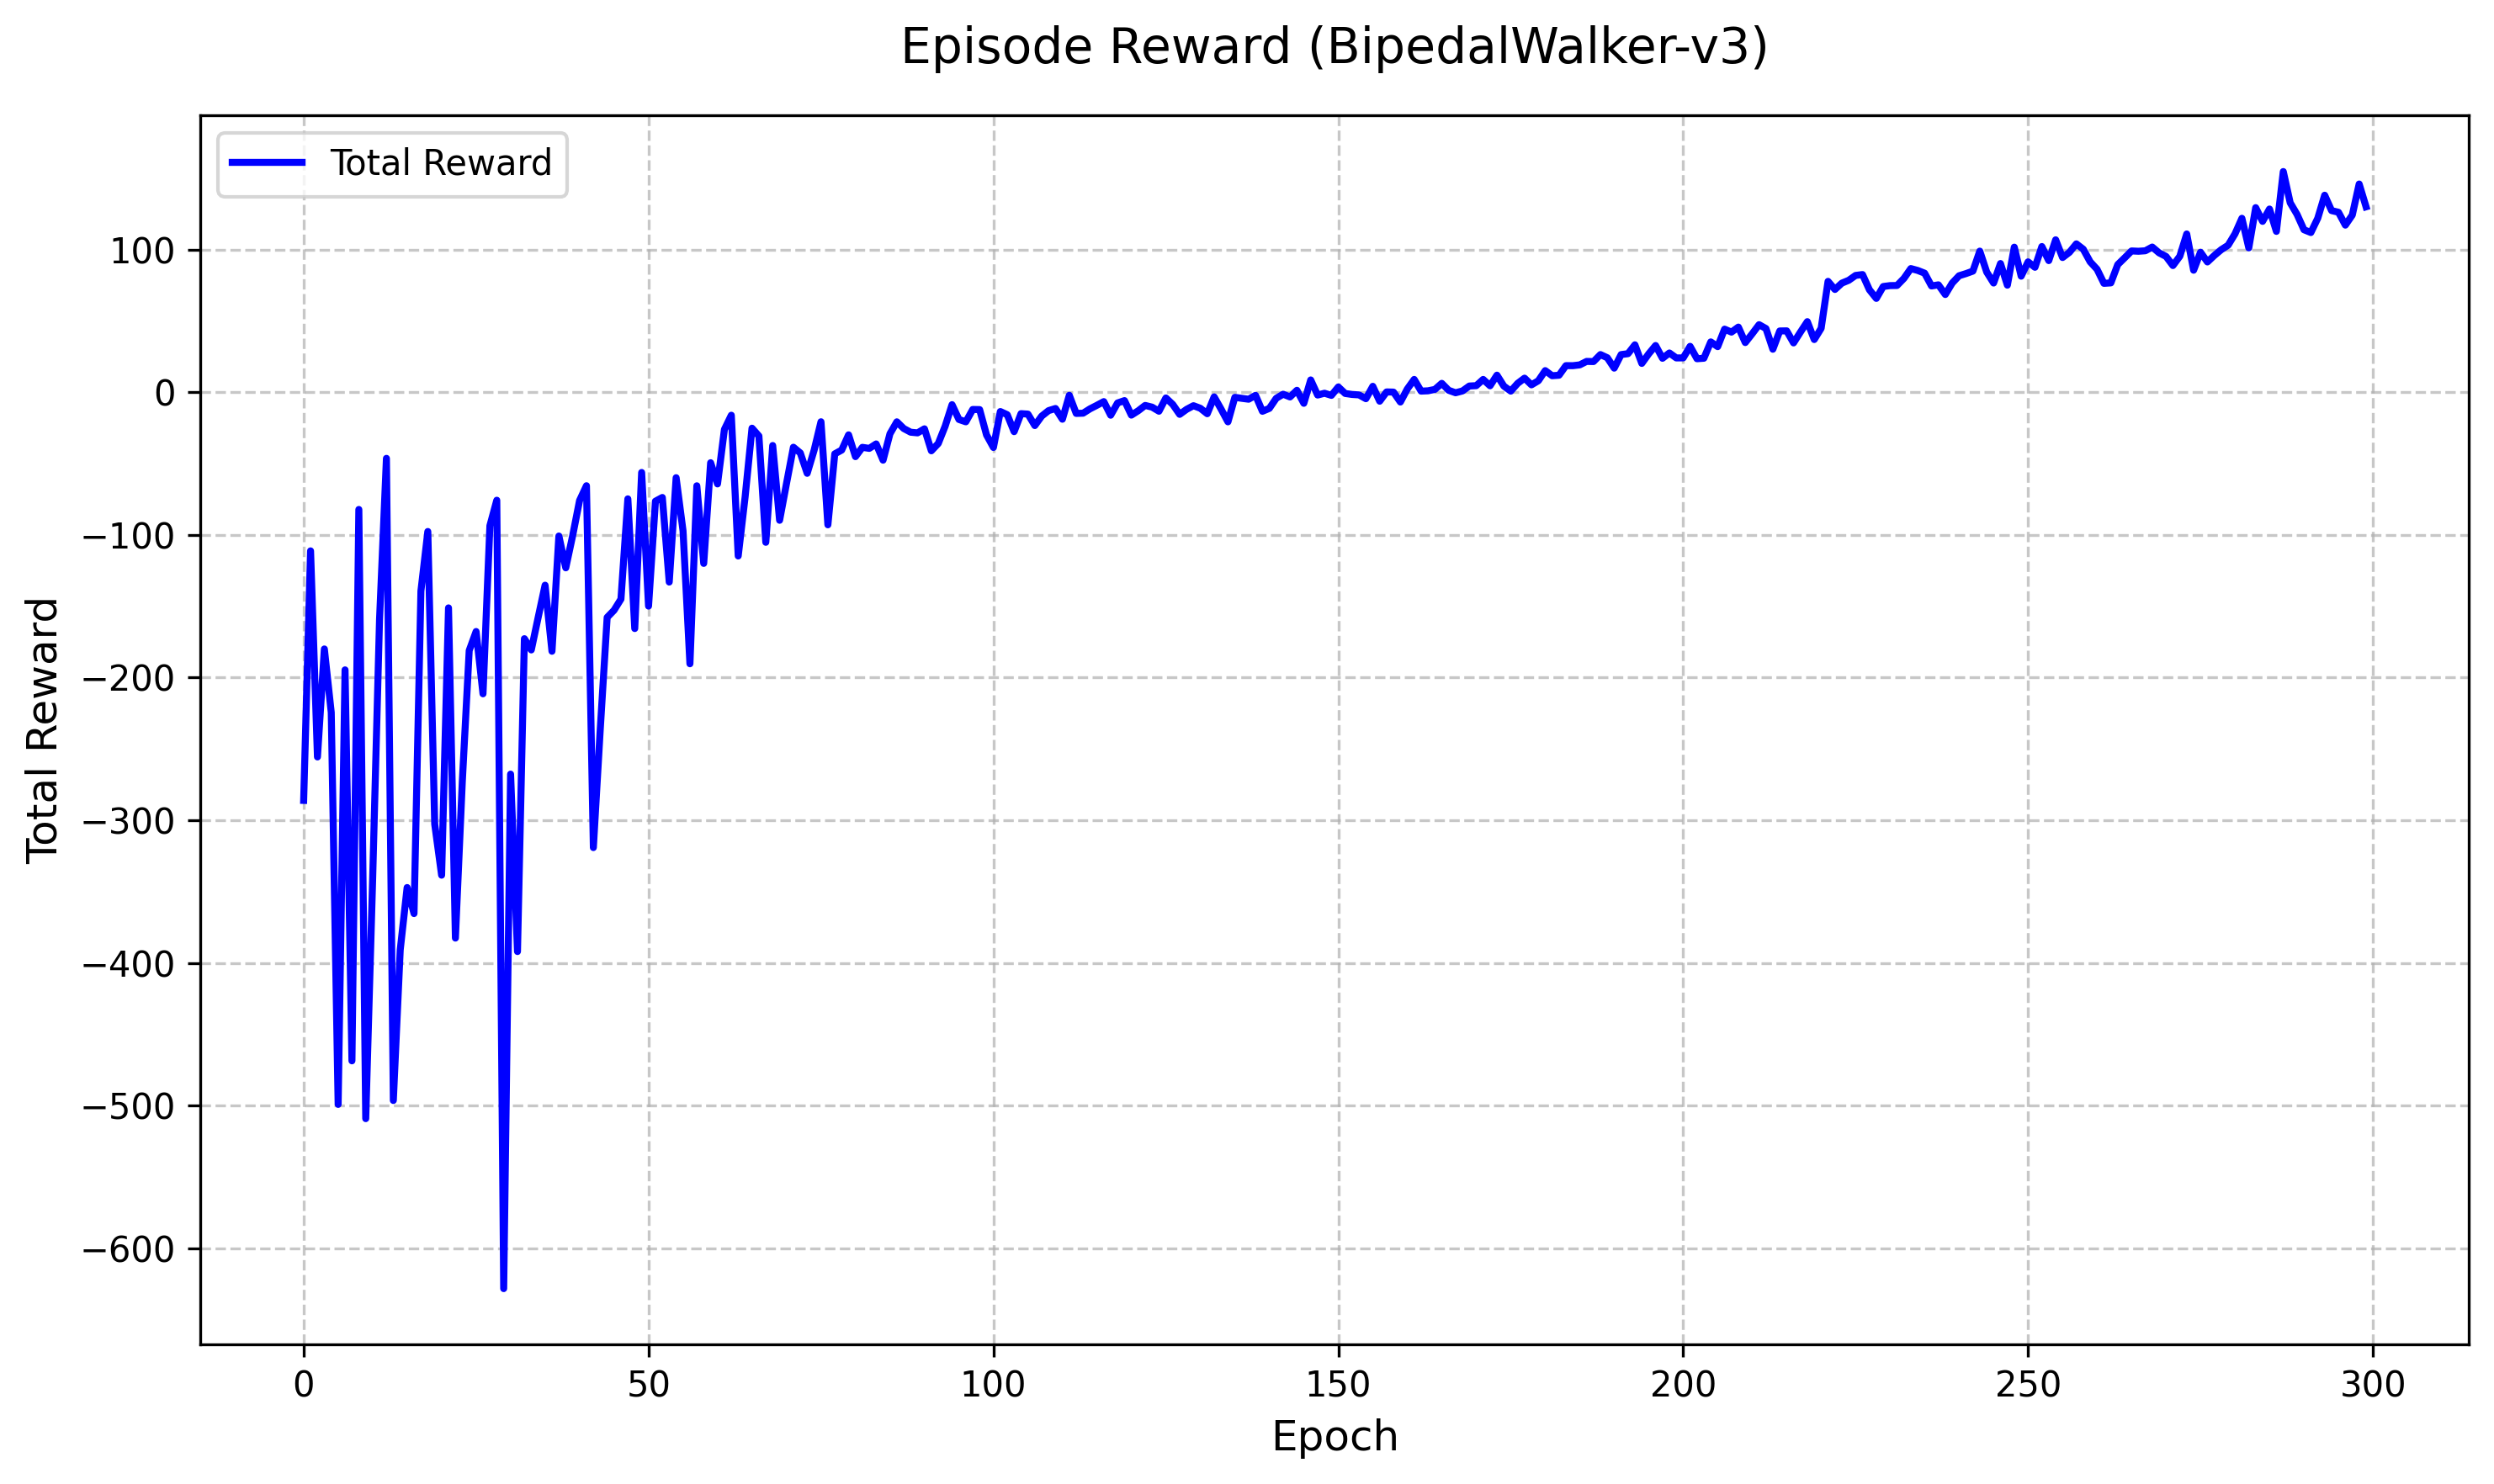
\includegraphics[width=\linewidth]{img/01-exploration--bw-03-more-exploration-large-300--reward.png}
        \caption{Reward}
    \end{subfigure}\hfill
    \begin{subfigure}{0.31\textwidth}
        \centering
        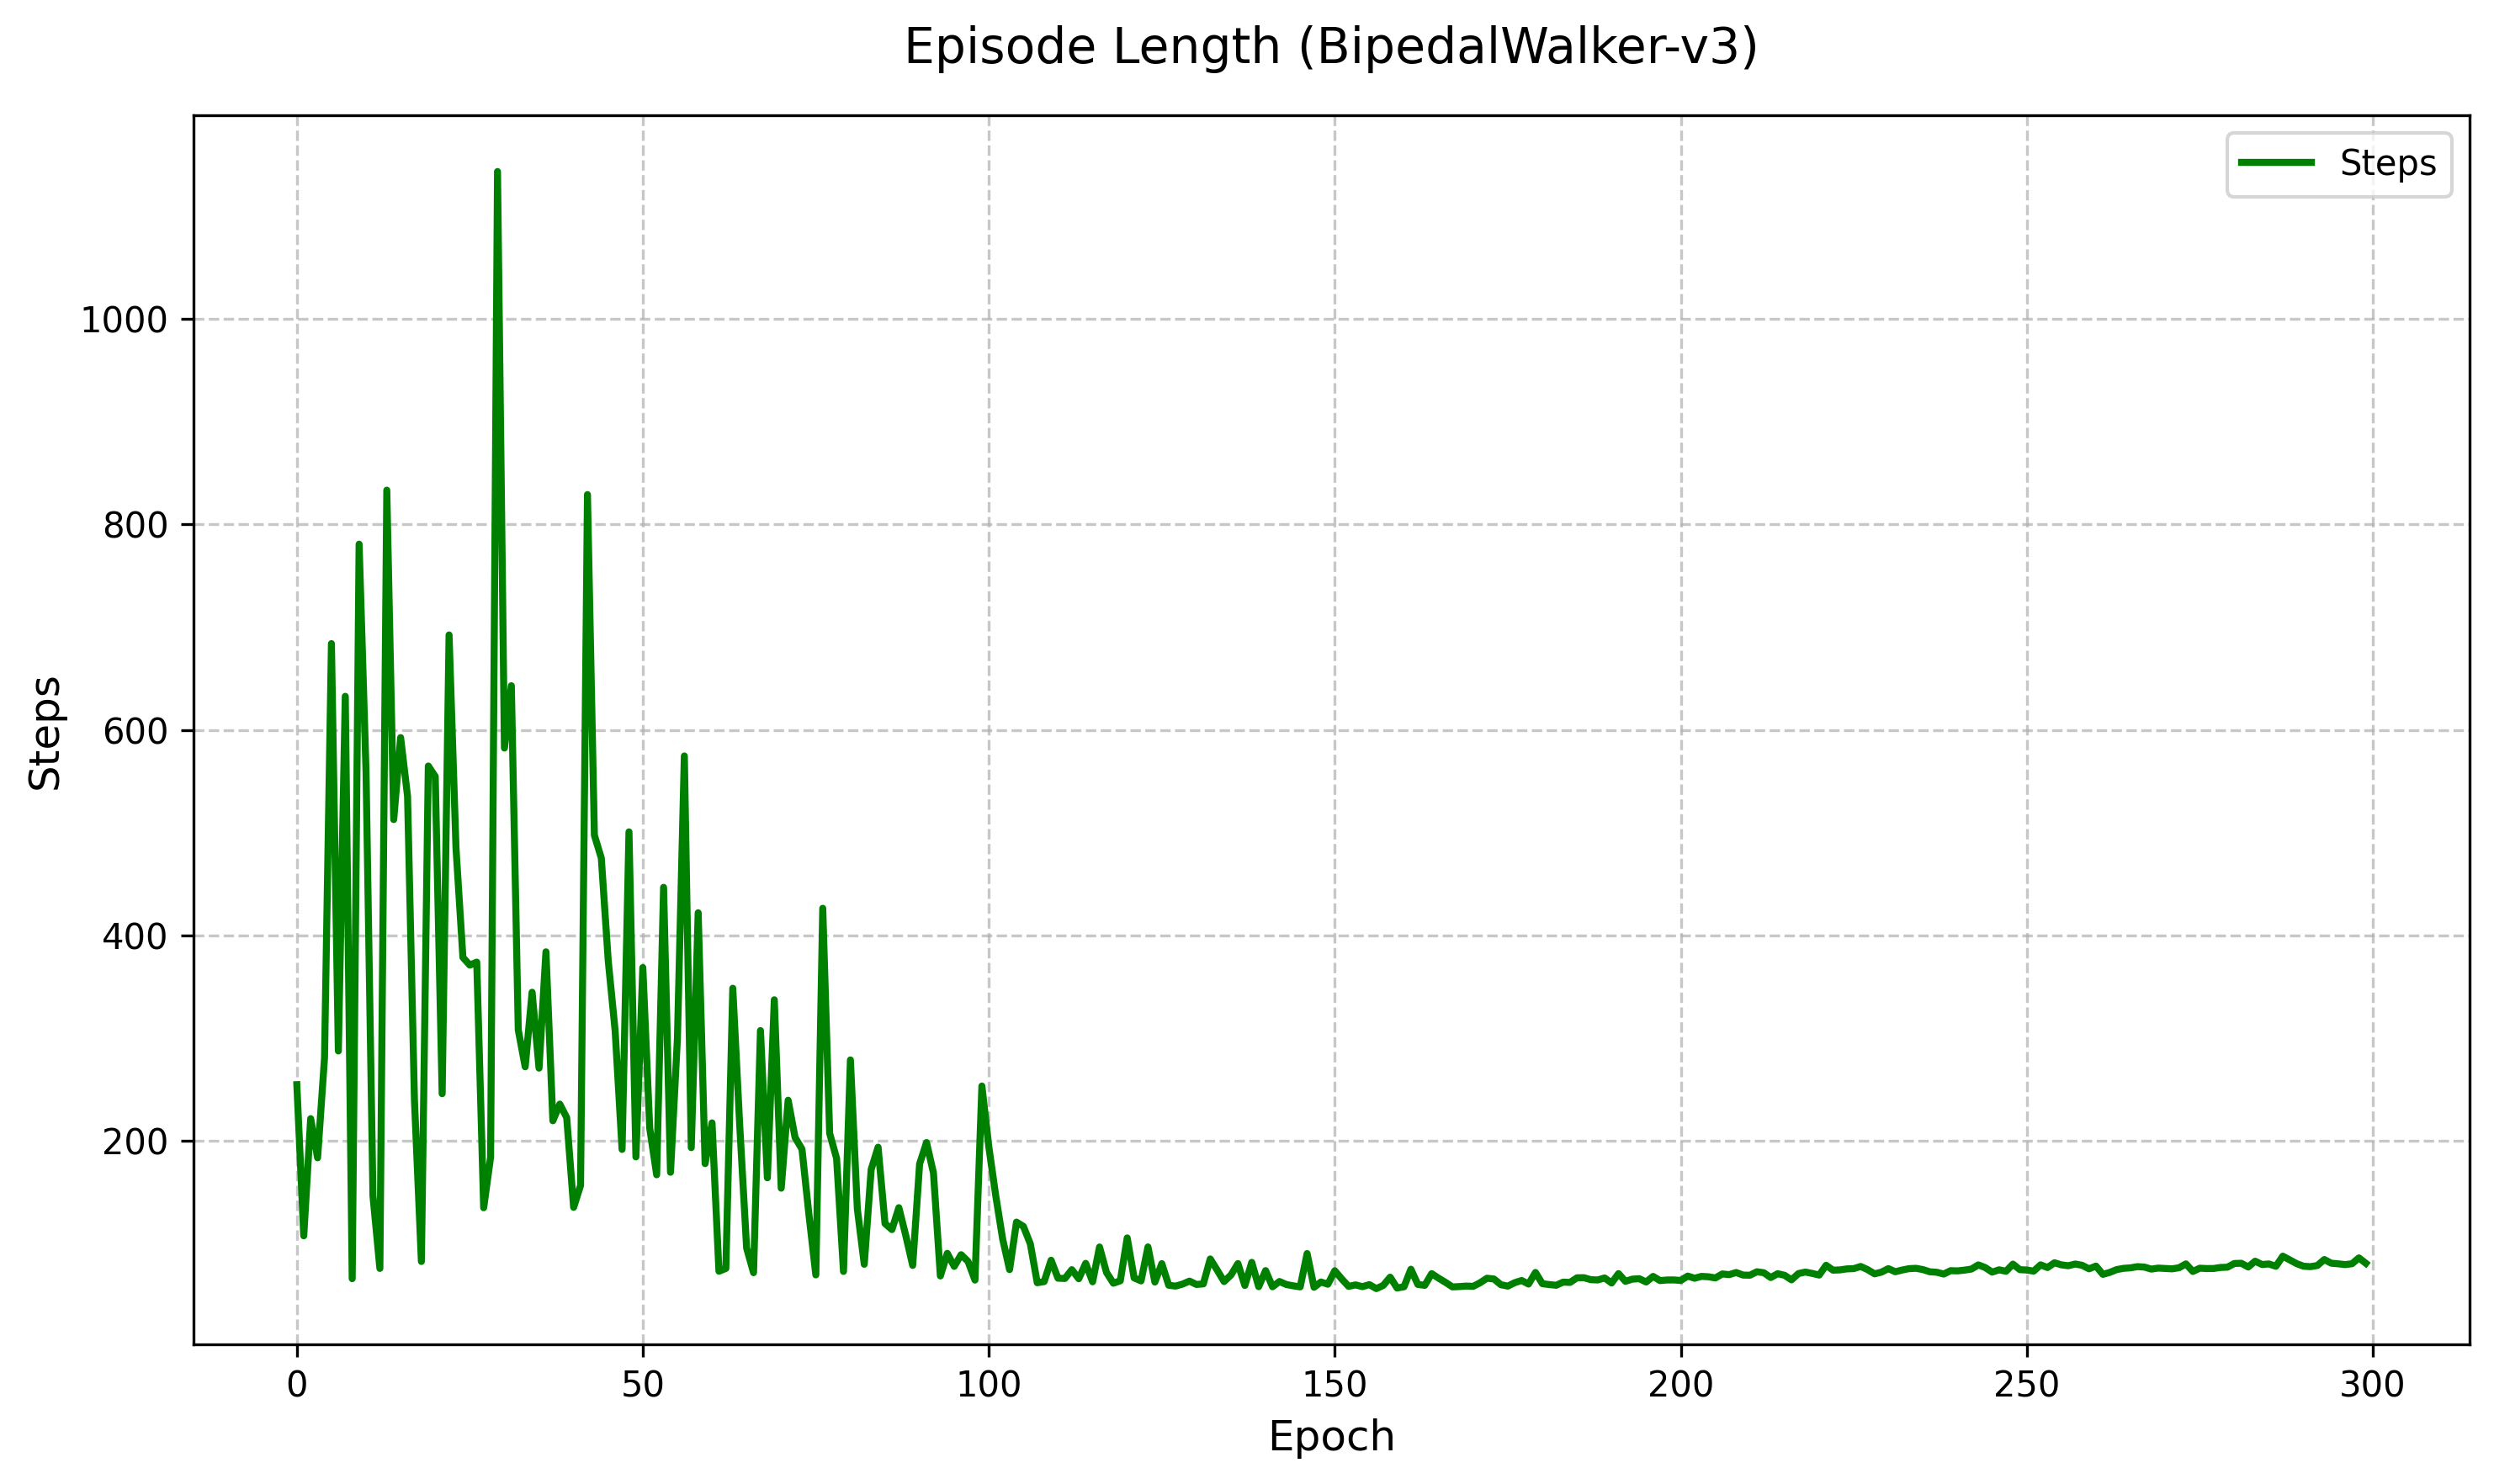
\includegraphics[width=\linewidth]{img/01-exploration--bw-03-more-exploration-large-300--length.png}
        \caption{Length}
    \end{subfigure}\hfill
    \begin{subfigure}{0.31\textwidth}
        \centering
        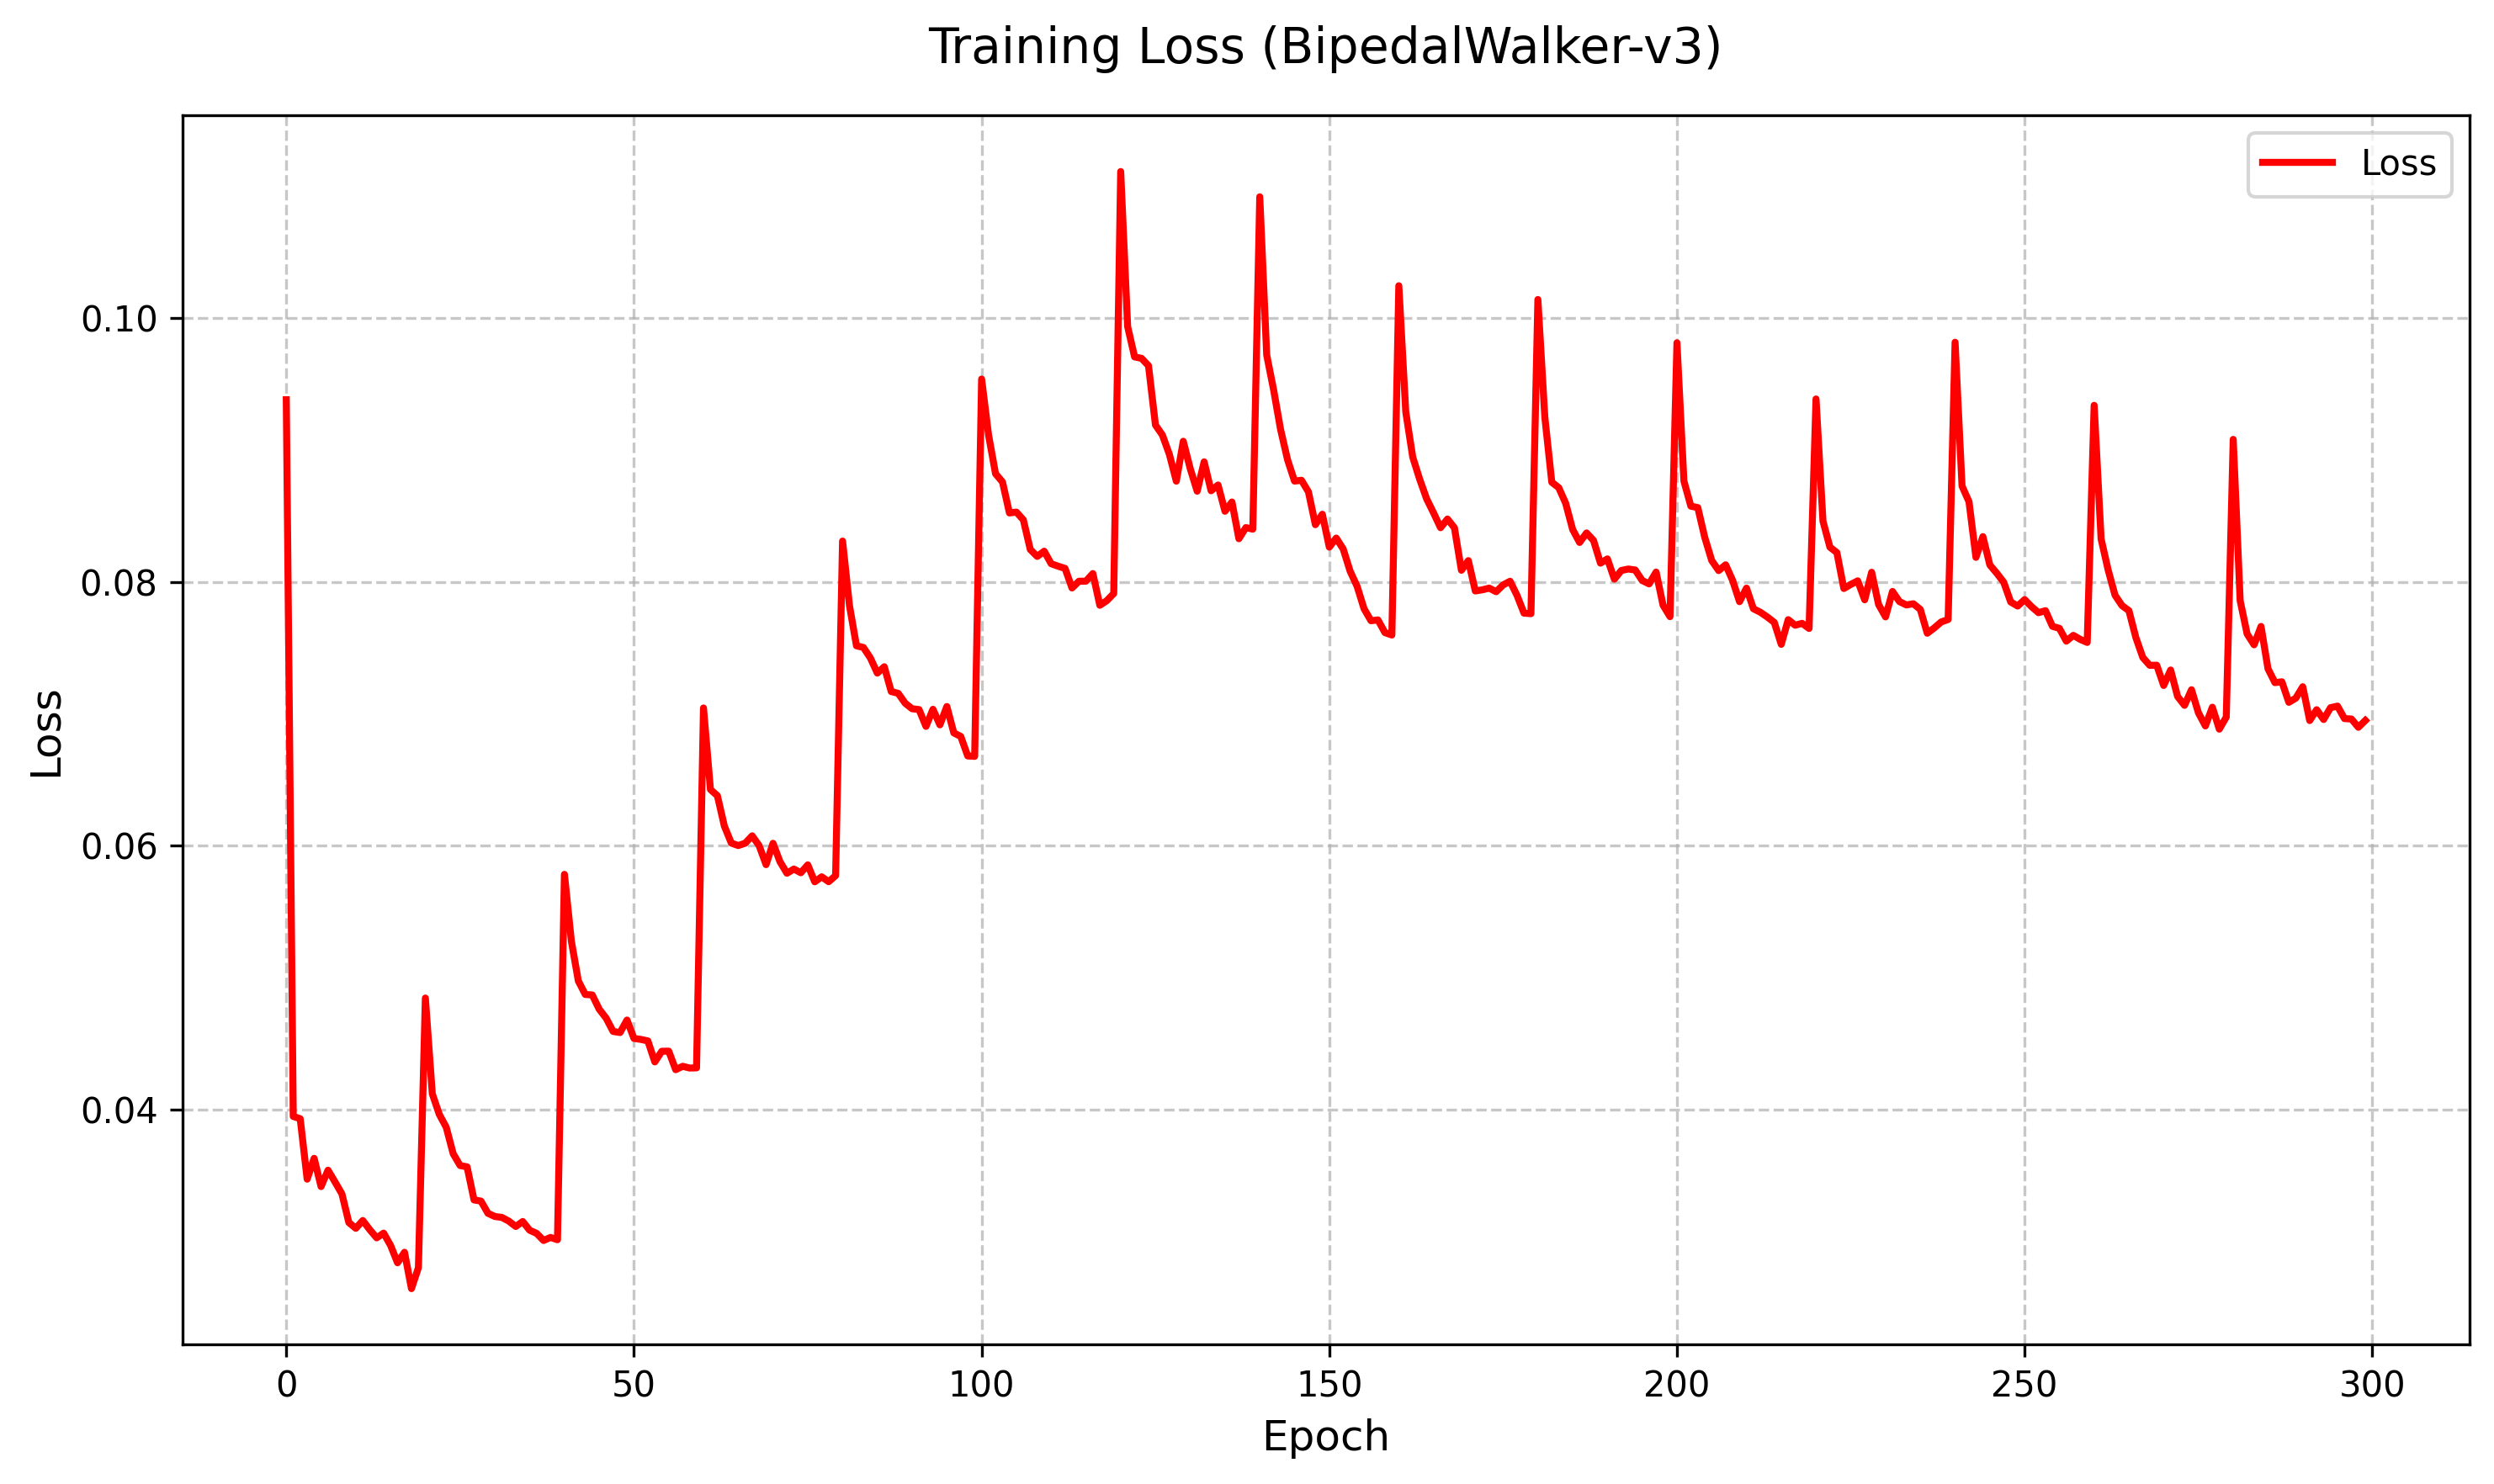
\includegraphics[width=\linewidth]{img/01-exploration--bw-03-more-exploration-large-300--loss.png}
        \caption{Loss}
    \end{subfigure}
    \caption{Category 01: Baseline vs. Increased Exploration}
    \label{fig:cat01}
\end{figure}

% 02 - Learning Rate
\begin{figure}[H]
    \centering
    \begin{subfigure}{0.31\textwidth}
        \centering
        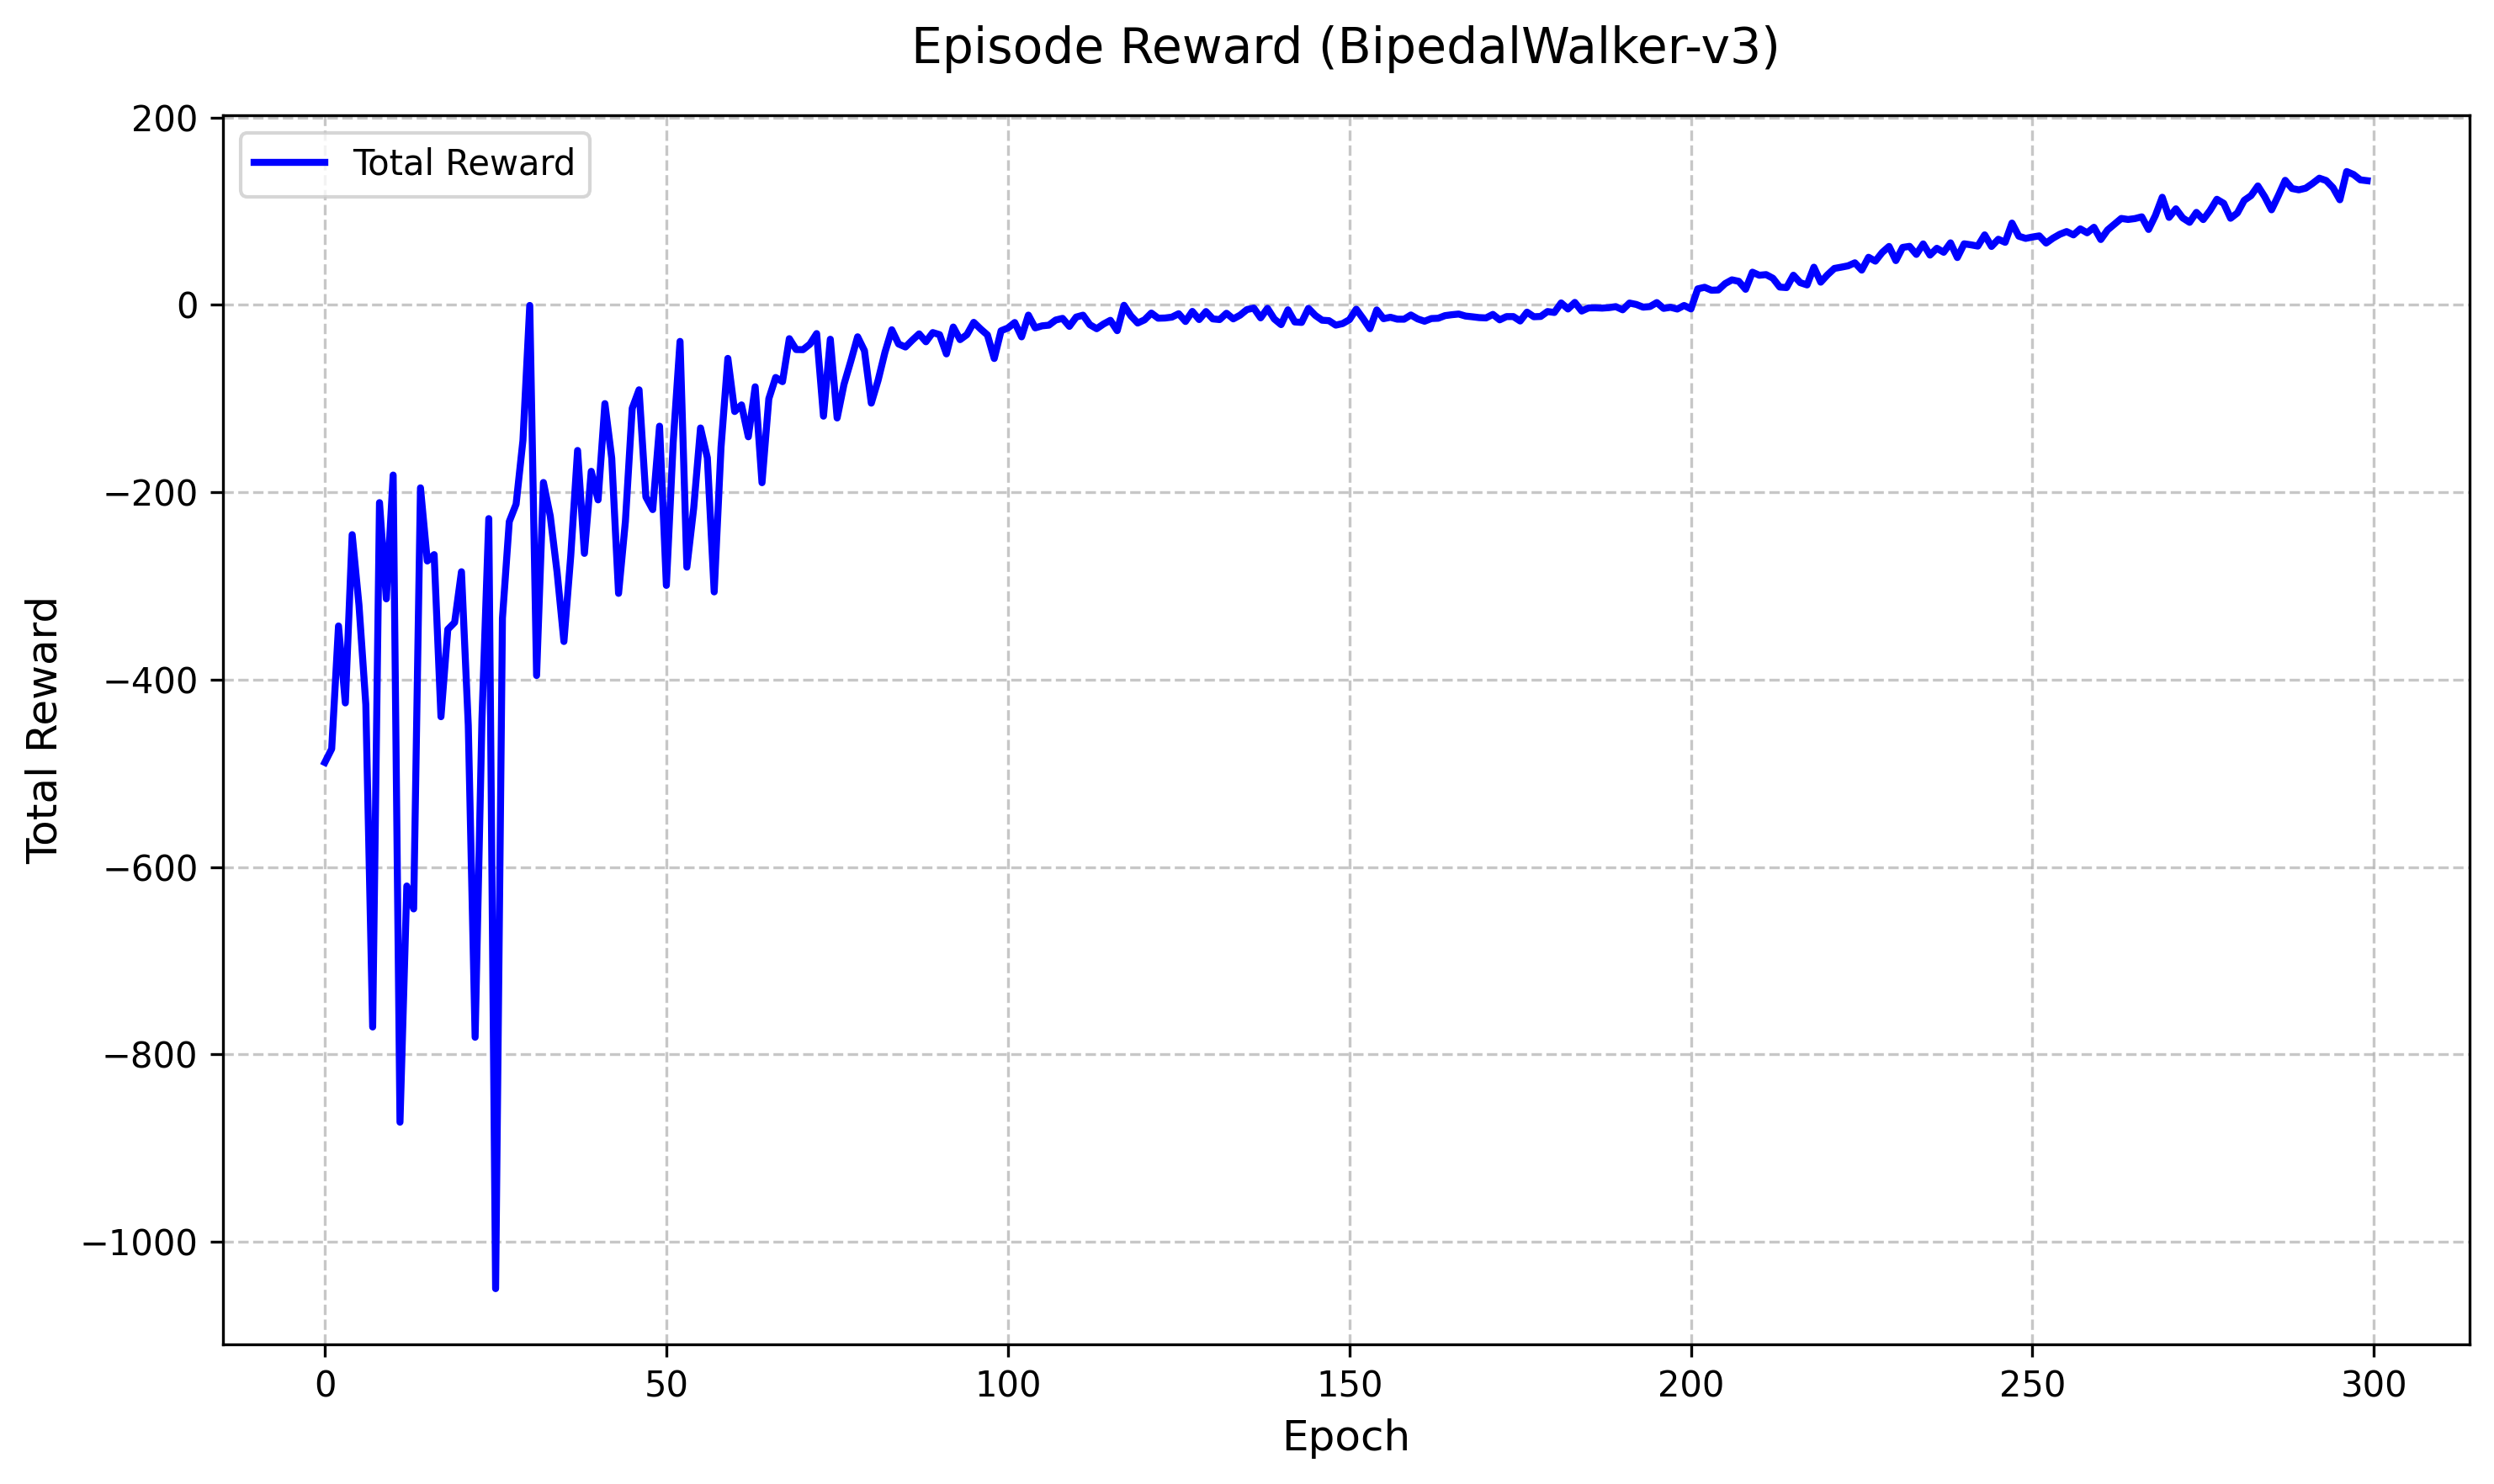
\includegraphics[width=\linewidth]{img/02-learning-rate--bw-02-stable-low-lr-large-300--reward.png}
        \caption{Reward}
    \end{subfigure}\hfill
    \begin{subfigure}{0.31\textwidth}
        \centering
        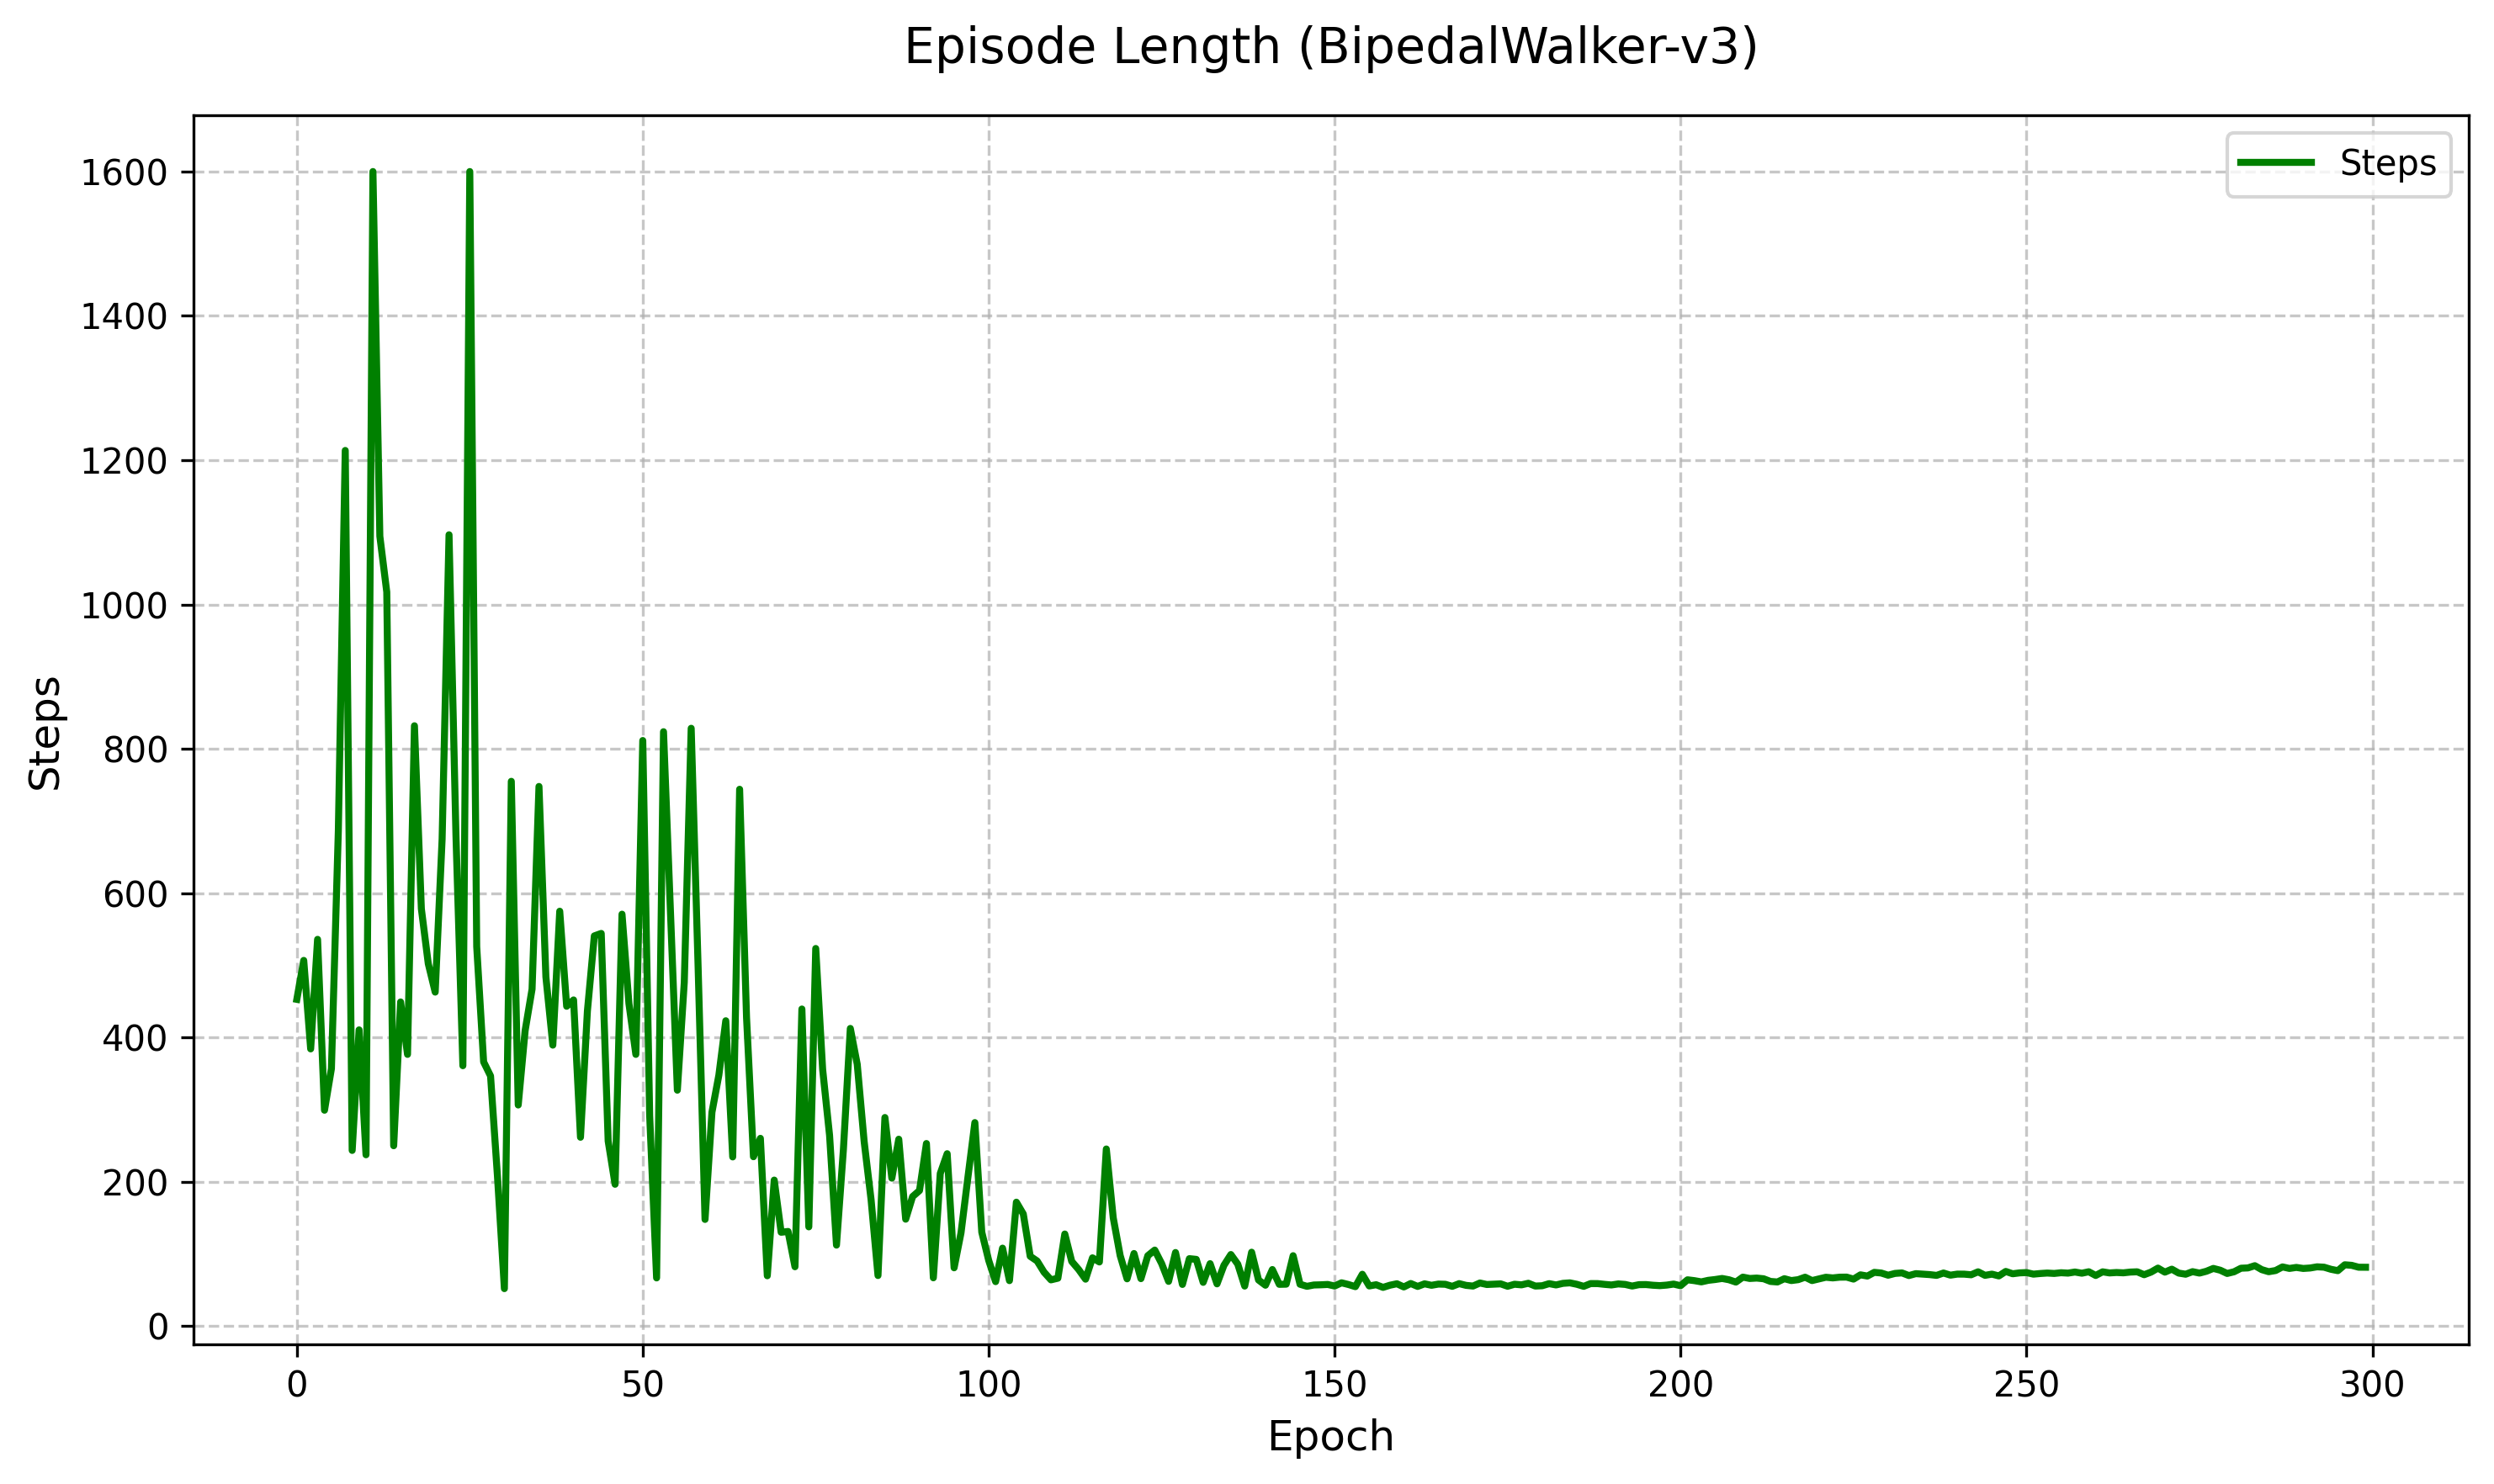
\includegraphics[width=\linewidth]{img/02-learning-rate--bw-02-stable-low-lr-large-300--length.png}
        \caption{Length}
    \end{subfigure}\hfill
    \begin{subfigure}{0.31\textwidth}
        \centering
        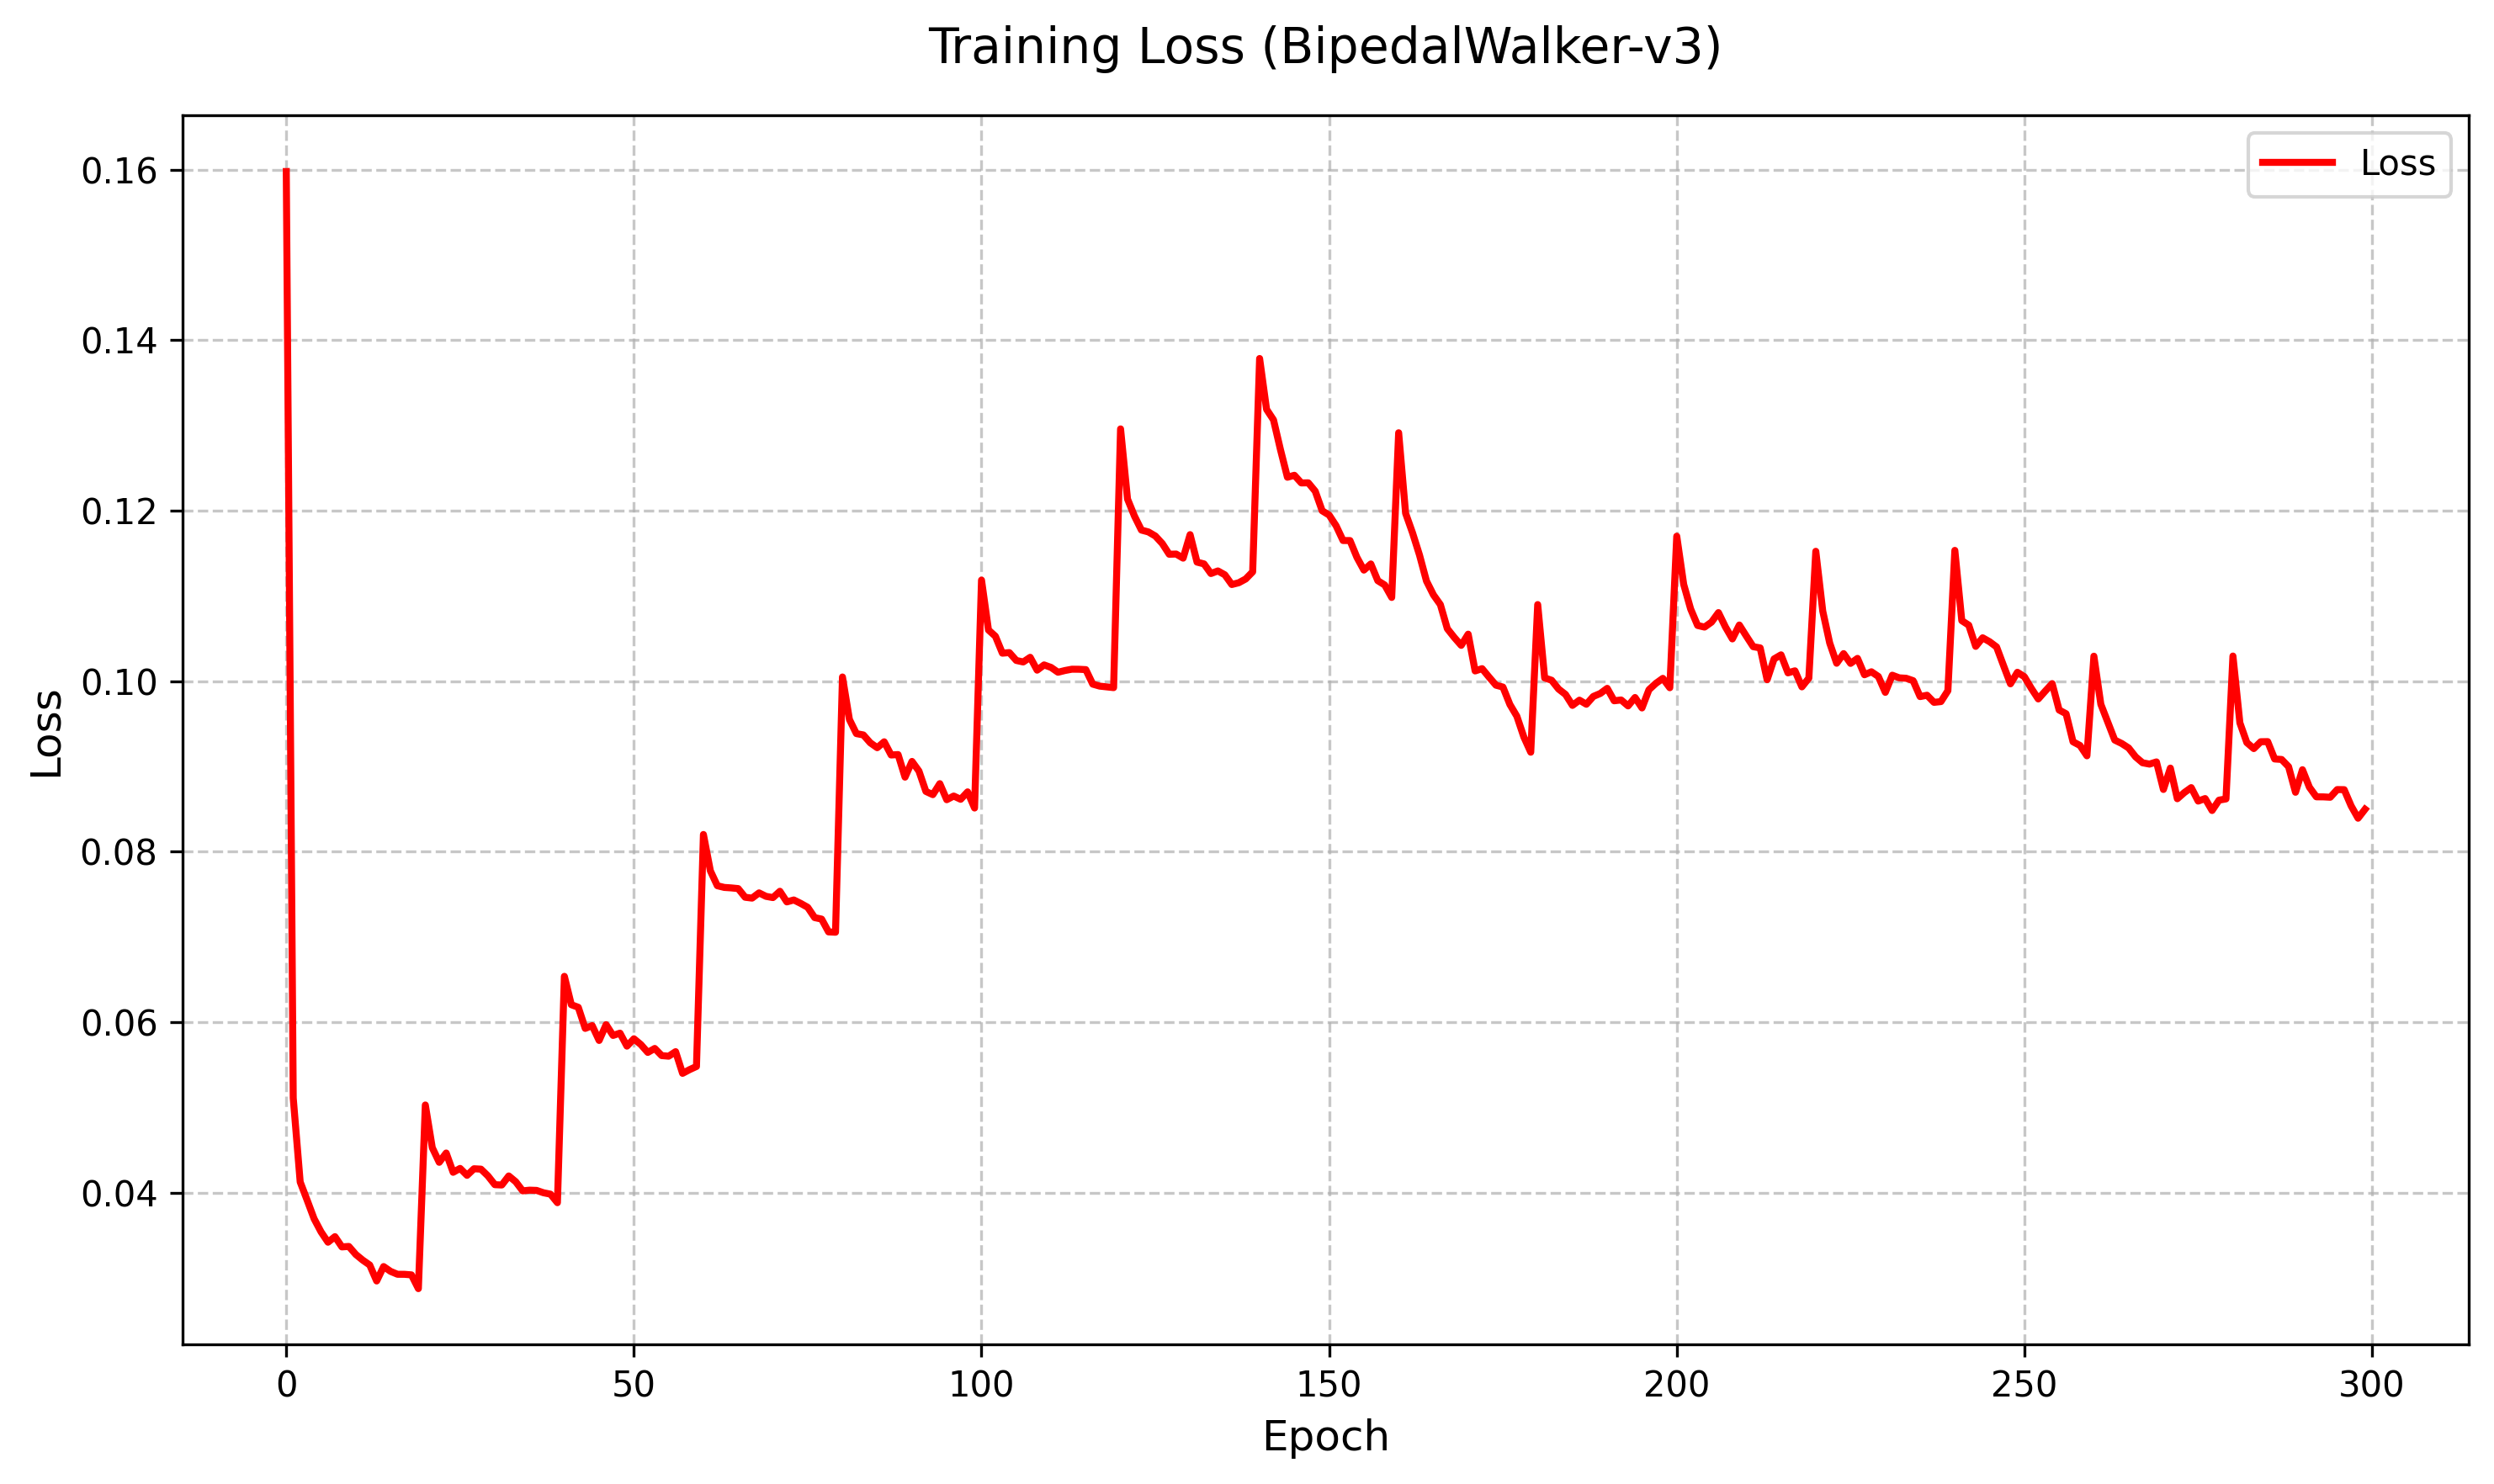
\includegraphics[width=\linewidth]{img/02-learning-rate--bw-02-stable-low-lr-large-300--loss.png}
        \caption{Loss}
    \end{subfigure}
    \caption{Category 02: Learning Rate Ablations}
\end{figure}

% 03 - Network Size
\begin{figure}[H]
    \centering
    \begin{subfigure}{0.31\textwidth}
        \centering
        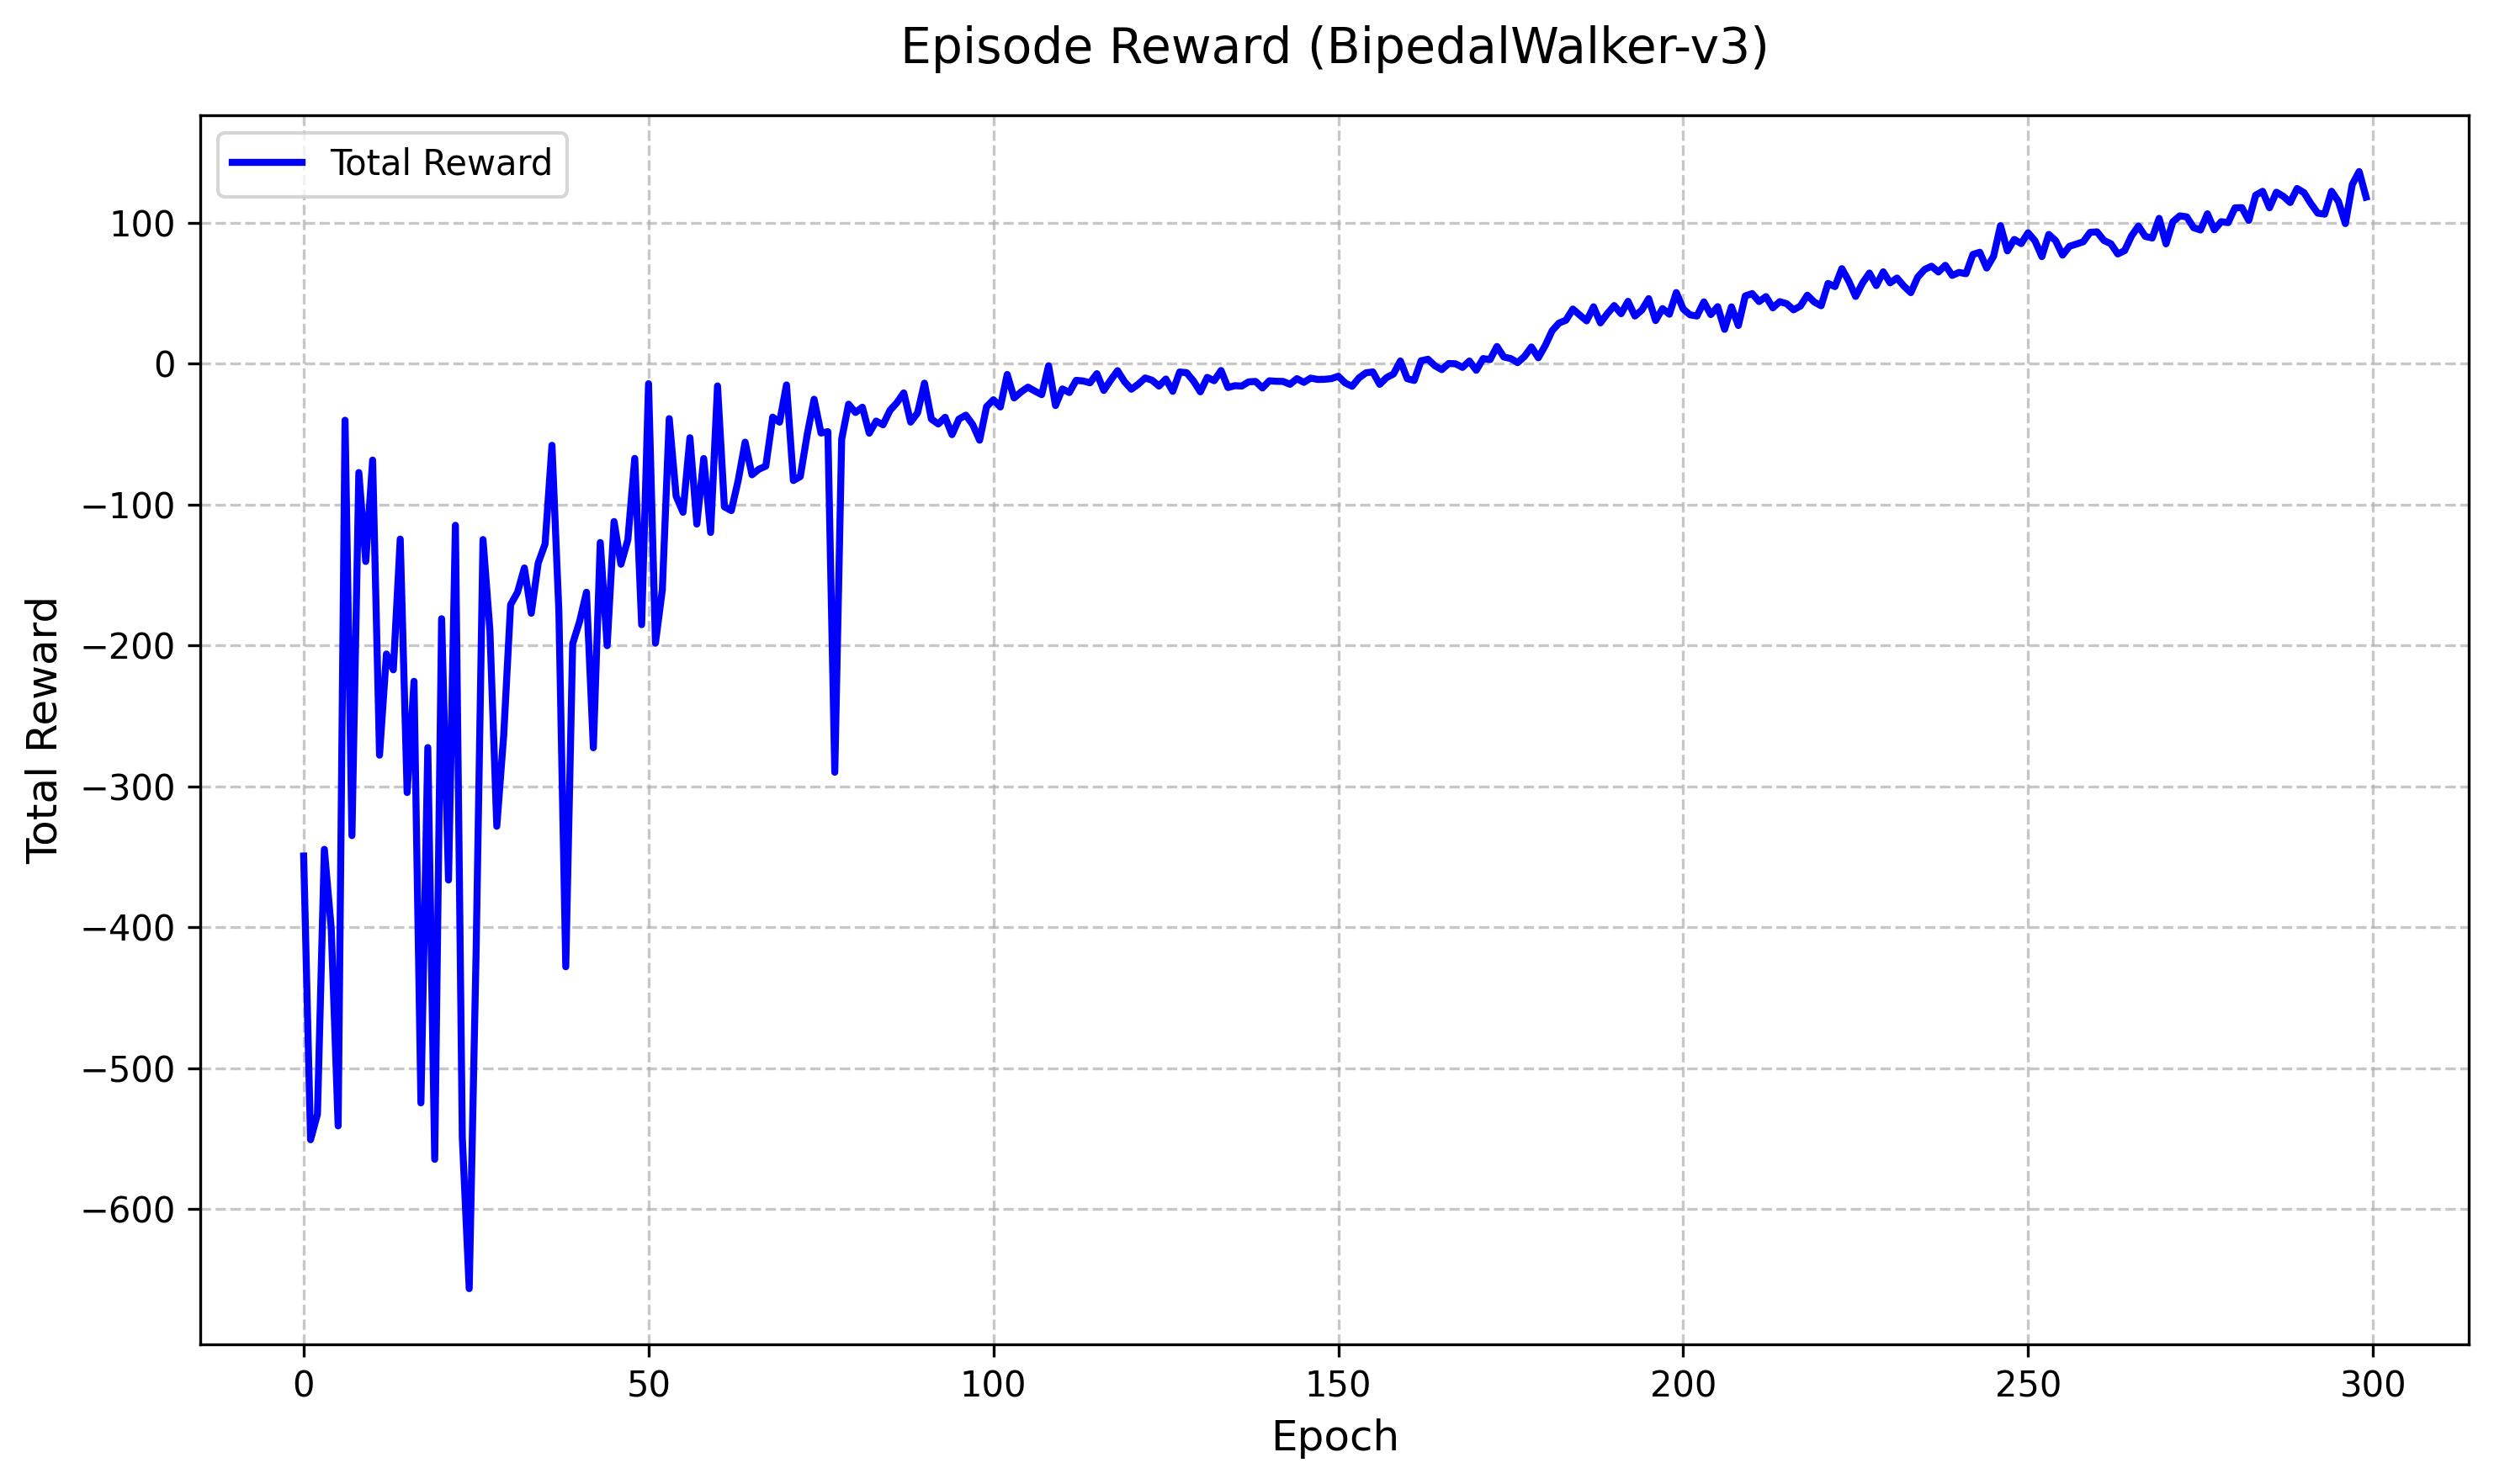
\includegraphics[width=\linewidth]{img/03-architecture--bw-04-medium-network-300--reward.png}
        \caption{Reward}
    \end{subfigure}\hfill
    \begin{subfigure}{0.31\textwidth}
        \centering
        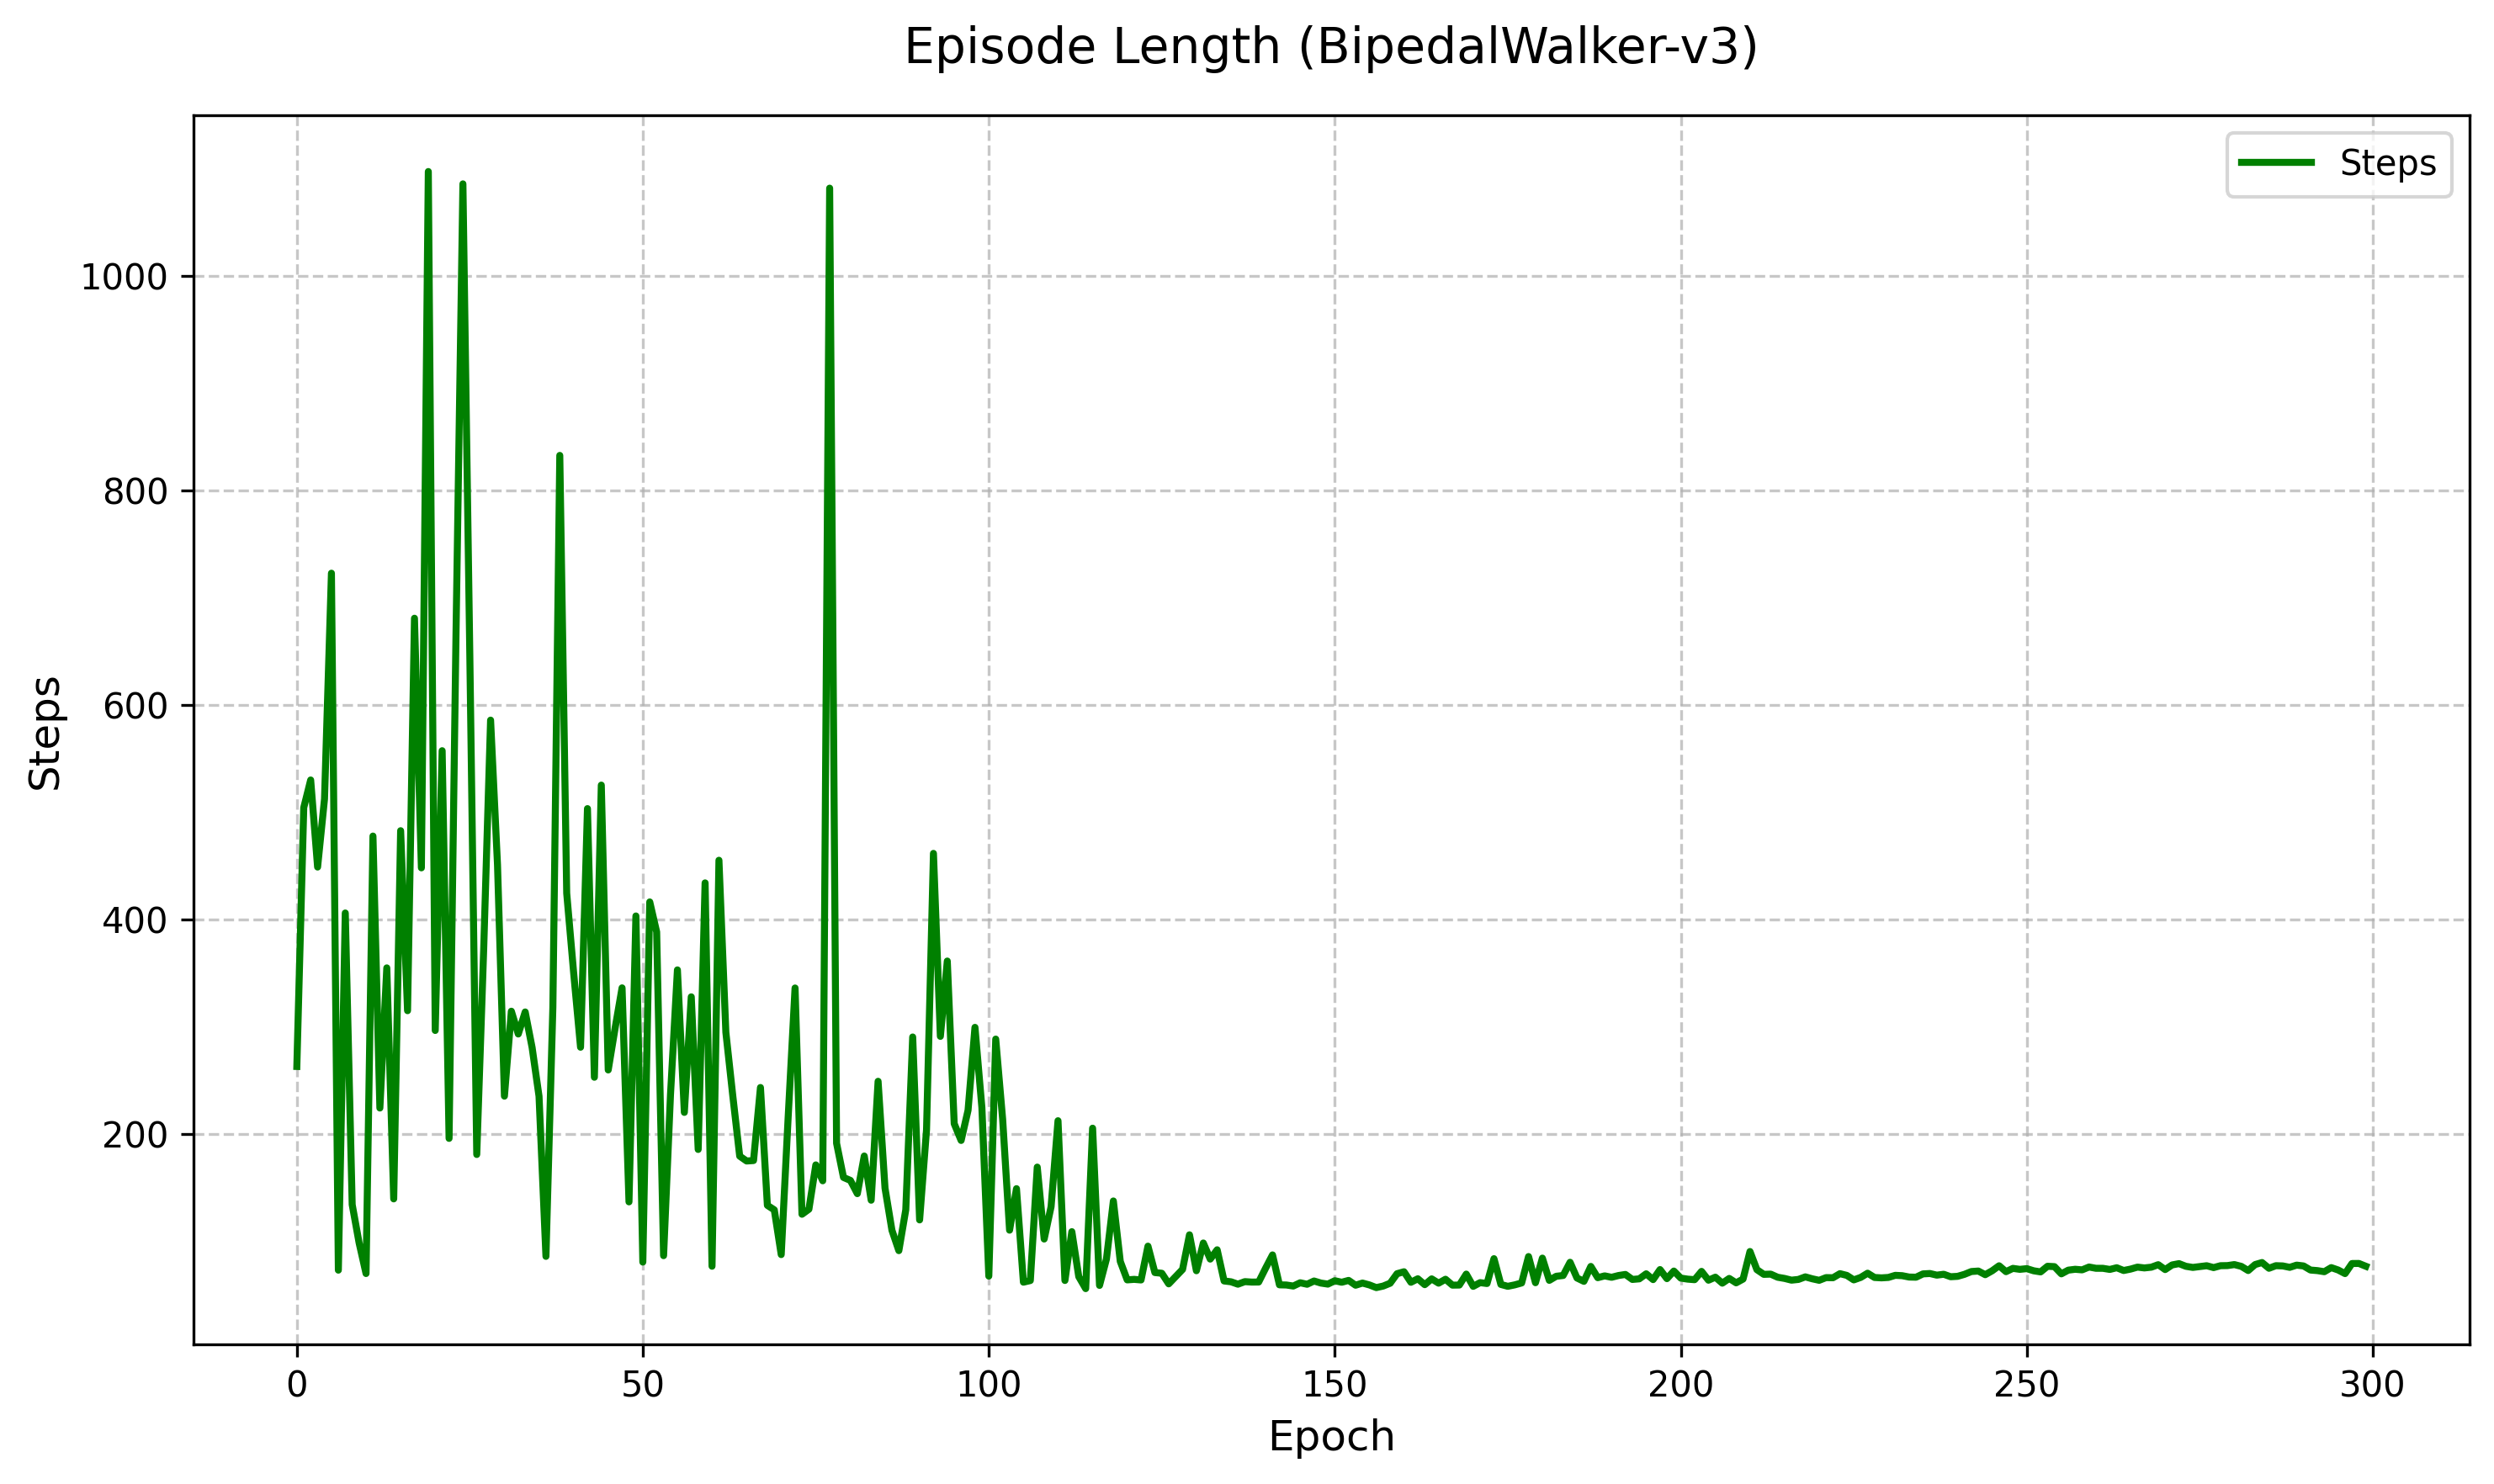
\includegraphics[width=\linewidth]{img/03-architecture--bw-04-medium-network-300--length.png}
        \caption{Length}
    \end{subfigure}\hfill
    \begin{subfigure}{0.31\textwidth}
        \centering
        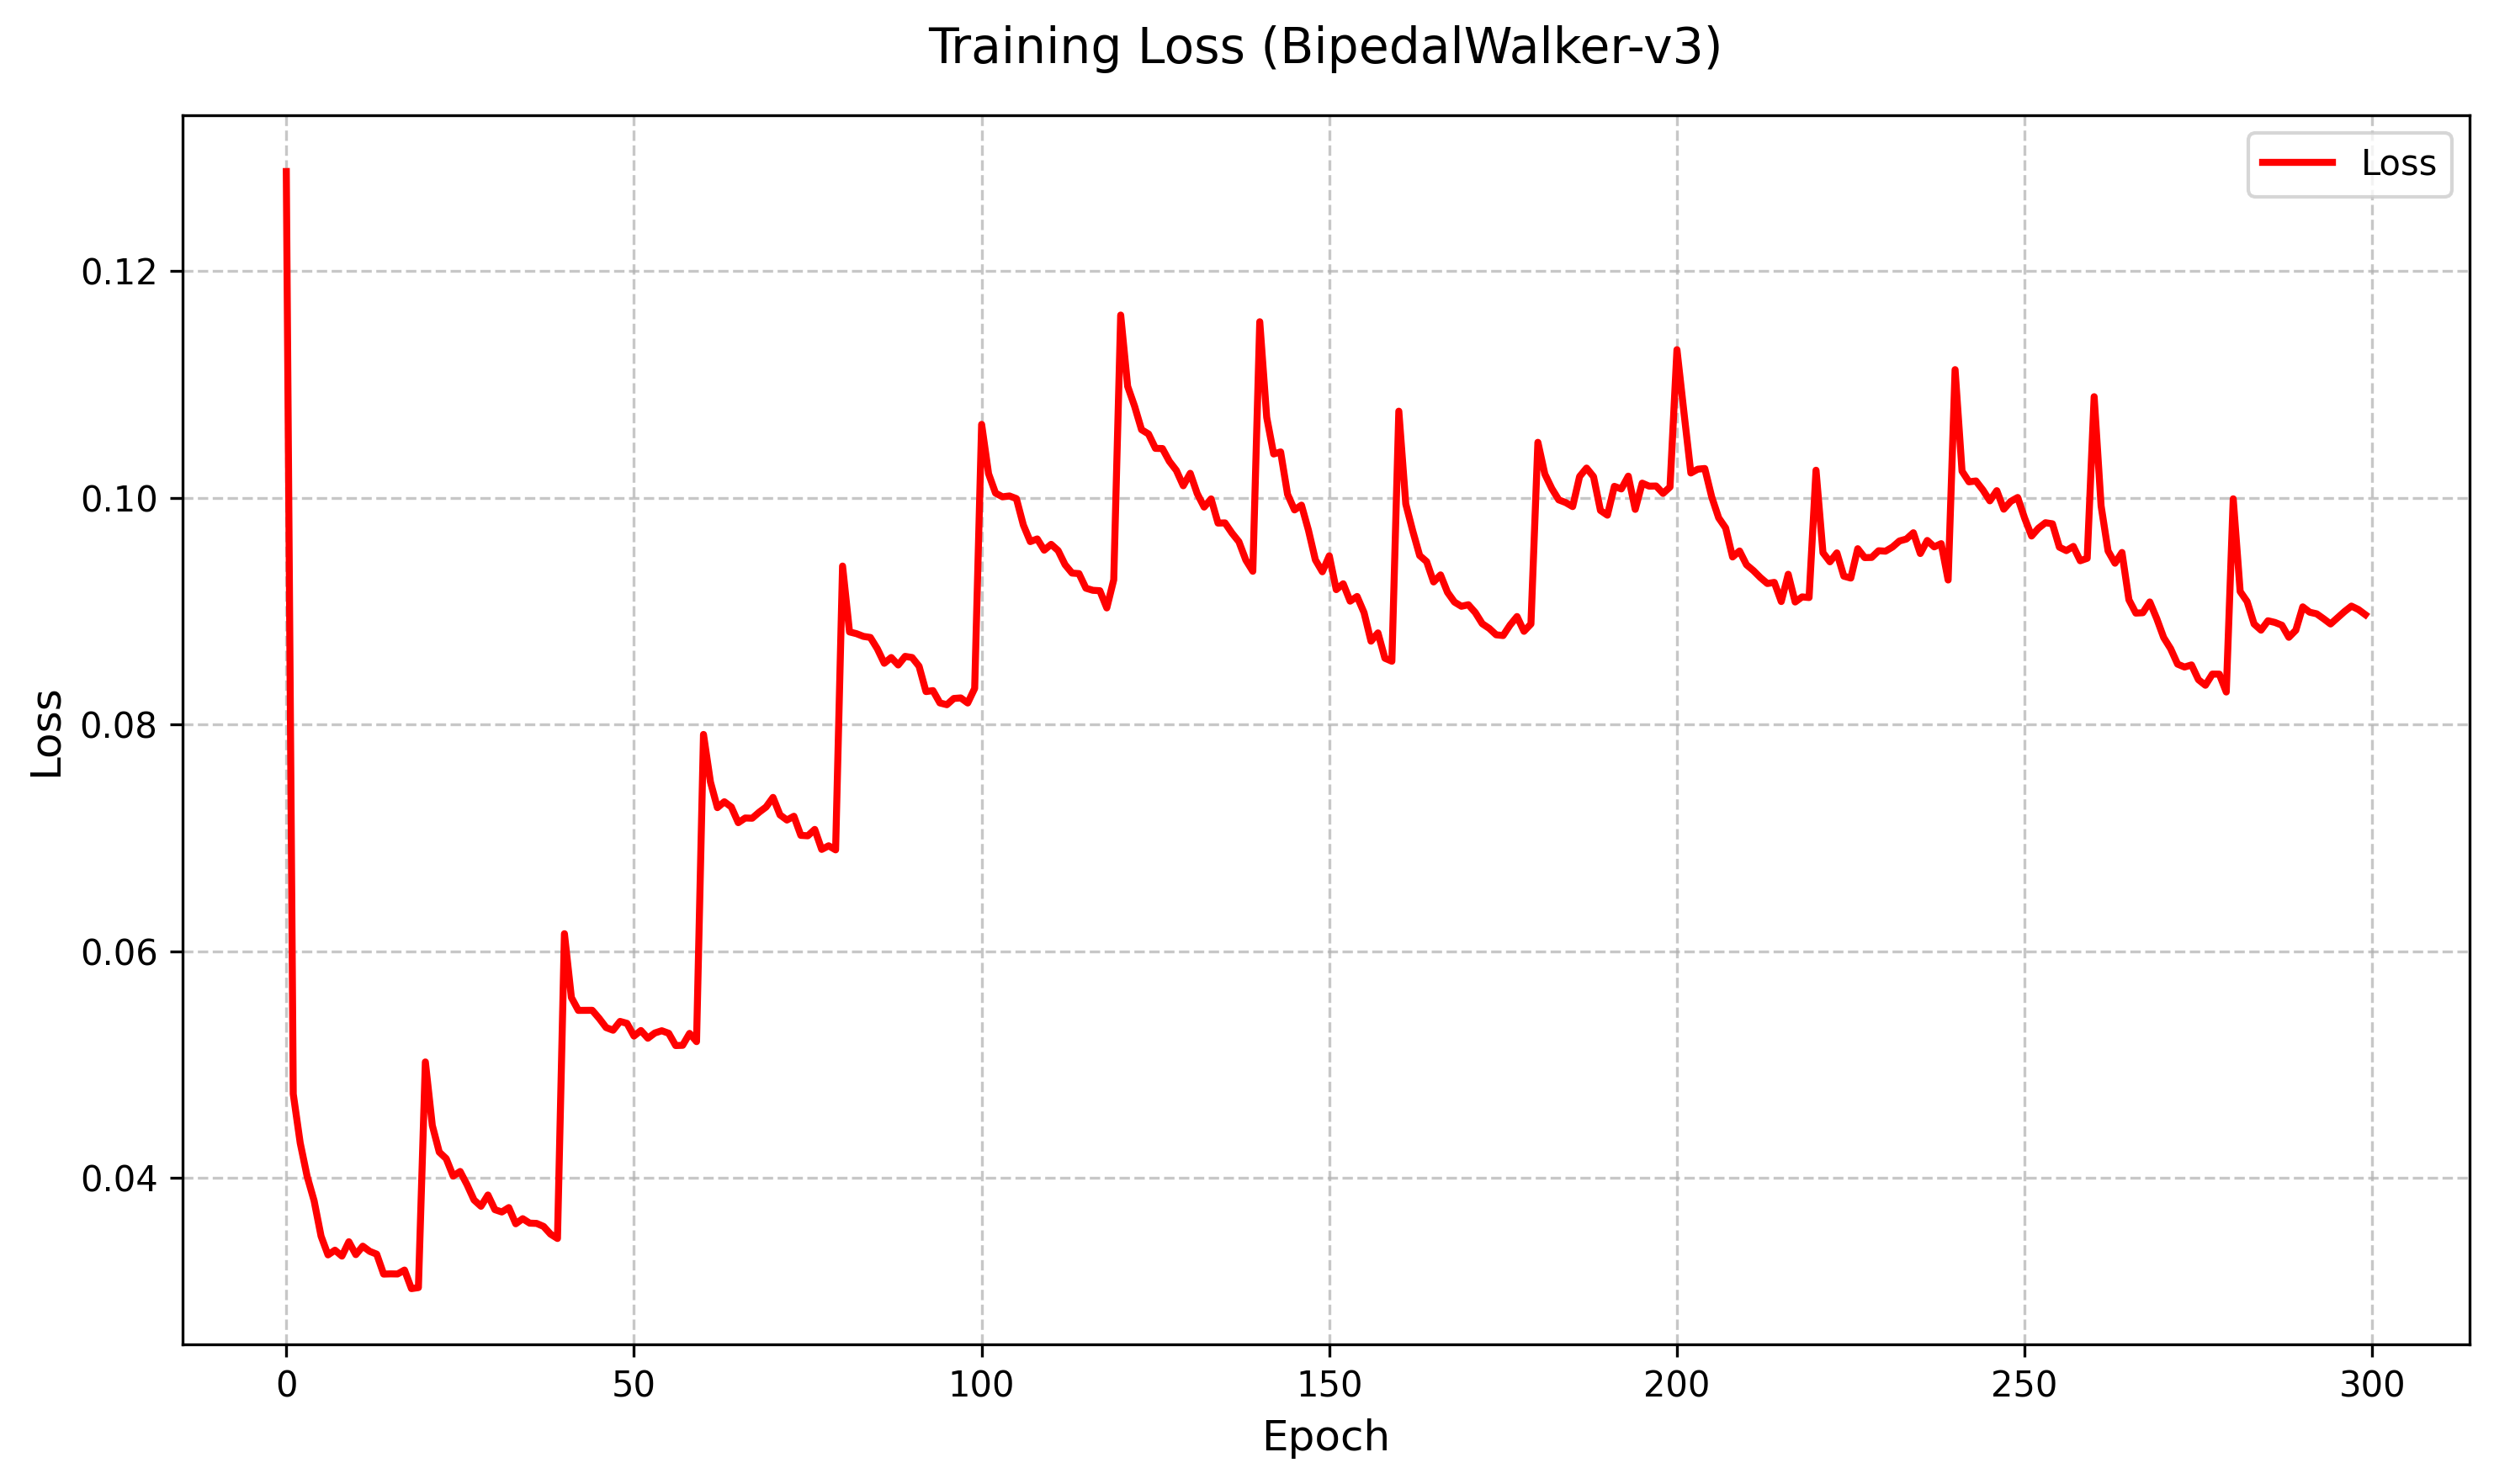
\includegraphics[width=\linewidth]{img/03-architecture--bw-04-medium-network-300--loss.png}
        \caption{Loss}
    \end{subfigure}
    \caption{Category 03: Architecture Size Comparison}
\end{figure}

% 04 - Replay/Batch
\begin{figure}[H]
    \centering
    \begin{subfigure}{0.31\textwidth}
        \centering
        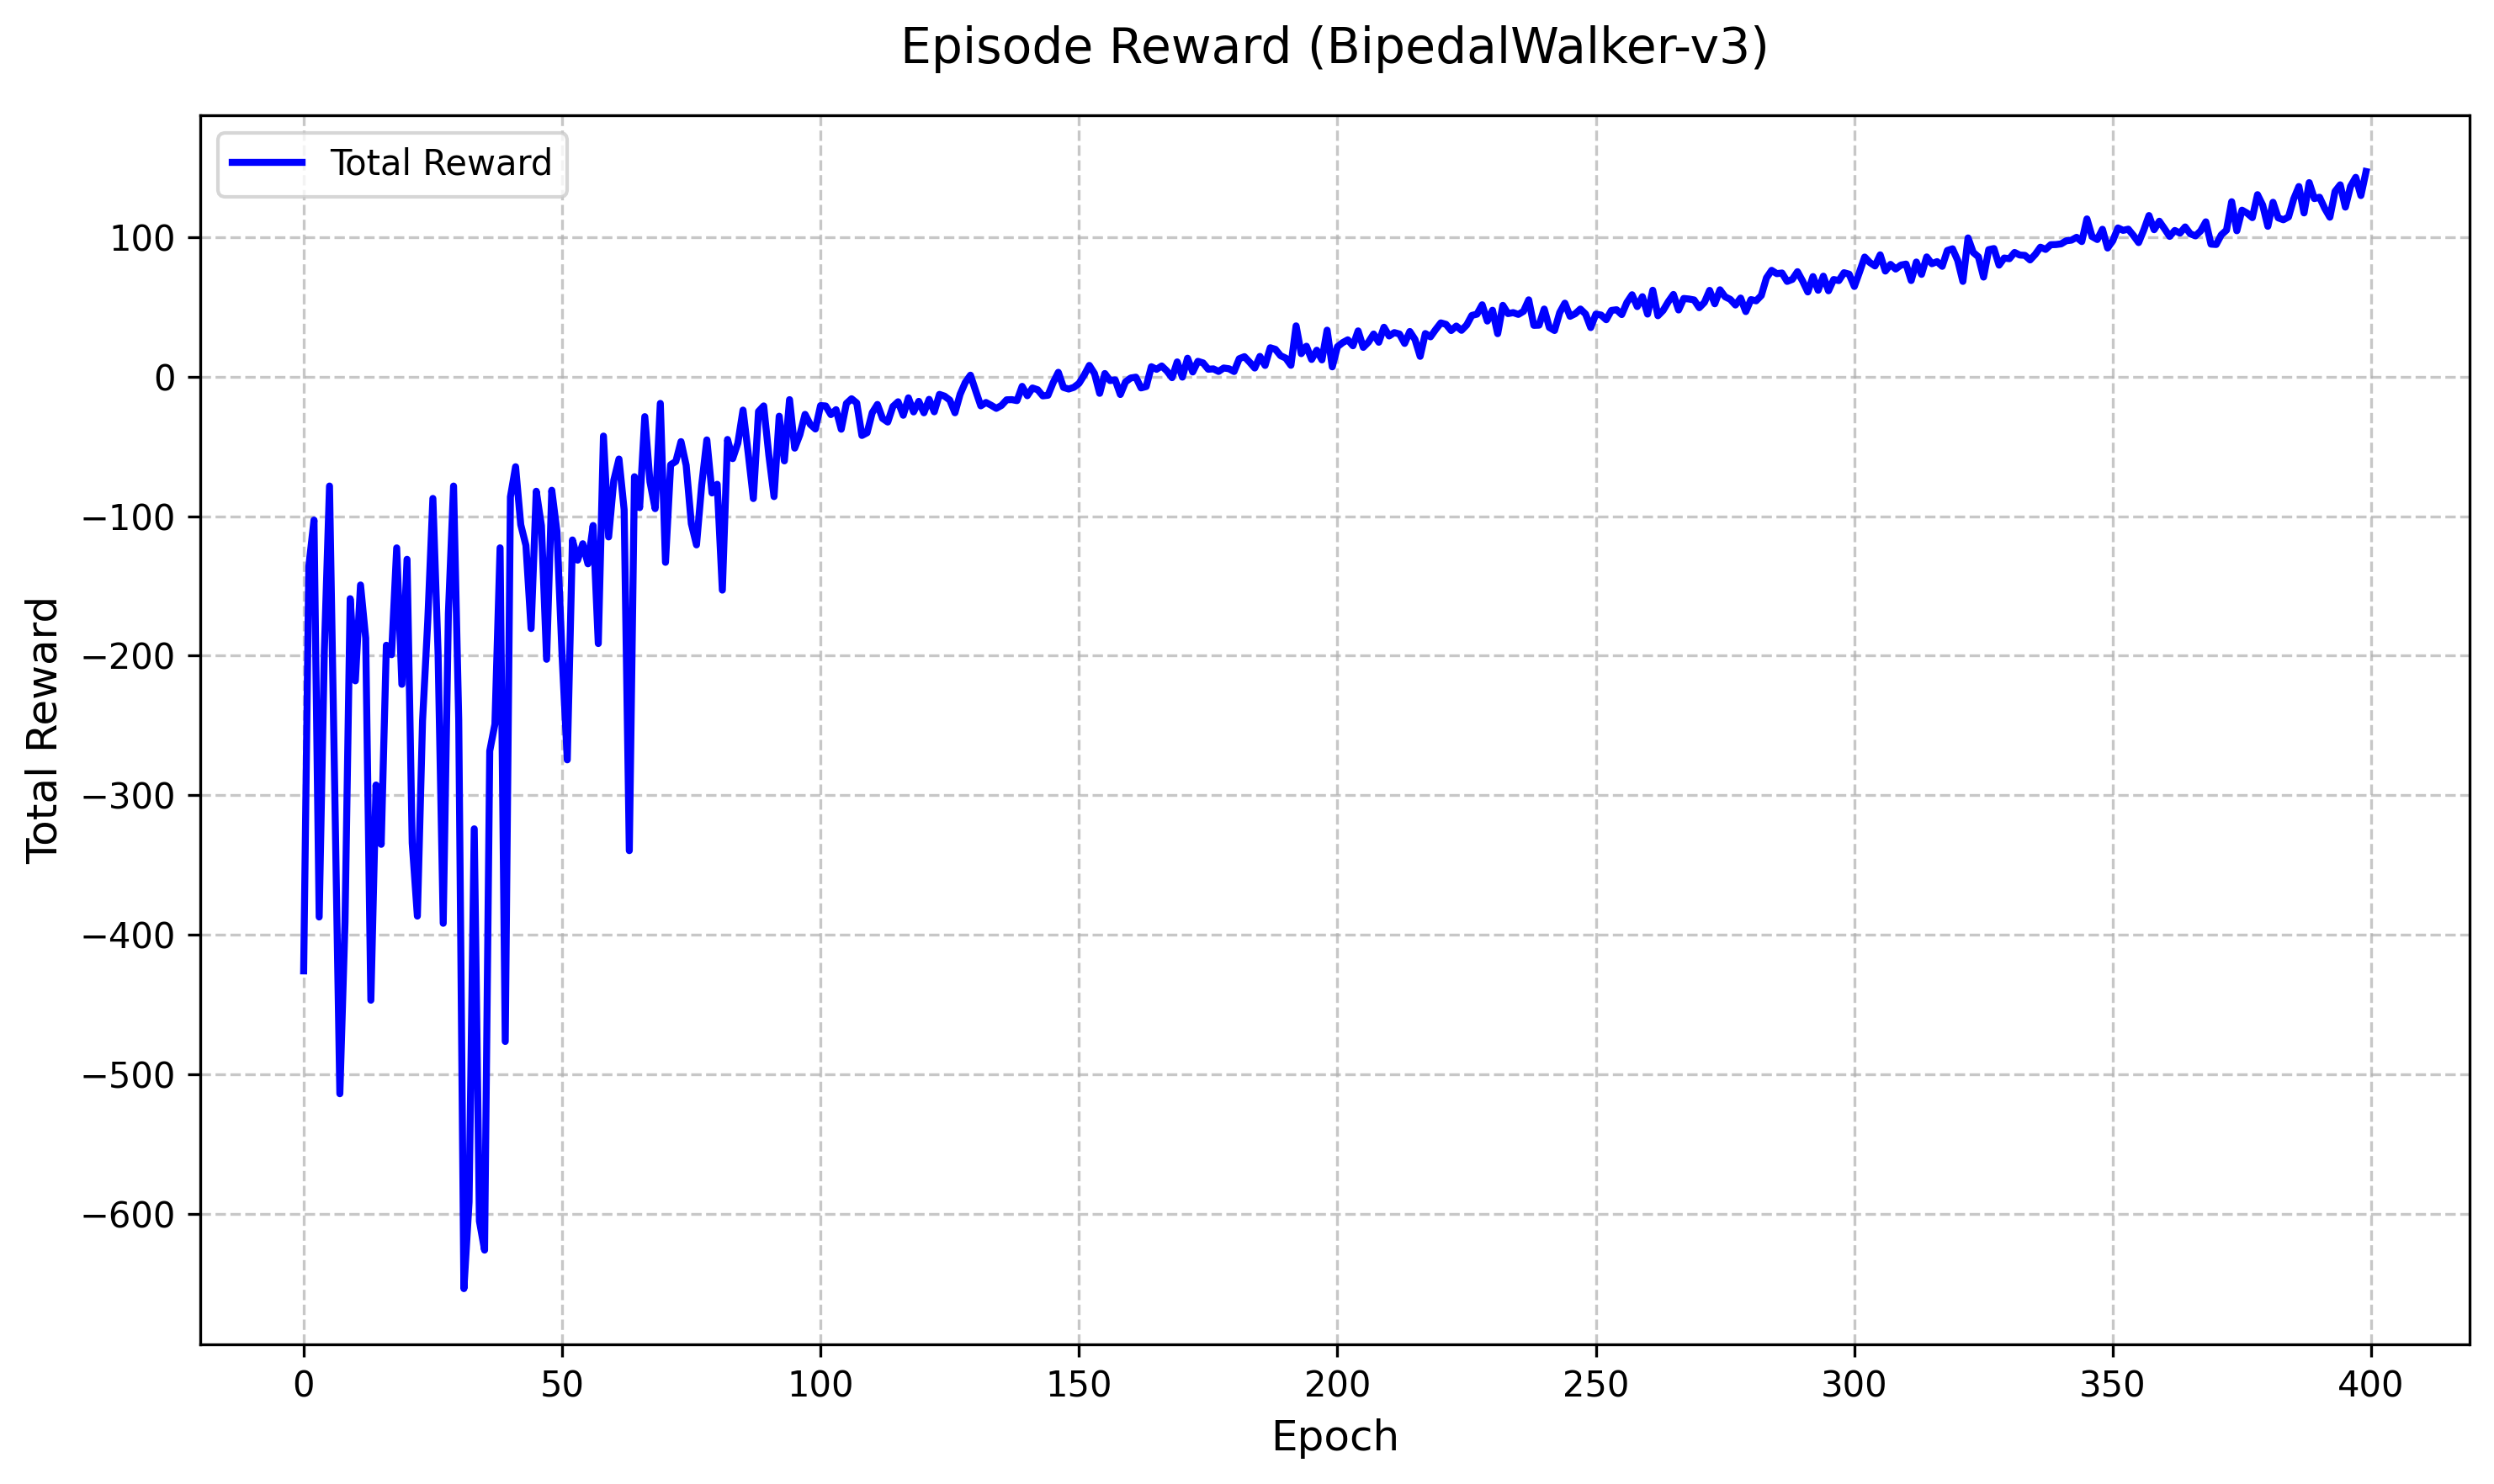
\includegraphics[width=\linewidth]{img/04-replay-batch-combo--bw-final-02-balanced-replay-explore-400-seed12--reward.png}
        \caption{Reward}
    \end{subfigure}\hfill
    \begin{subfigure}{0.31\textwidth}
        \centering
        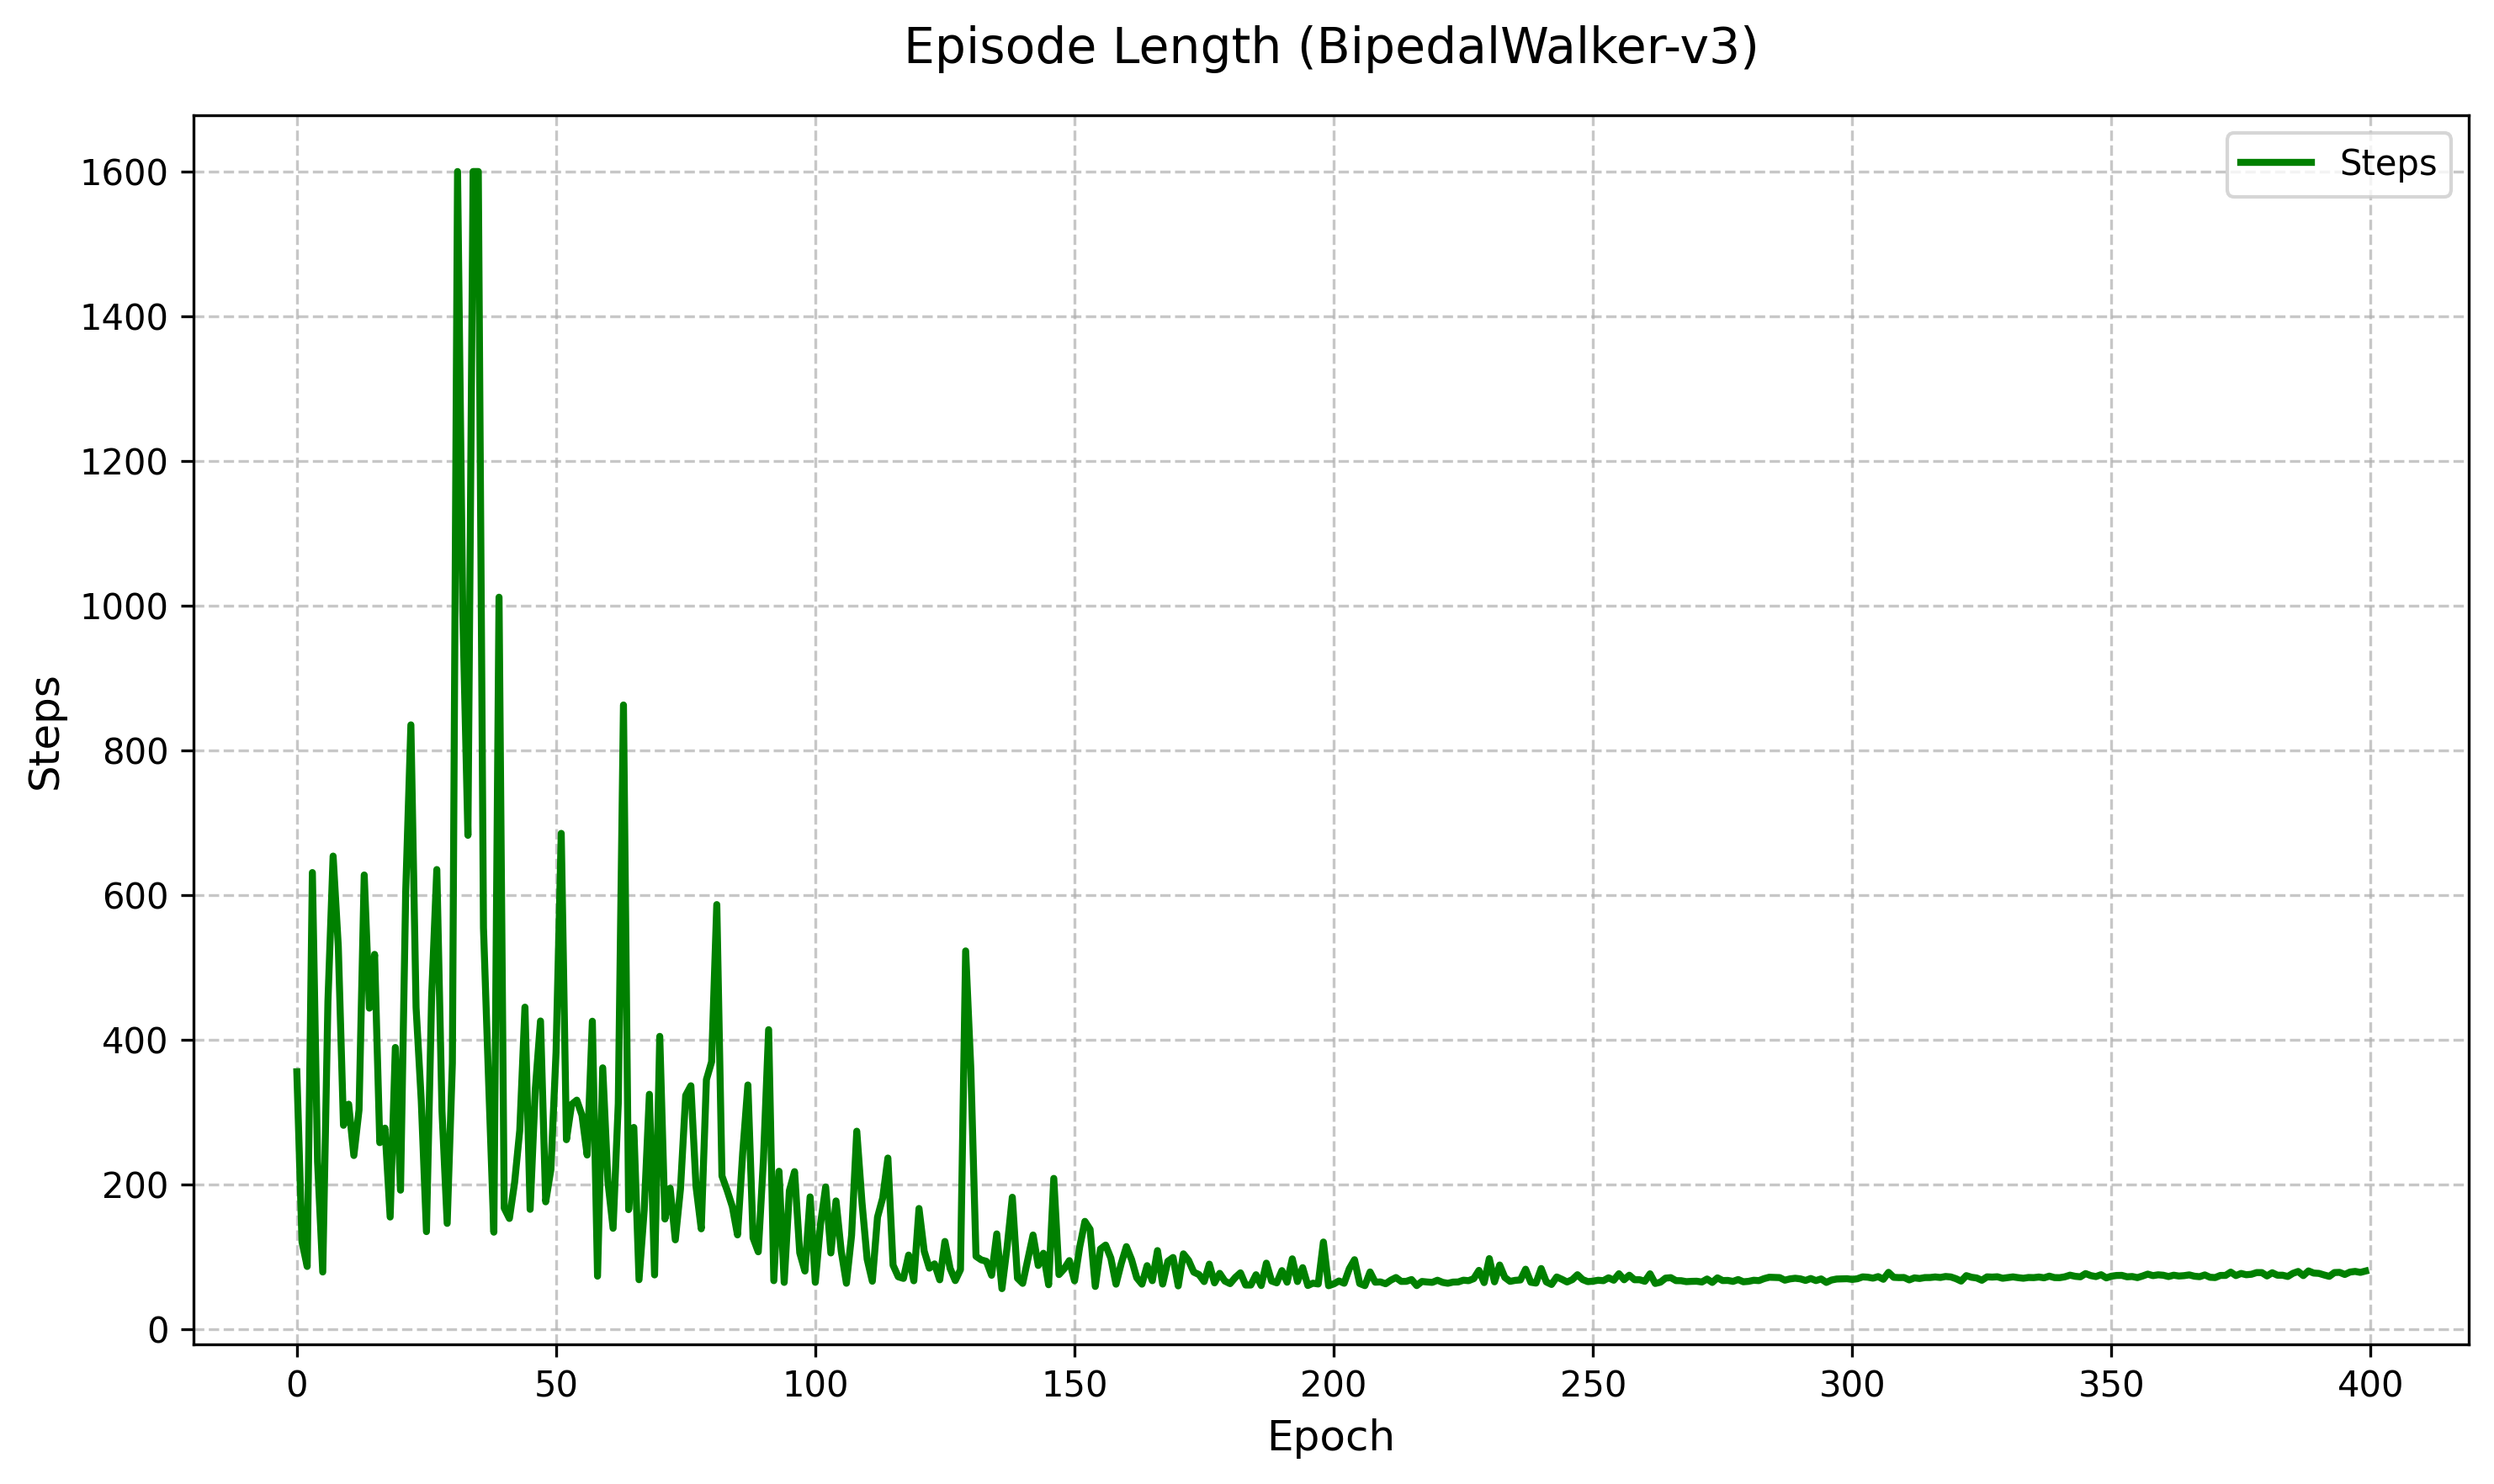
\includegraphics[width=\linewidth]{img/04-replay-batch-combo--bw-final-02-balanced-replay-explore-400-seed12--length.png}
        \caption{Length}
    \end{subfigure}\hfill
    \begin{subfigure}{0.31\textwidth}
        \centering
        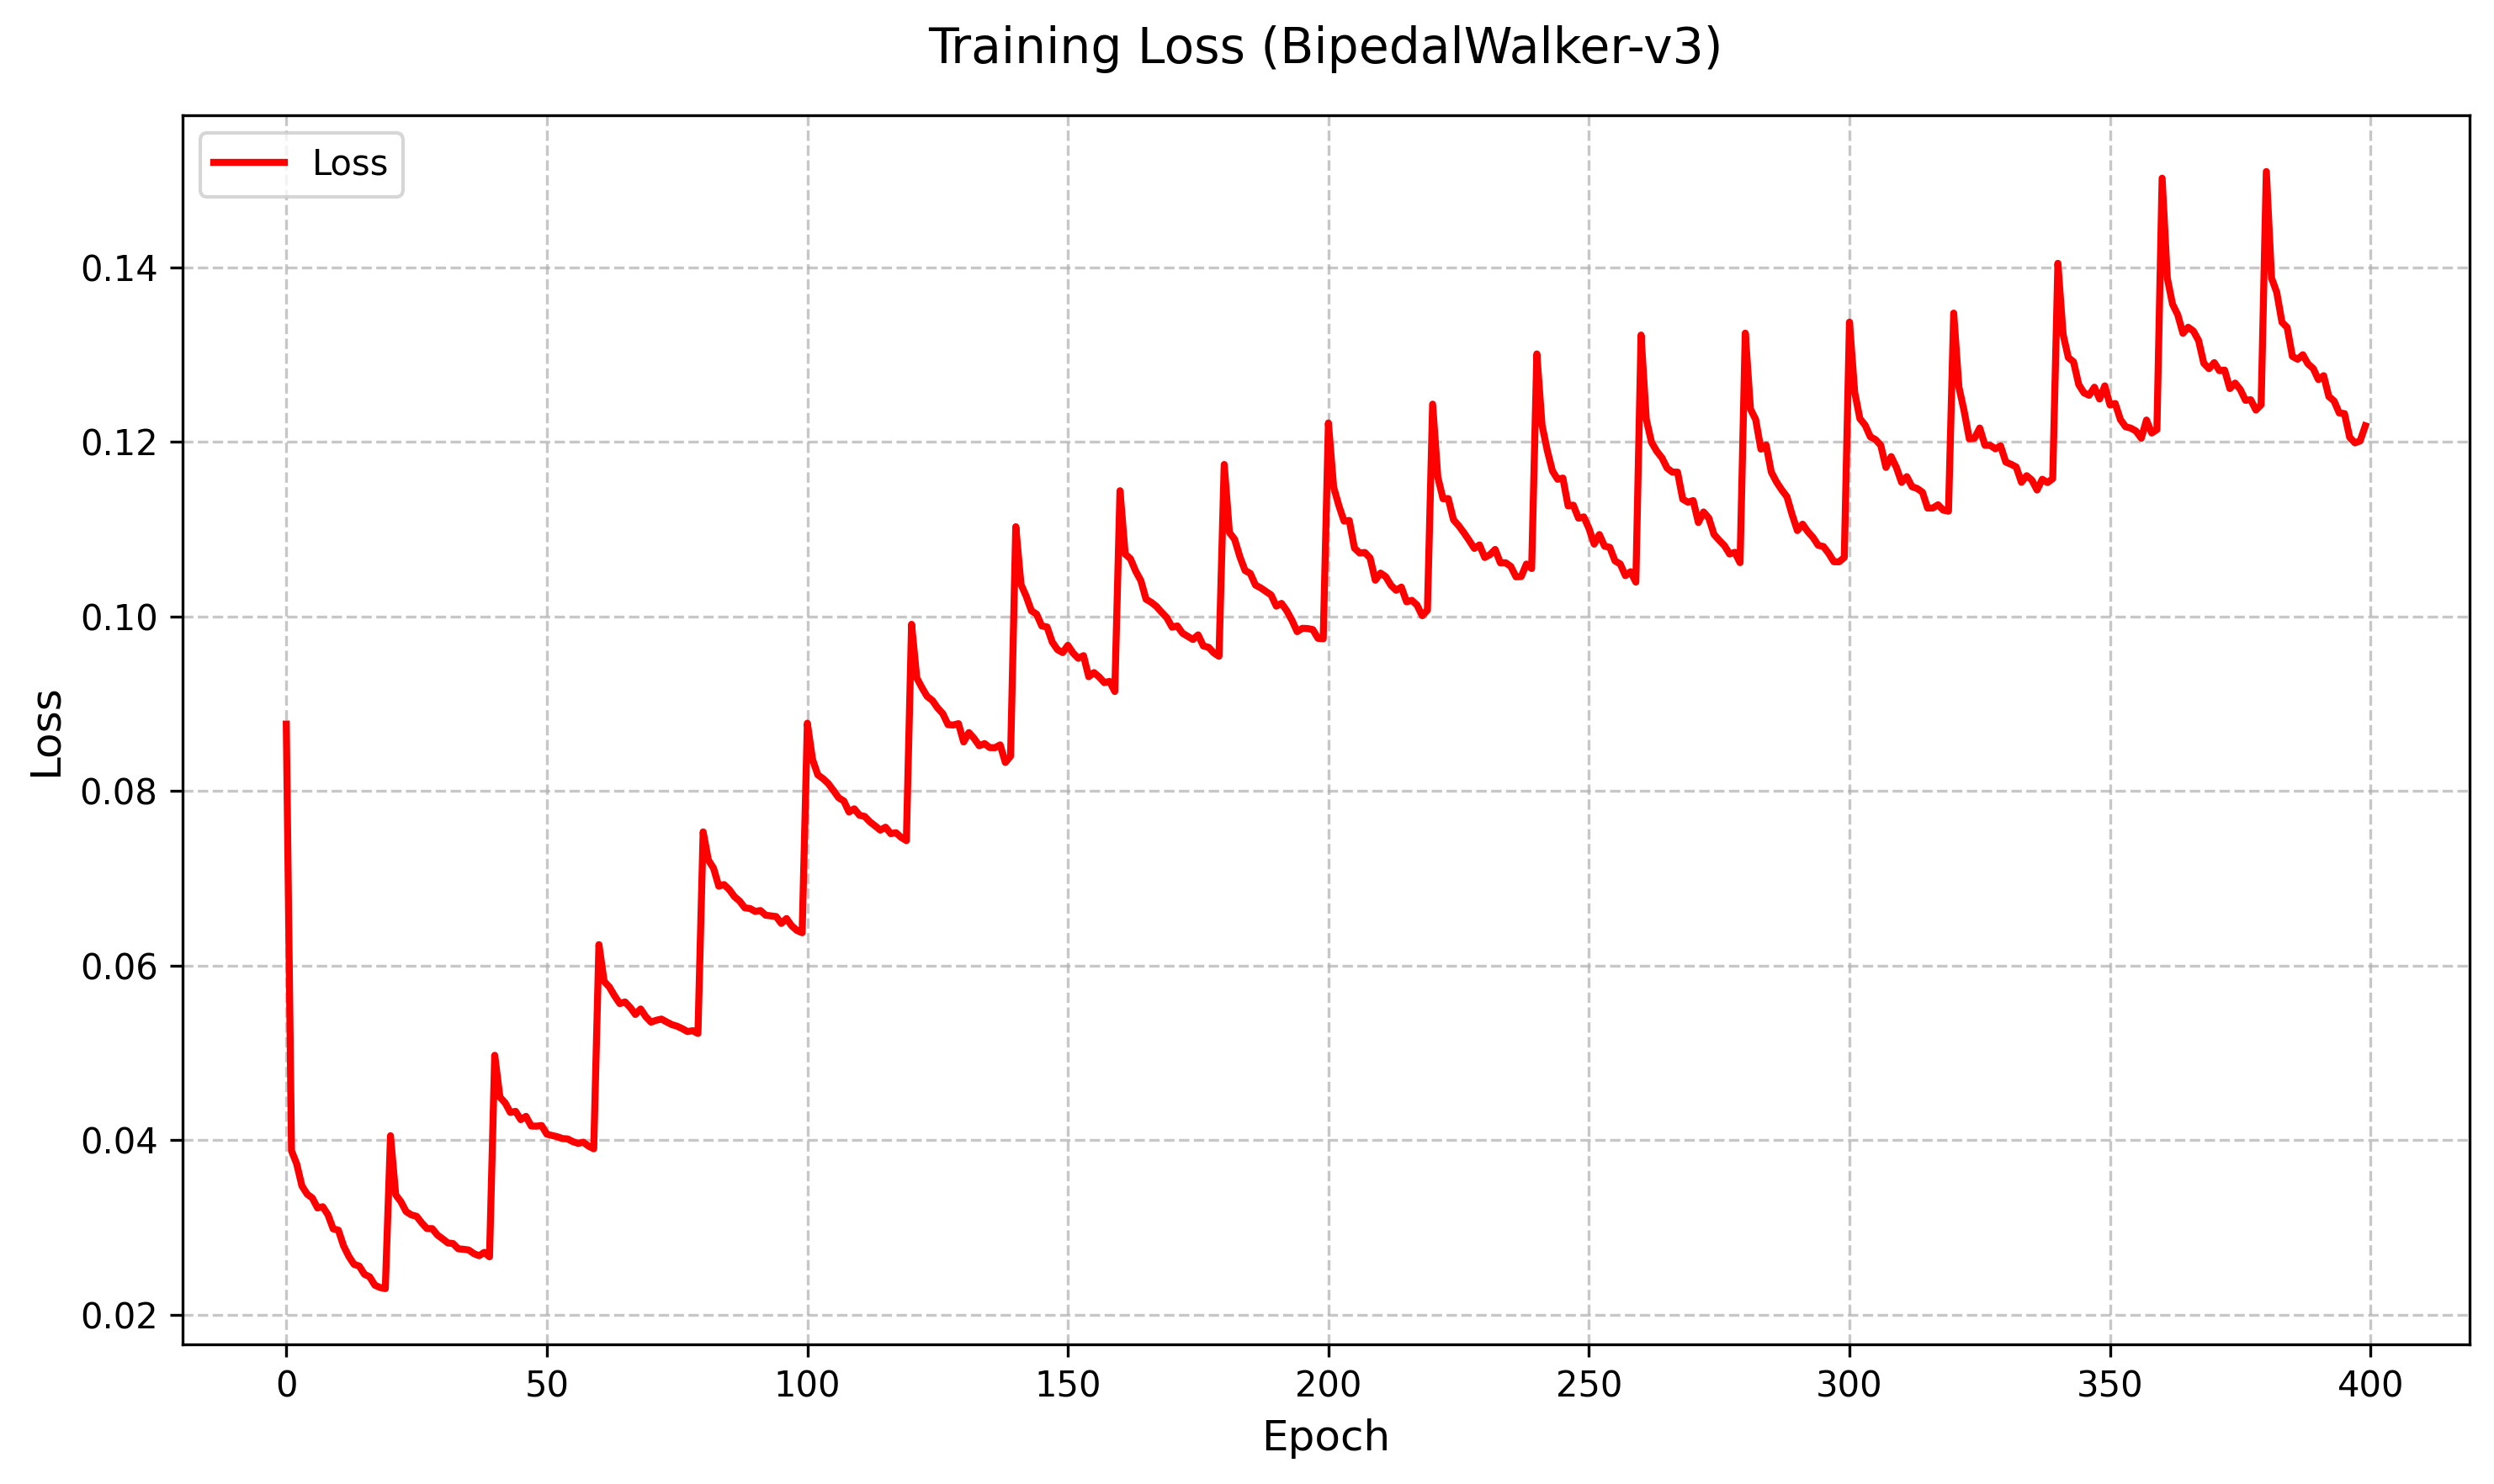
\includegraphics[width=\linewidth]{img/04-replay-batch-combo--bw-final-02-balanced-replay-explore-400-seed12--loss.png}
        \caption{Loss}
    \end{subfigure}
    \caption{Category 04: Replay Buffer and Batch Size Combo}
\end{figure}

% 05 - Gamma
\begin{figure}[H]
    \centering
    \begin{subfigure}{0.31\textwidth}
        \centering
        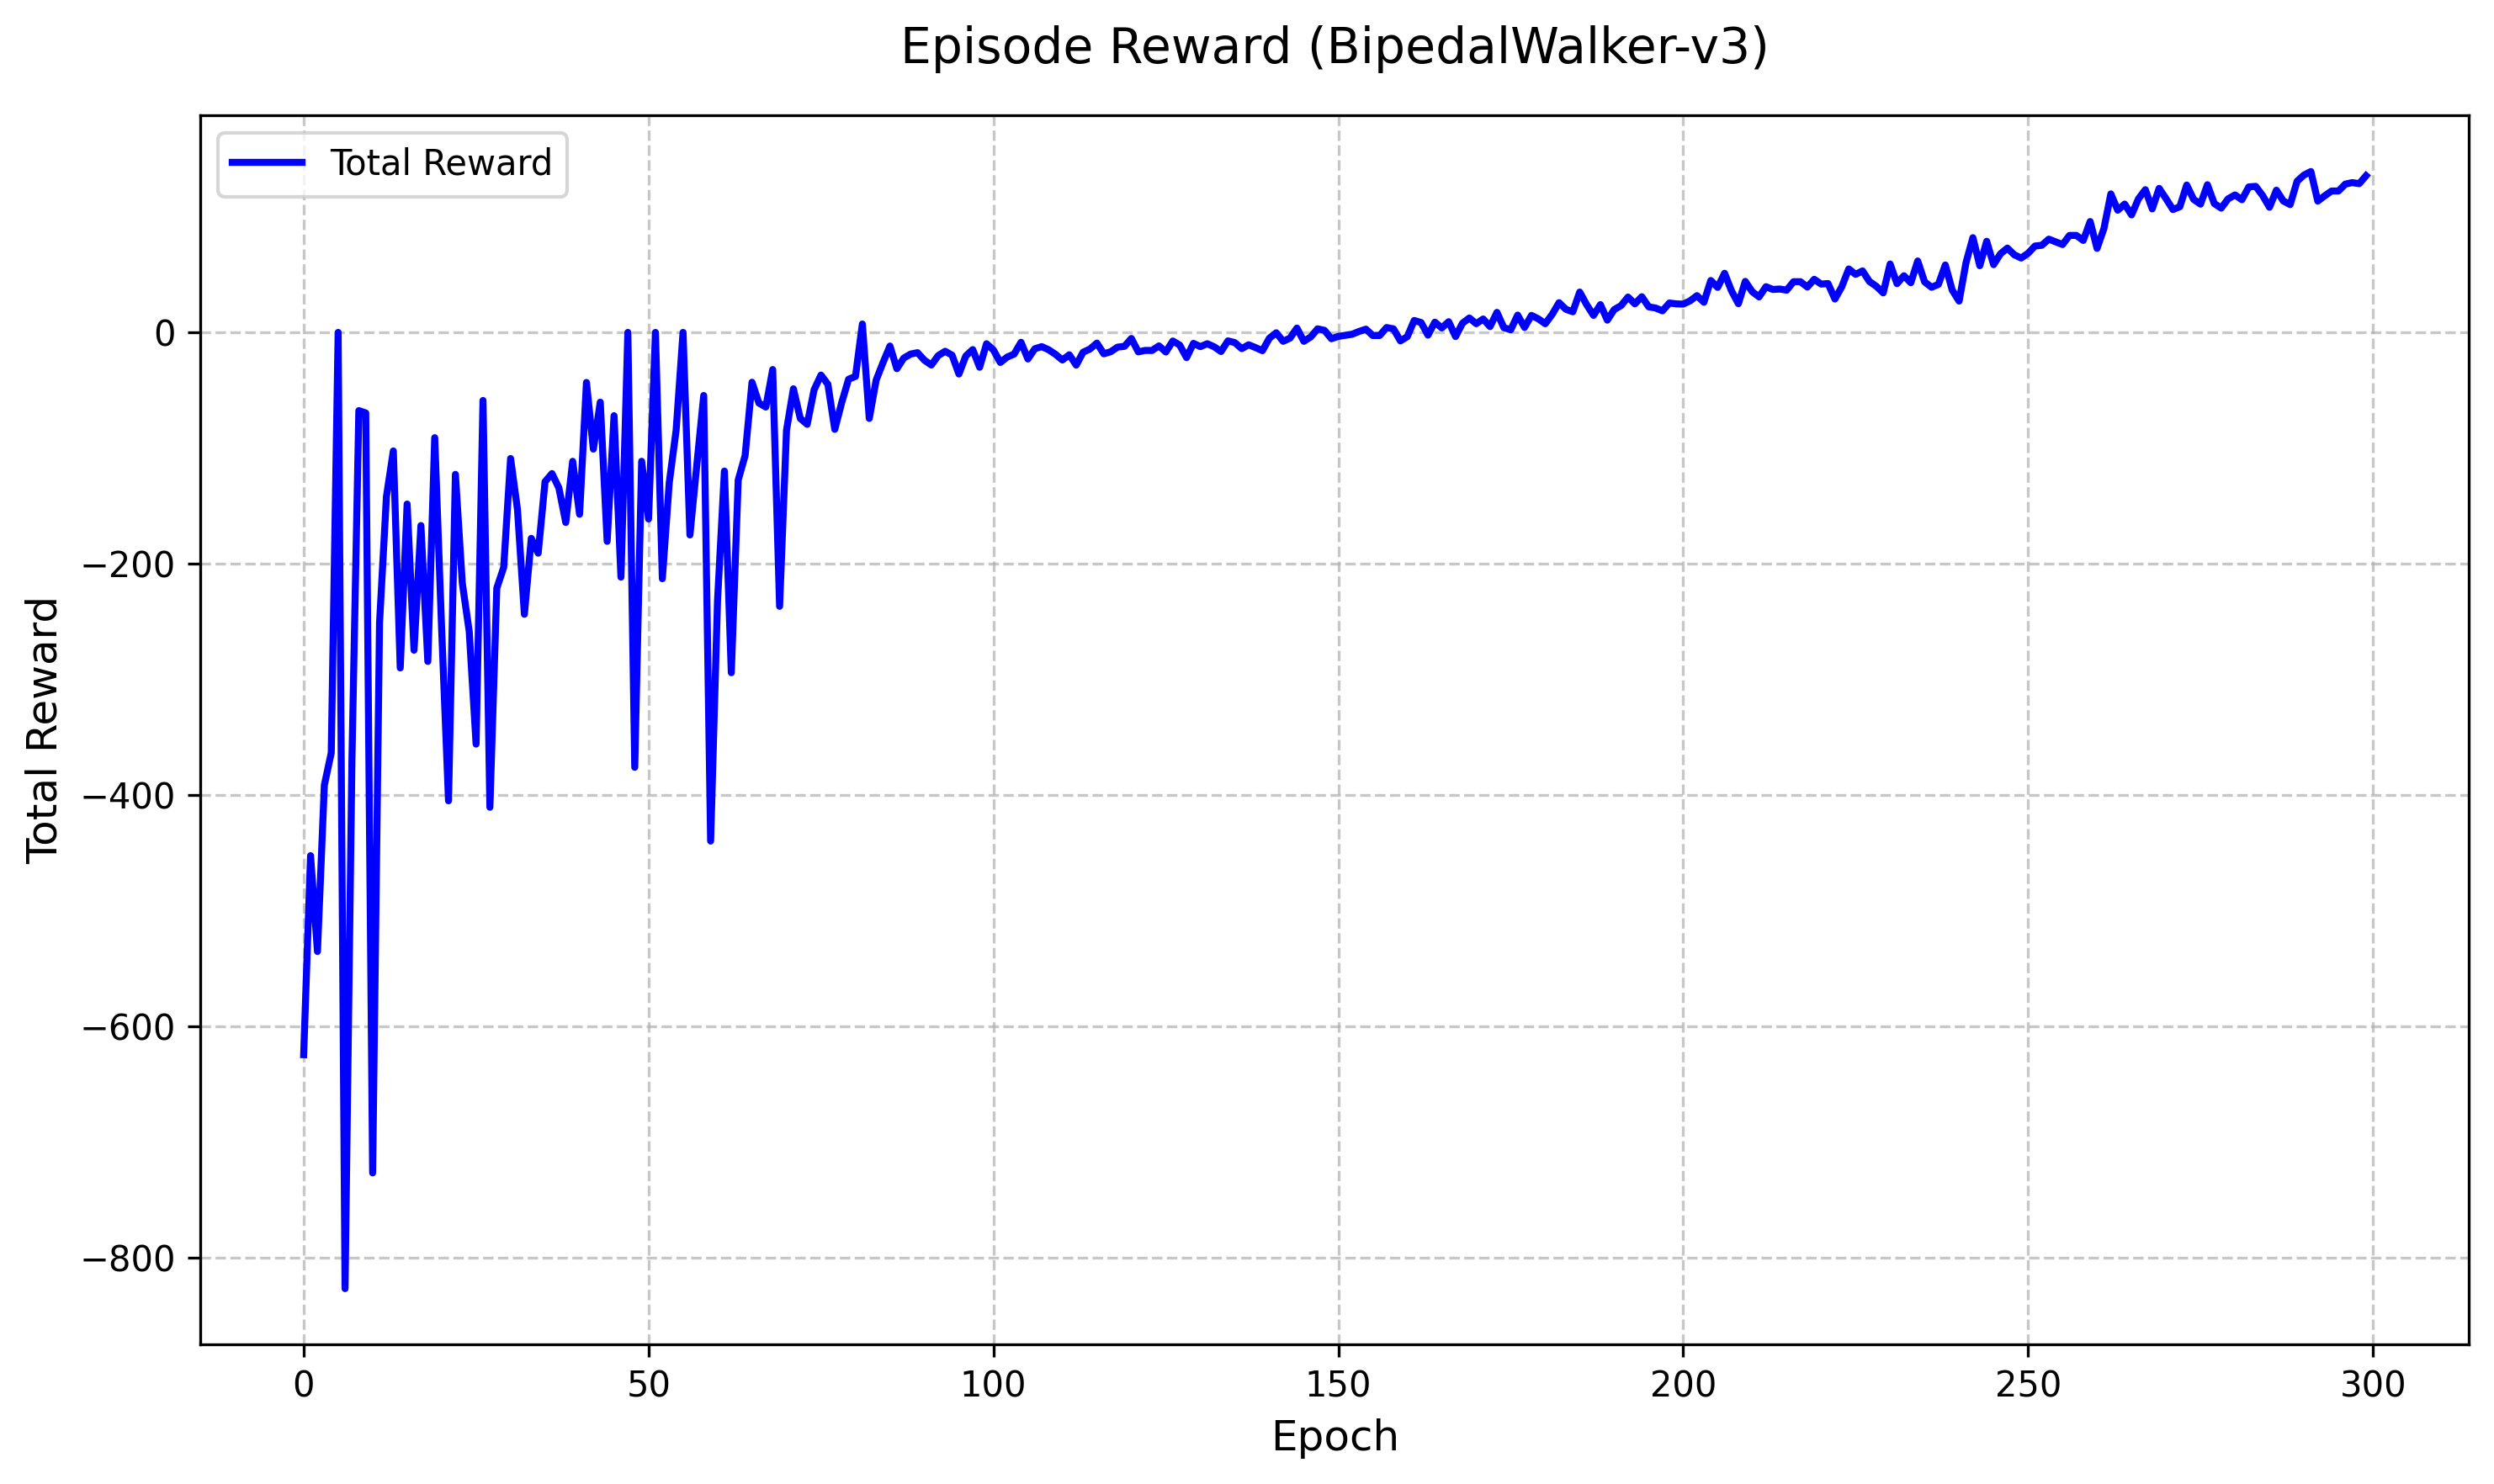
\includegraphics[width=\linewidth]{img/05-gamma--bw-07-gamma-097-ablation-300--reward.png}
        \caption{Reward}
    \end{subfigure}\hfill
    \begin{subfigure}{0.31\textwidth}
        \centering
        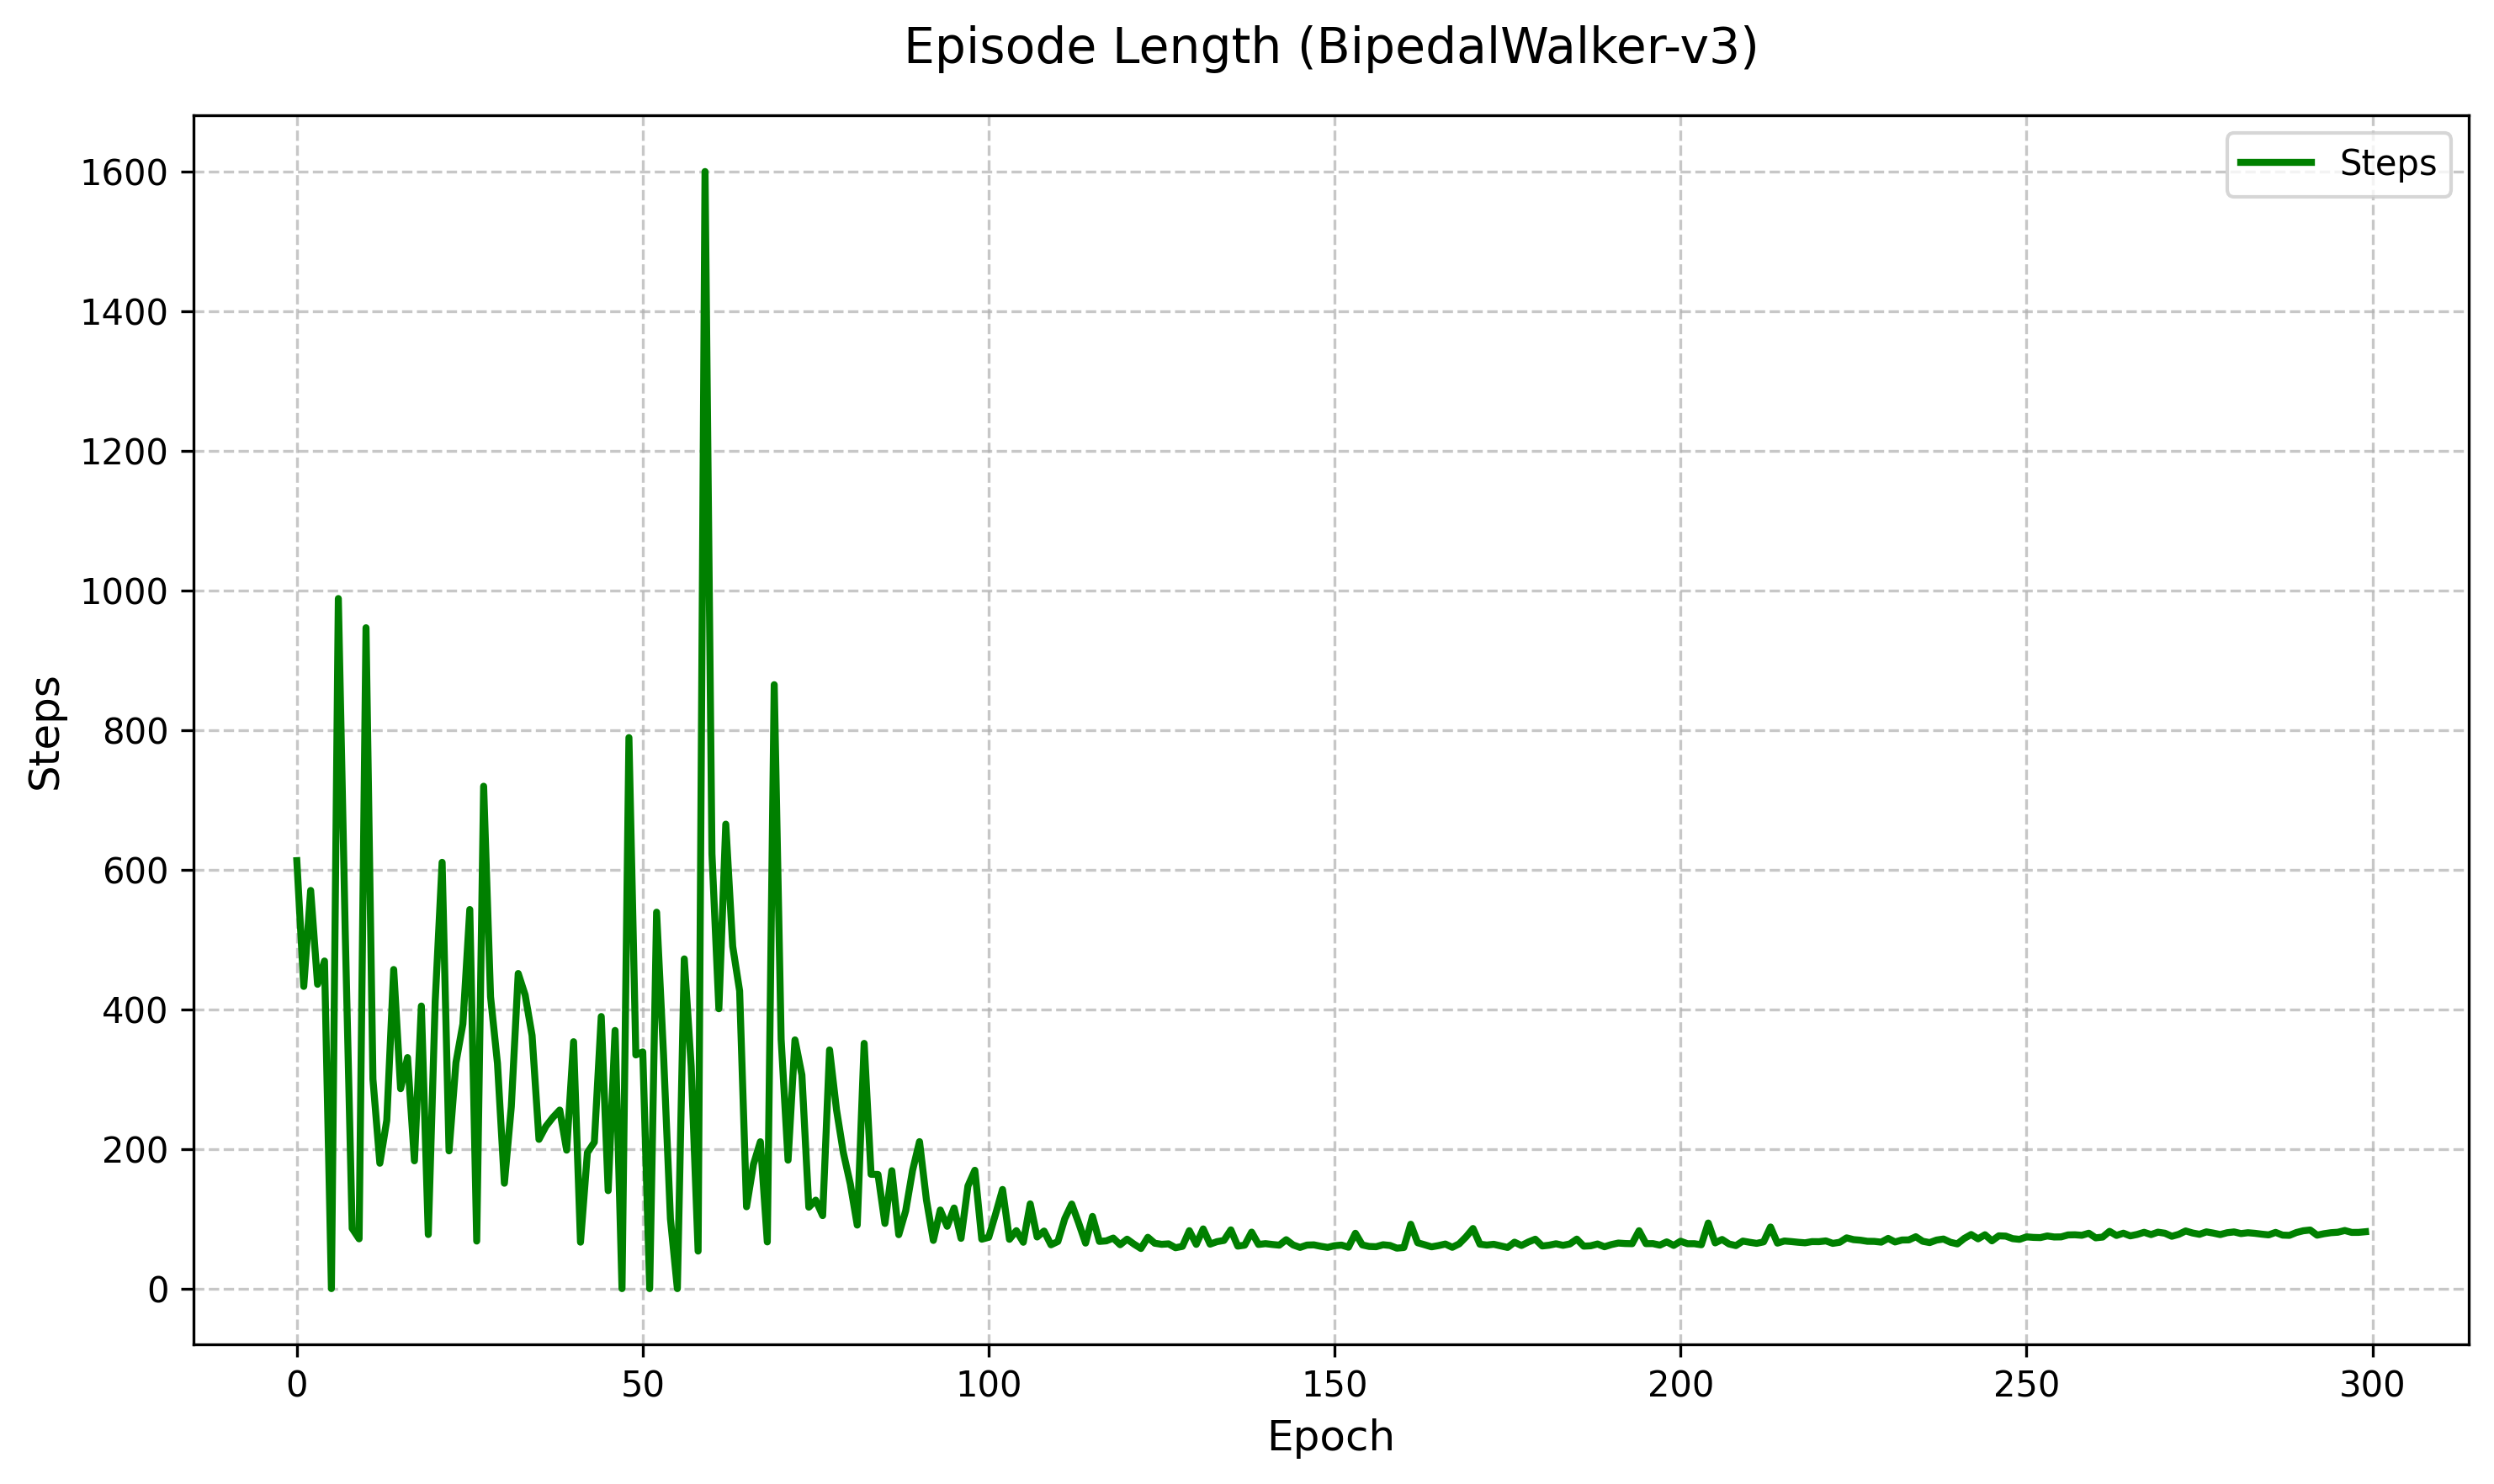
\includegraphics[width=\linewidth]{img/05-gamma--bw-07-gamma-097-ablation-300--length.png}
        \caption{Length}
    \end{subfigure}\hfill
    \begin{subfigure}{0.31\textwidth}
        \centering
        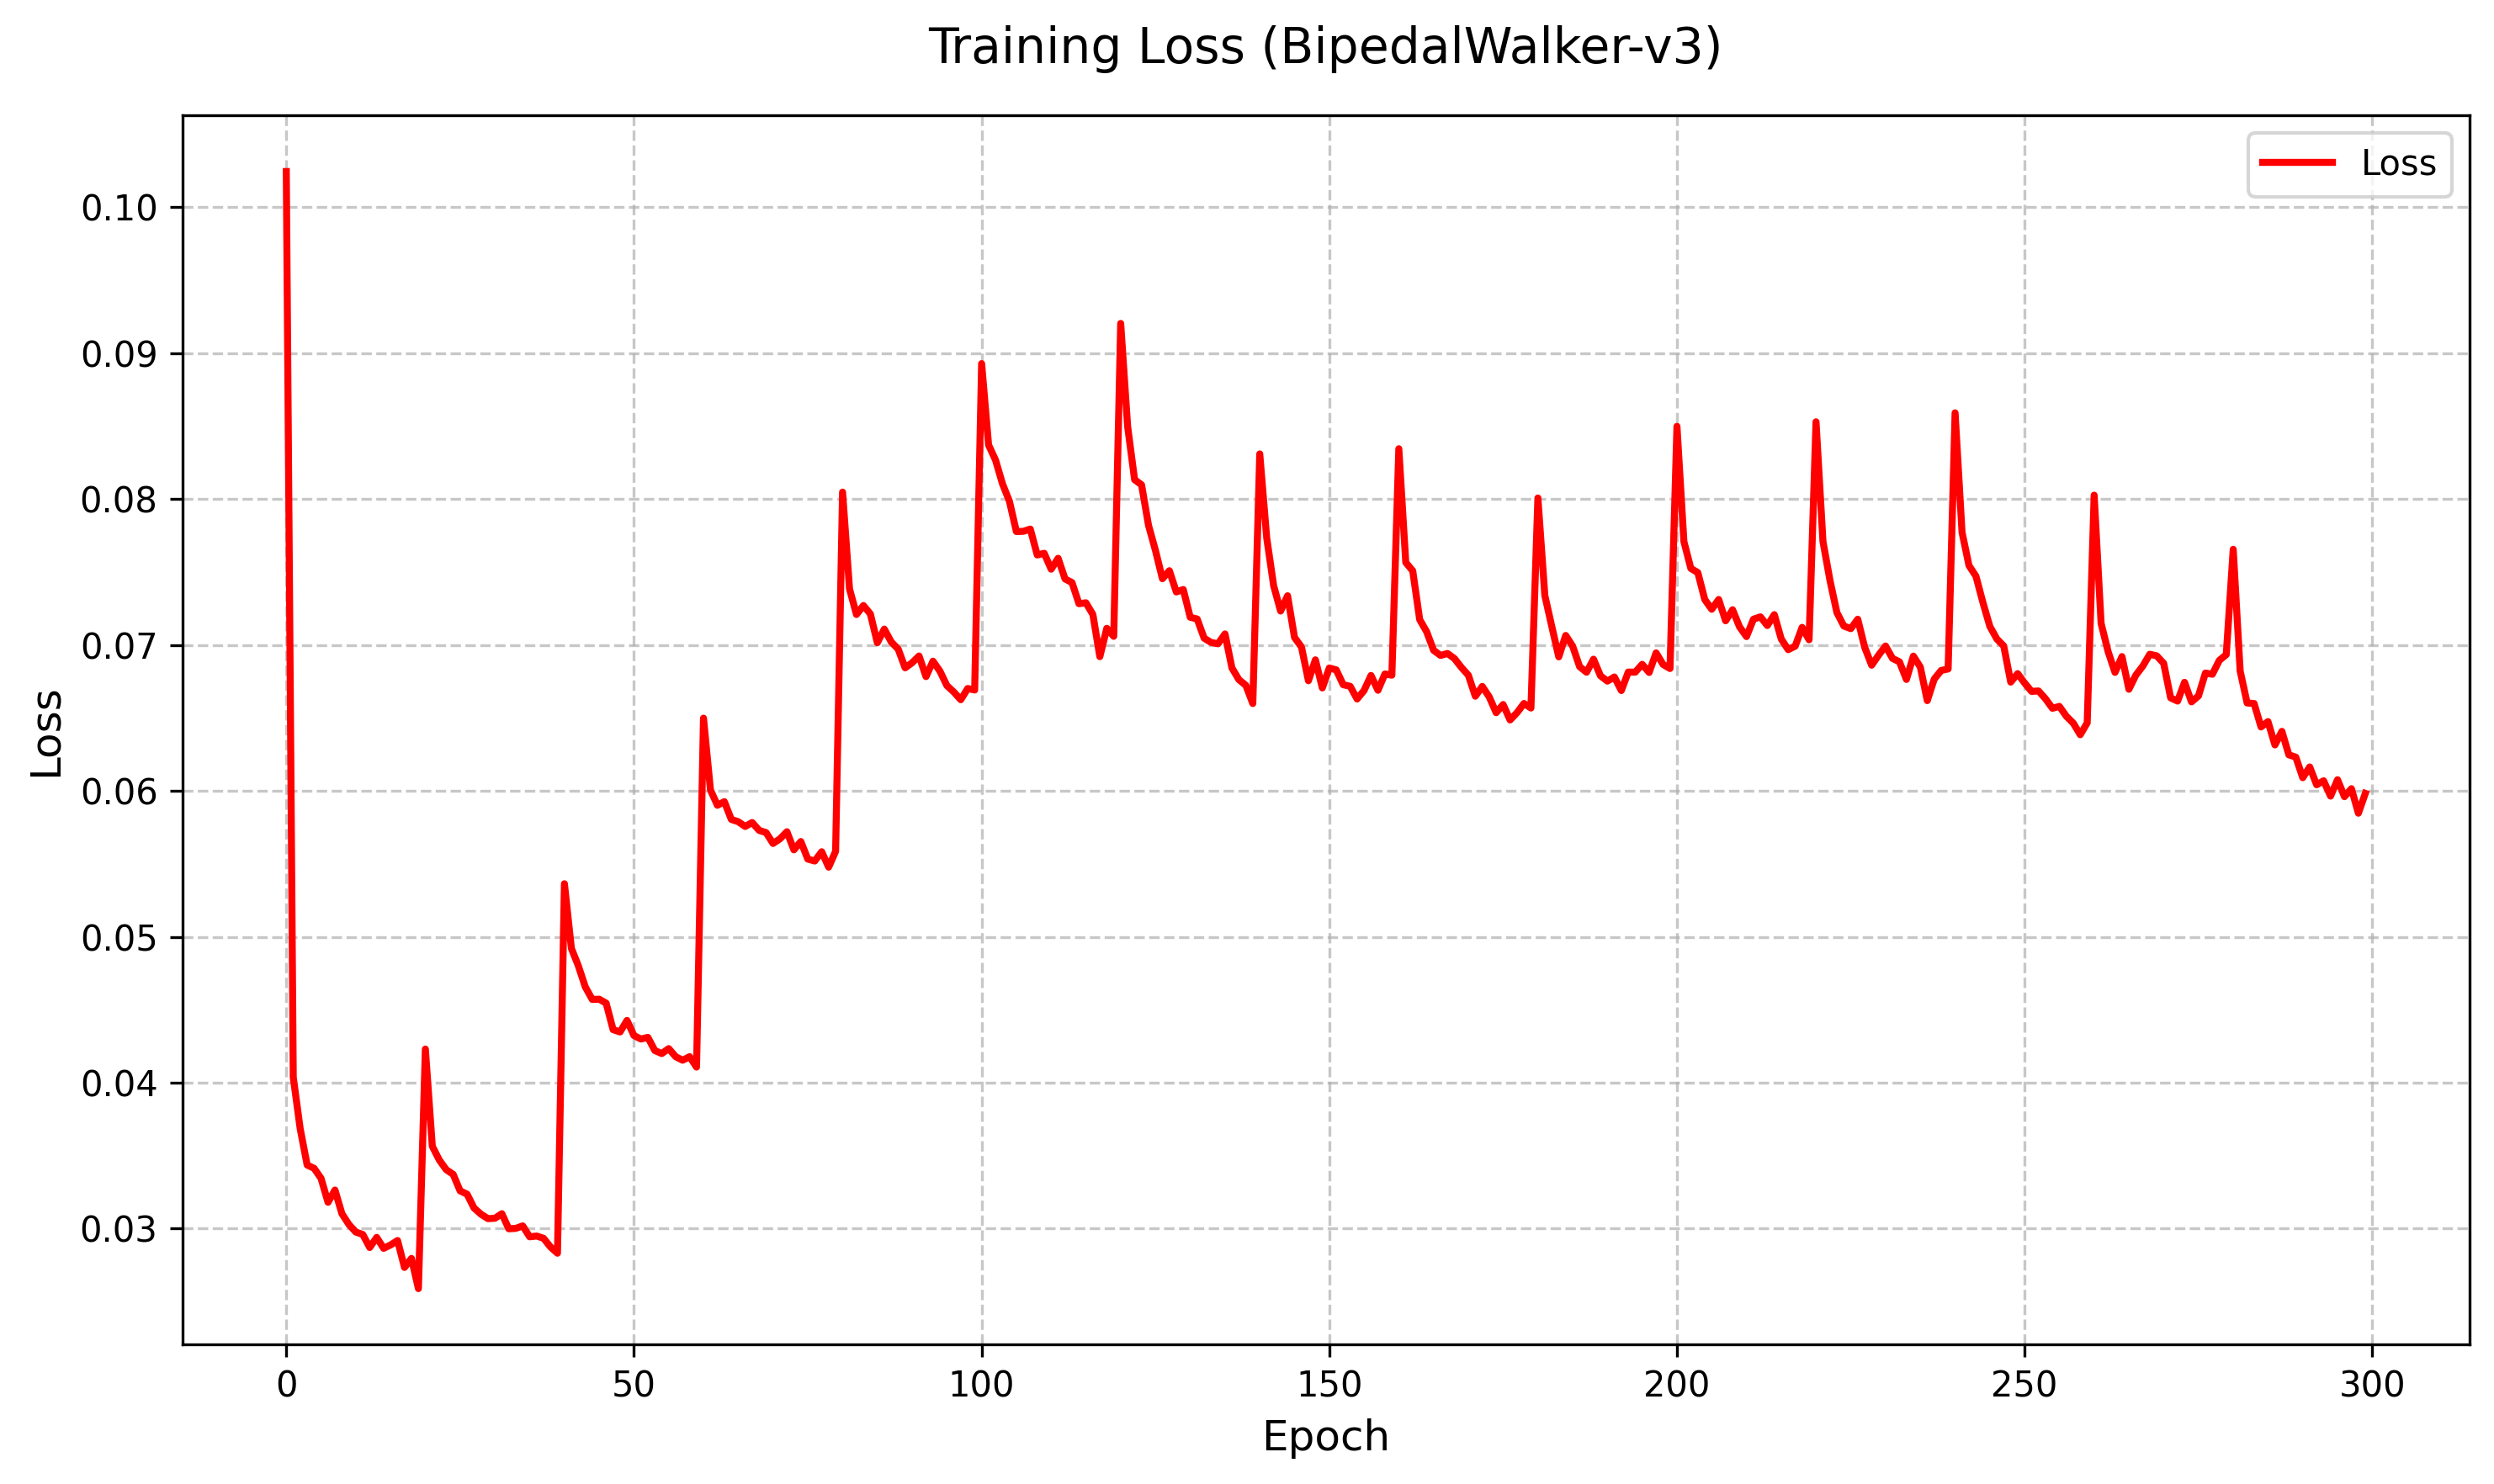
\includegraphics[width=\linewidth]{img/05-gamma--bw-07-gamma-097-ablation-300--loss.png}
        \caption{Loss}
    \end{subfigure}
    \caption{Category 05: Gamma Discount Factor Ablation}
\end{figure}

% 06 - Boltzmann
\begin{figure}[H]
    \centering
    \begin{subfigure}{0.31\textwidth}
        \centering
        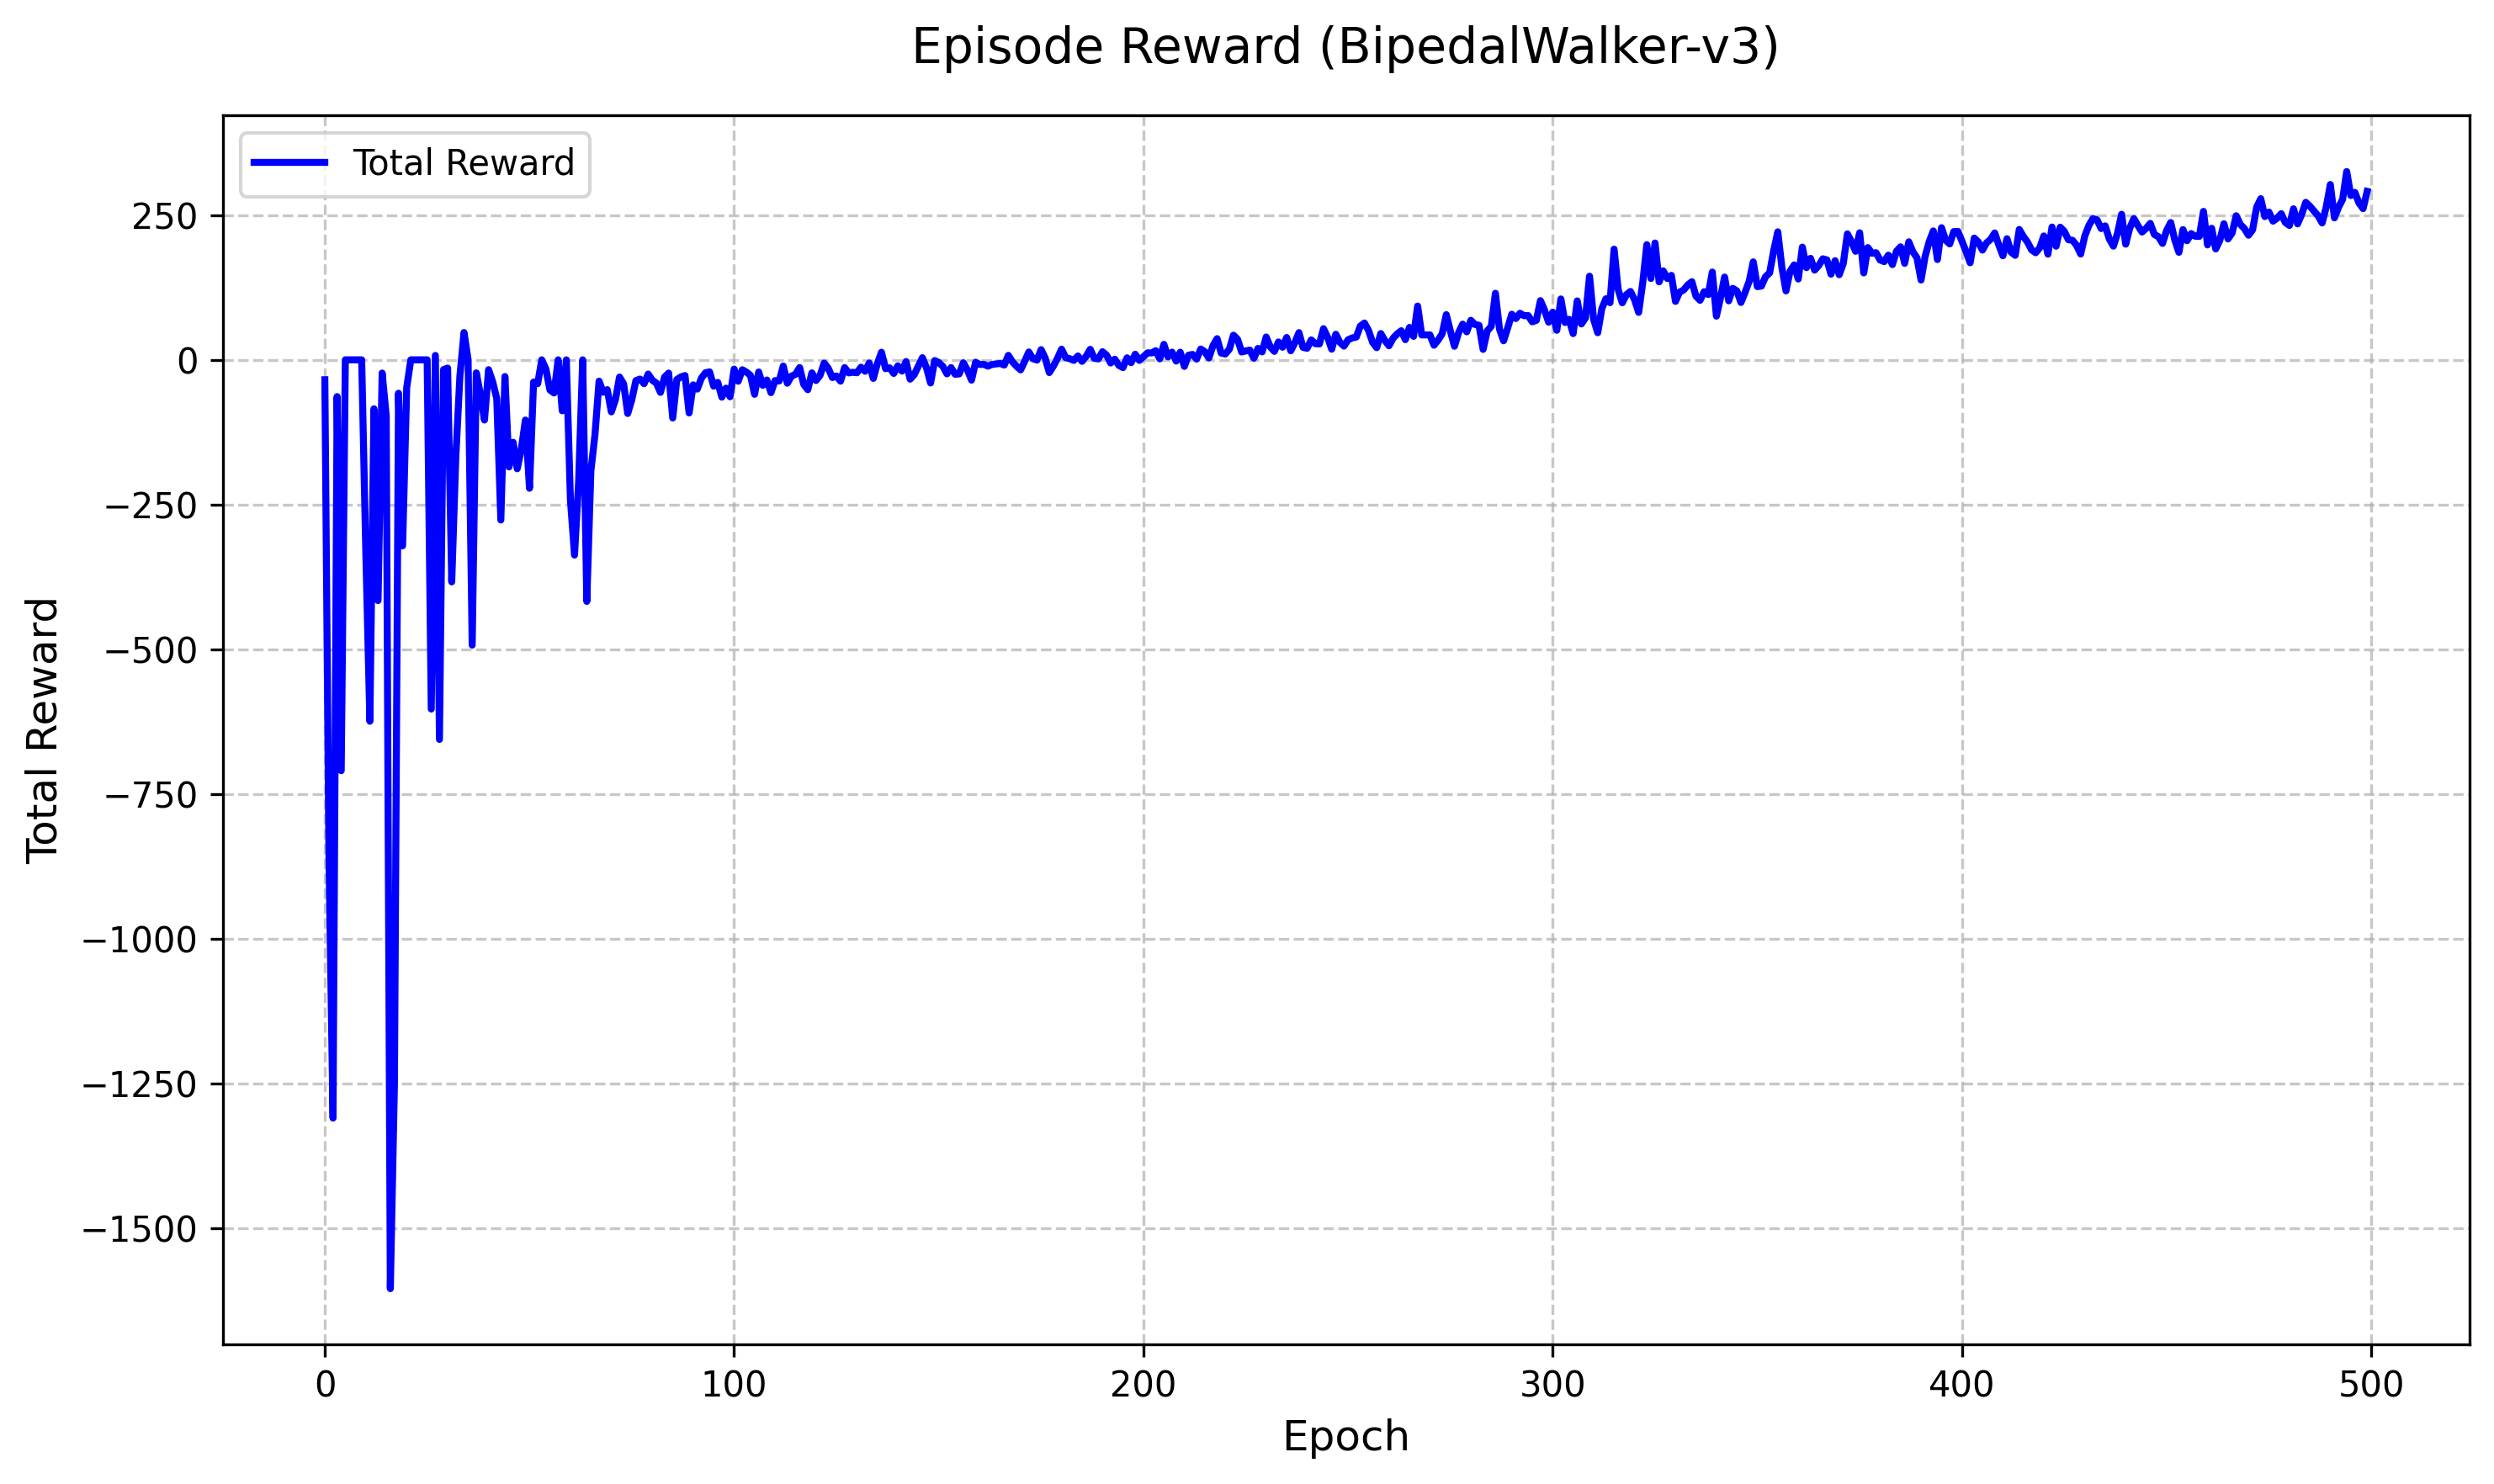
\includegraphics[width=\linewidth]{img/06-boltzmann--bw-boltzmann-final-01--reward.png}
        \caption{Reward}
    \end{subfigure}\hfill
    \begin{subfigure}{0.31\textwidth}
        \centering
        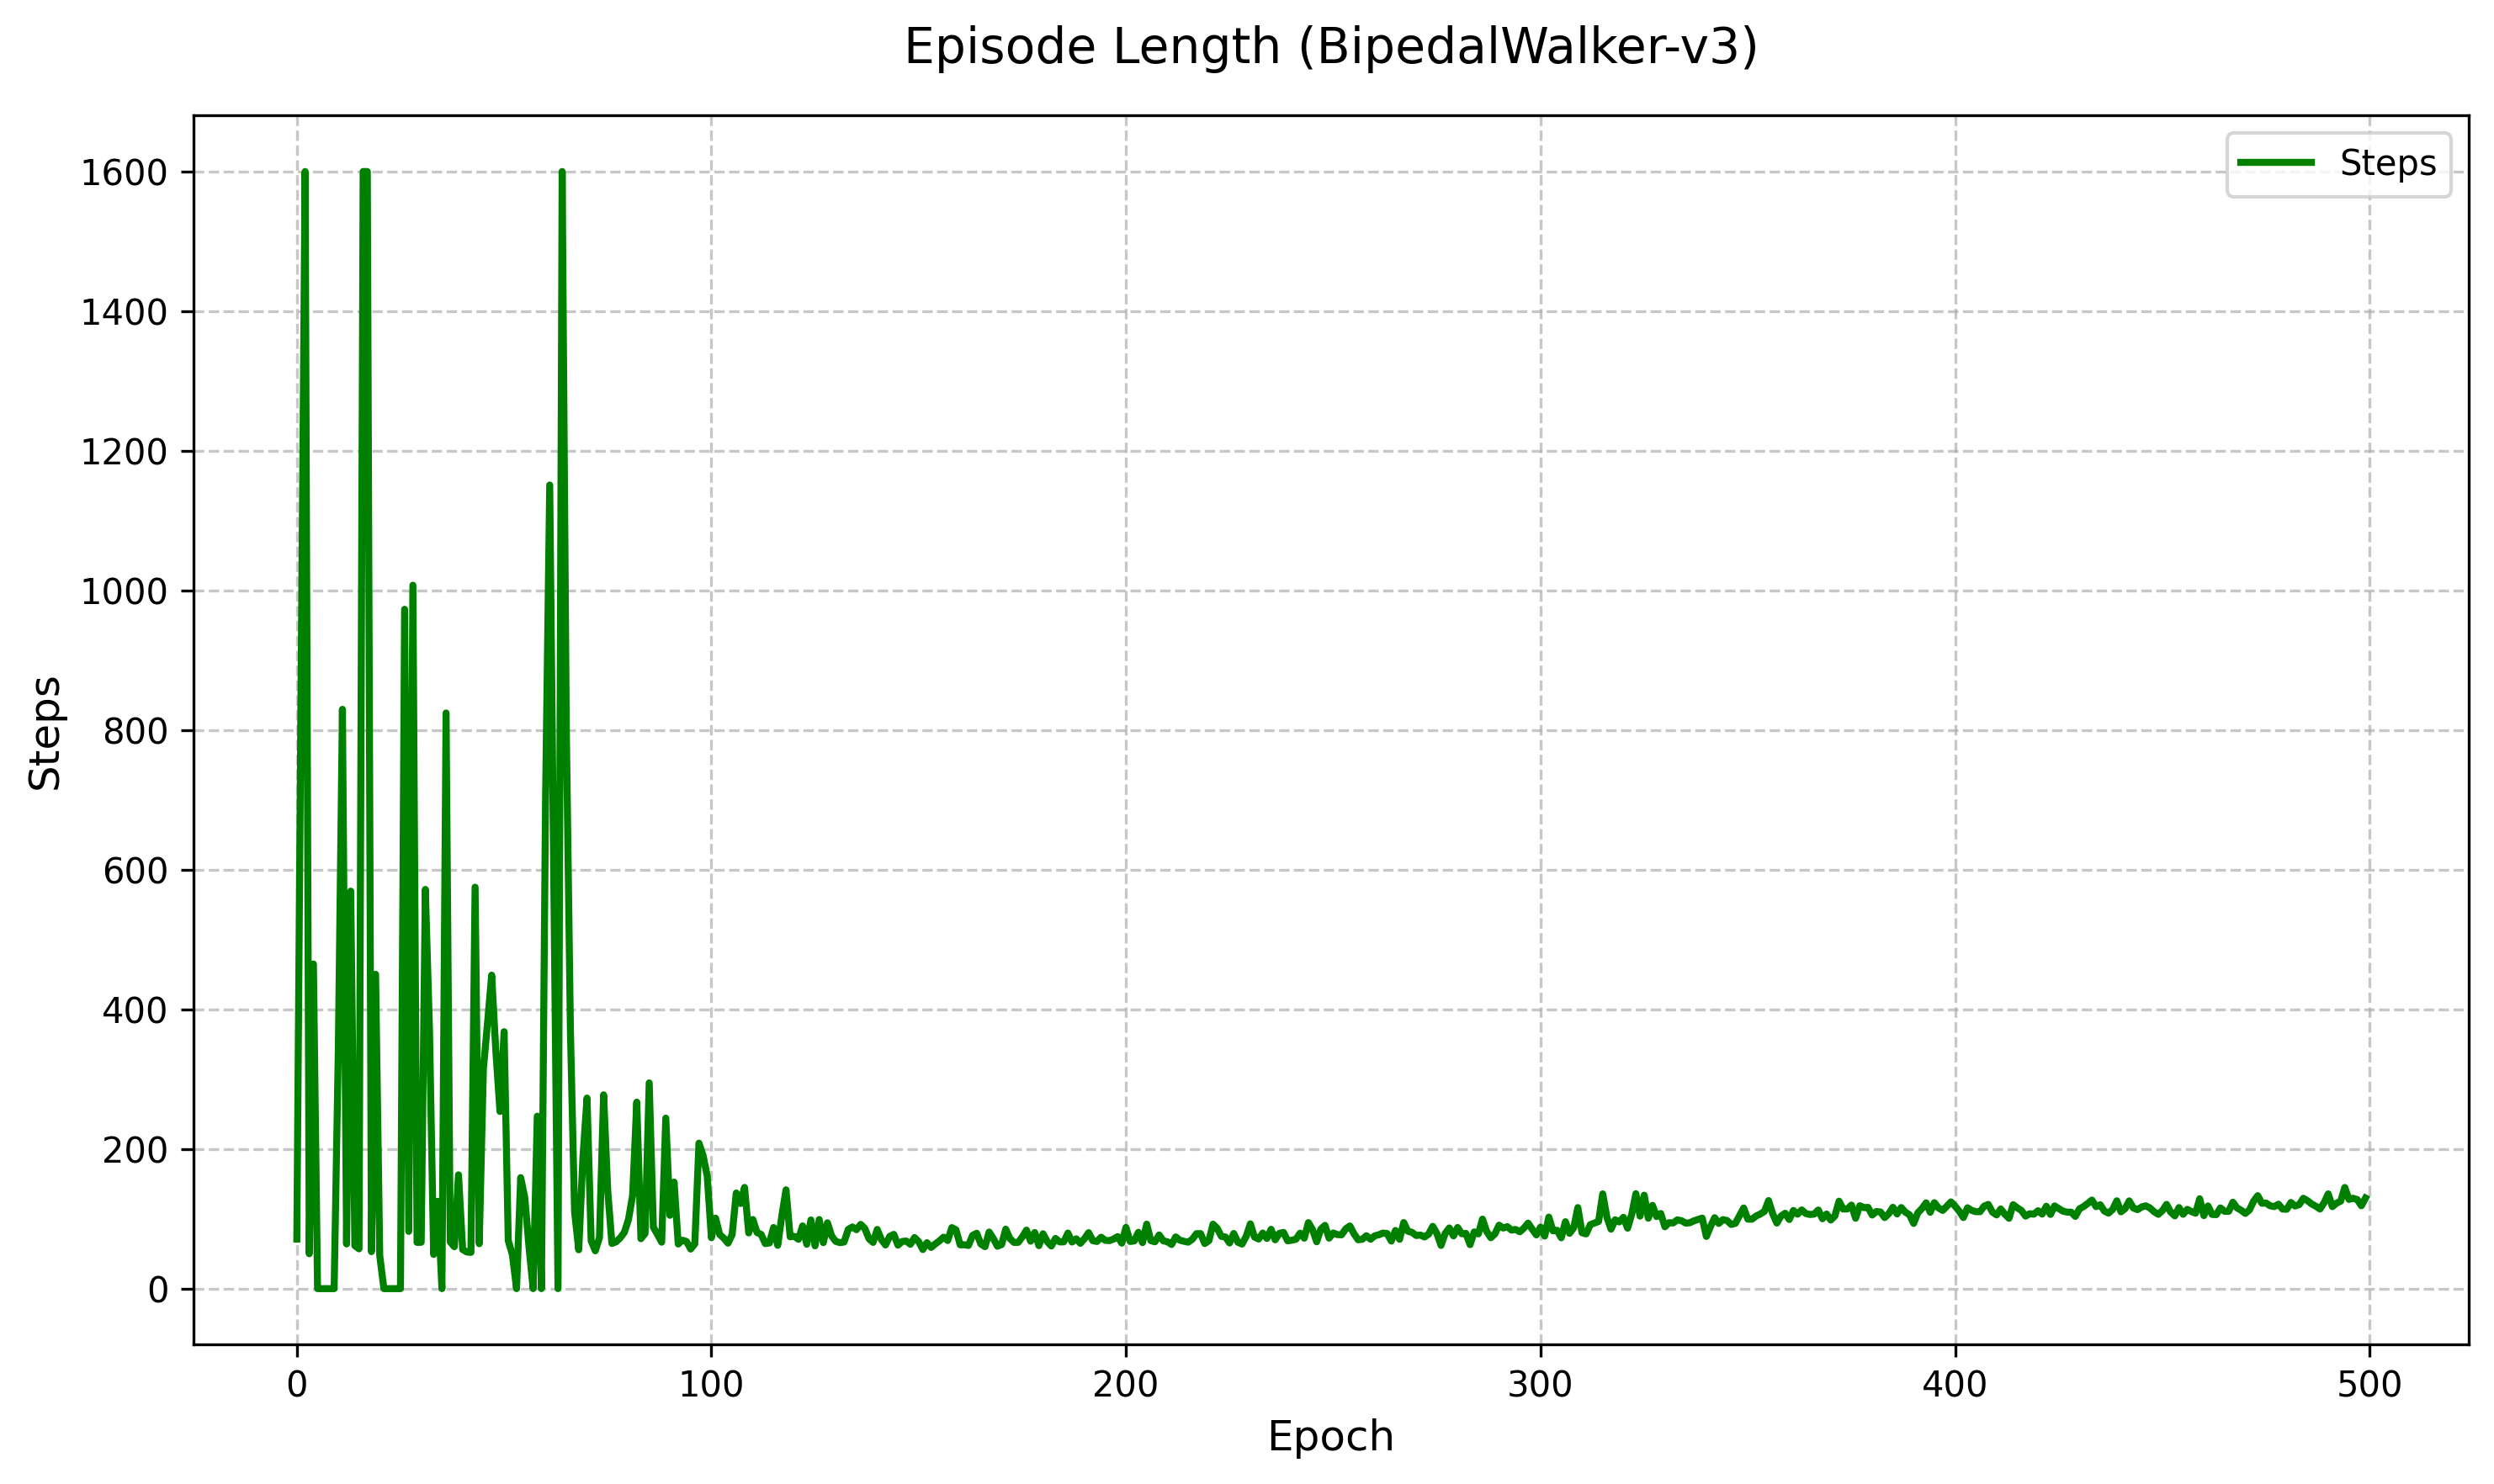
\includegraphics[width=\linewidth]{img/06-boltzmann--bw-boltzmann-final-01--length.png}
        \caption{Length}
    \end{subfigure}\hfill
    \begin{subfigure}{0.31\textwidth}
        \centering
        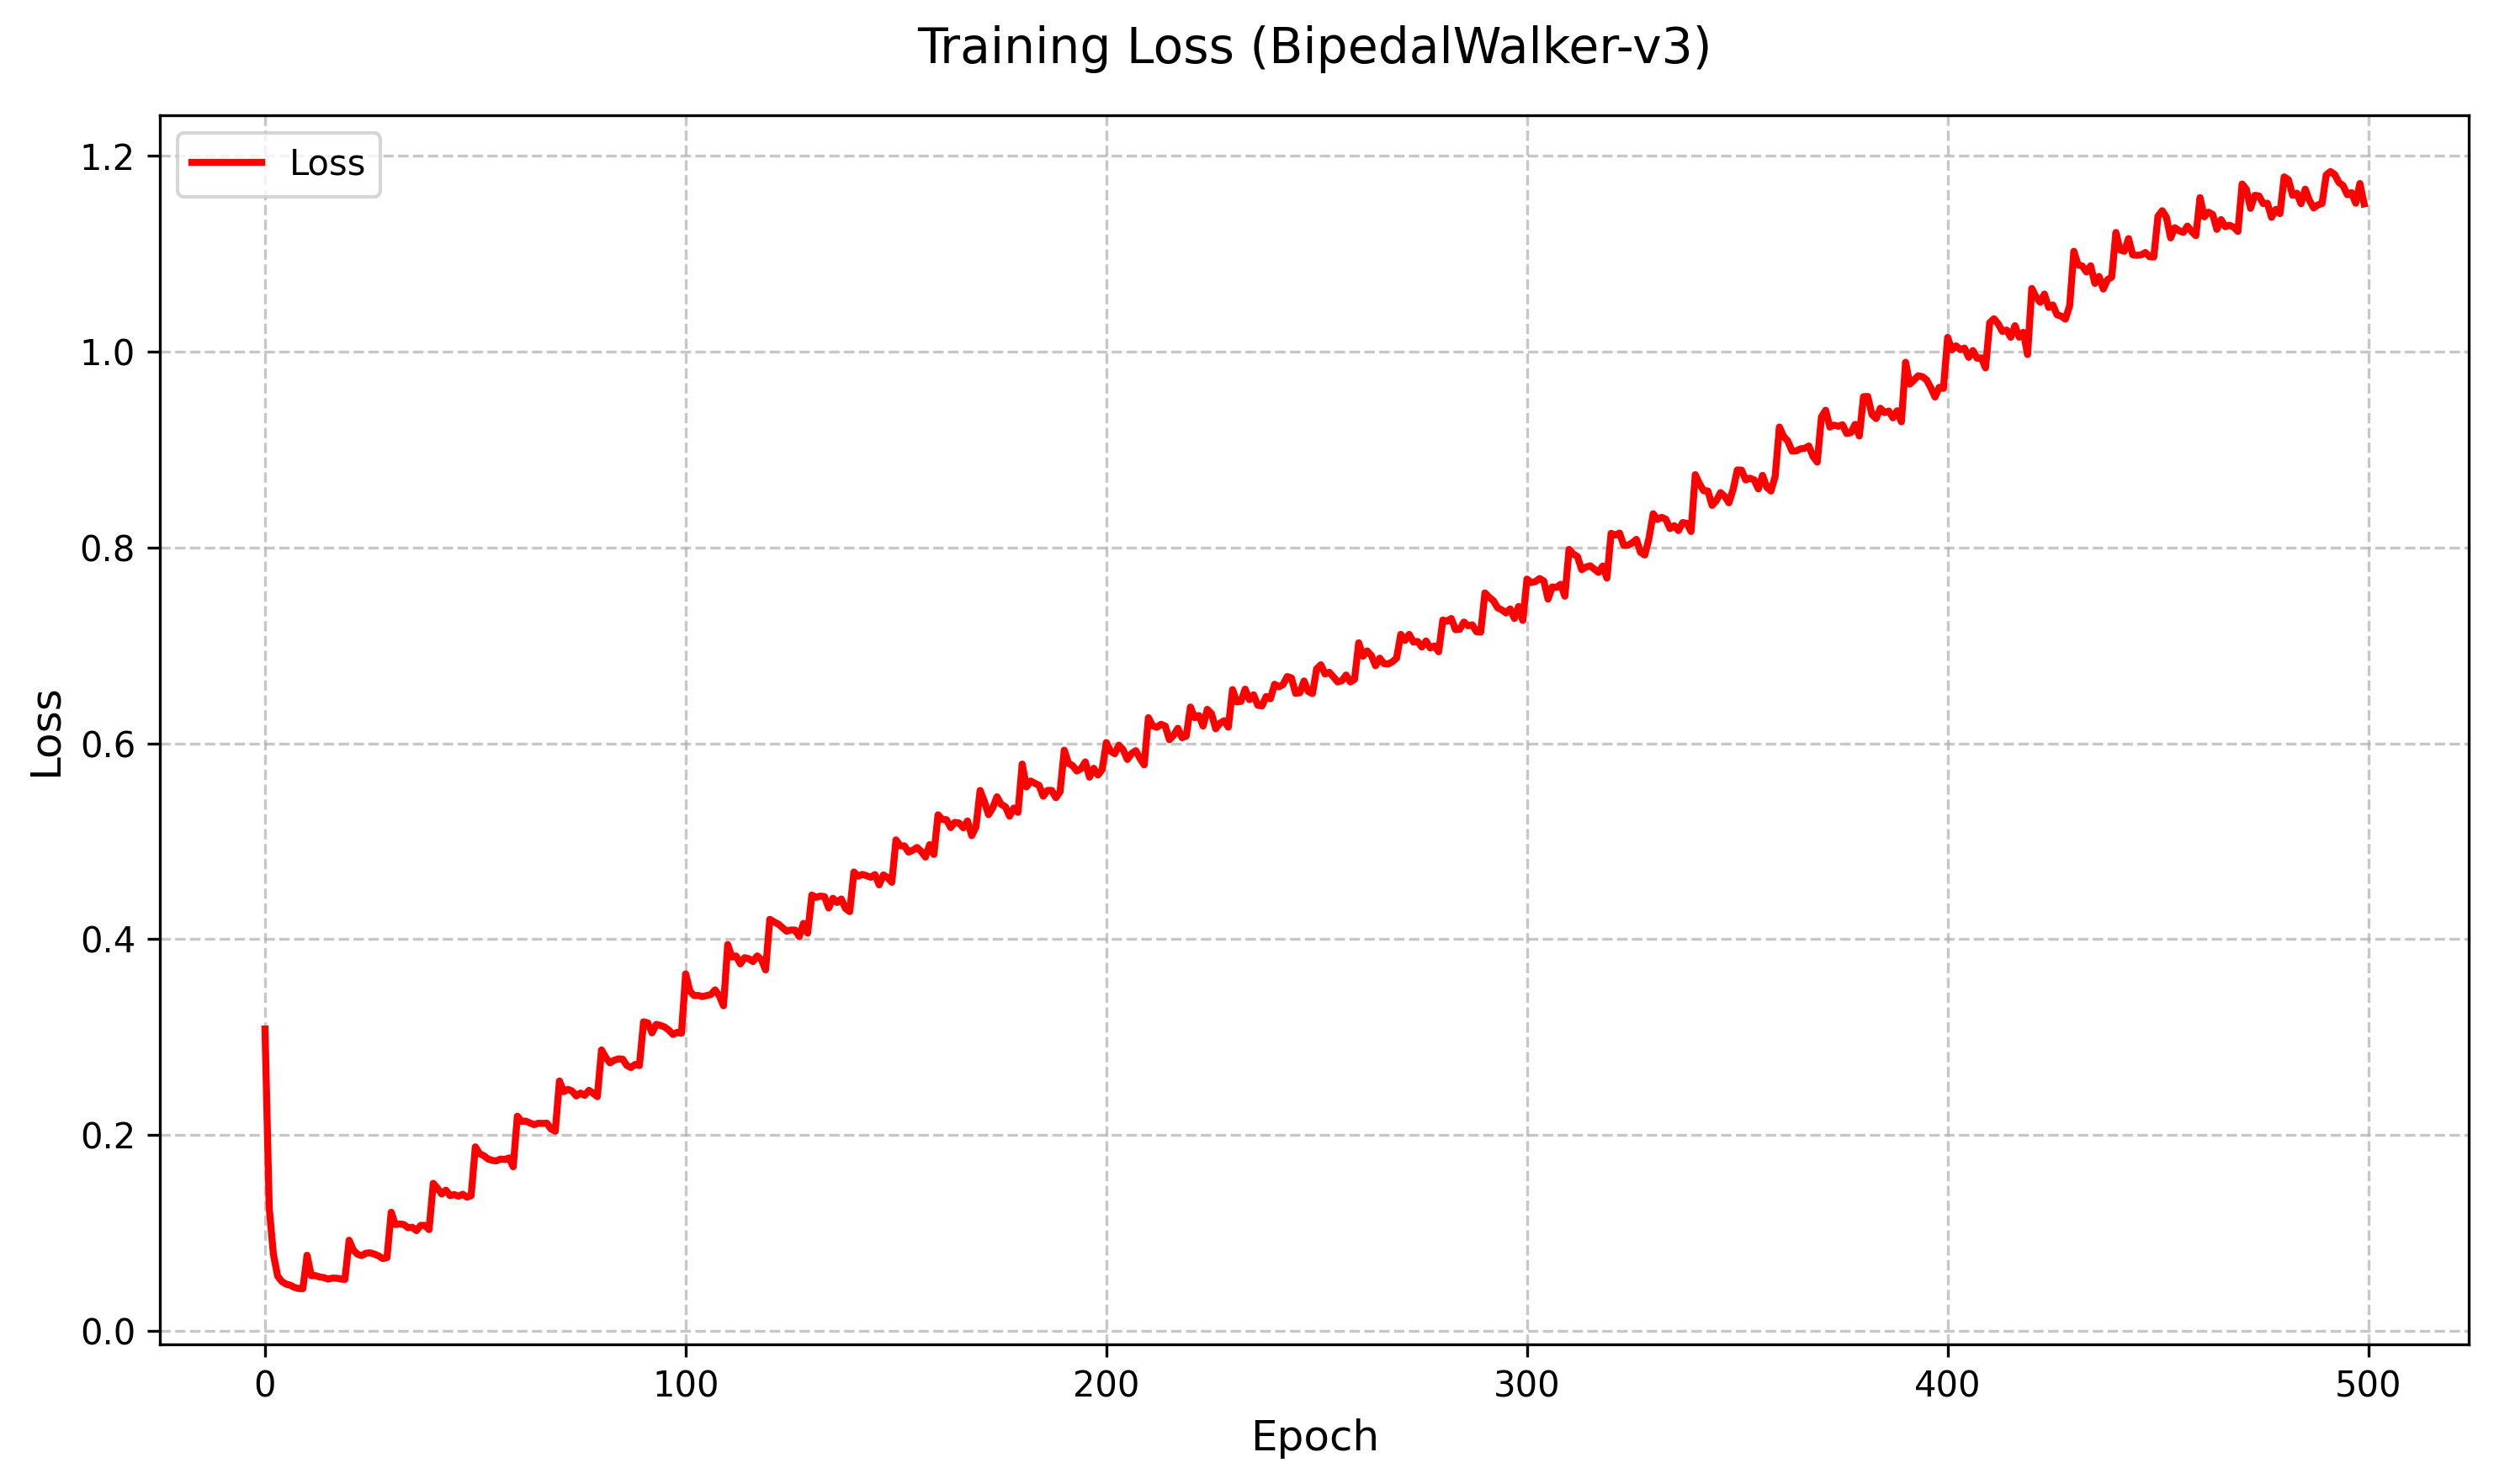
\includegraphics[width=\linewidth]{img/06-boltzmann--bw-boltzmann-final-01--loss.png}
        \caption{Loss}
    \end{subfigure}
    \caption{Category 06: Boltzmann Strategy Final vs. Baseline}
    \label{fig:cat06}
\end{figure}

% Hardcore comparison
\begin{figure}[H]
    \centering
    \begin{subfigure}{0.31\textwidth}
        \centering
        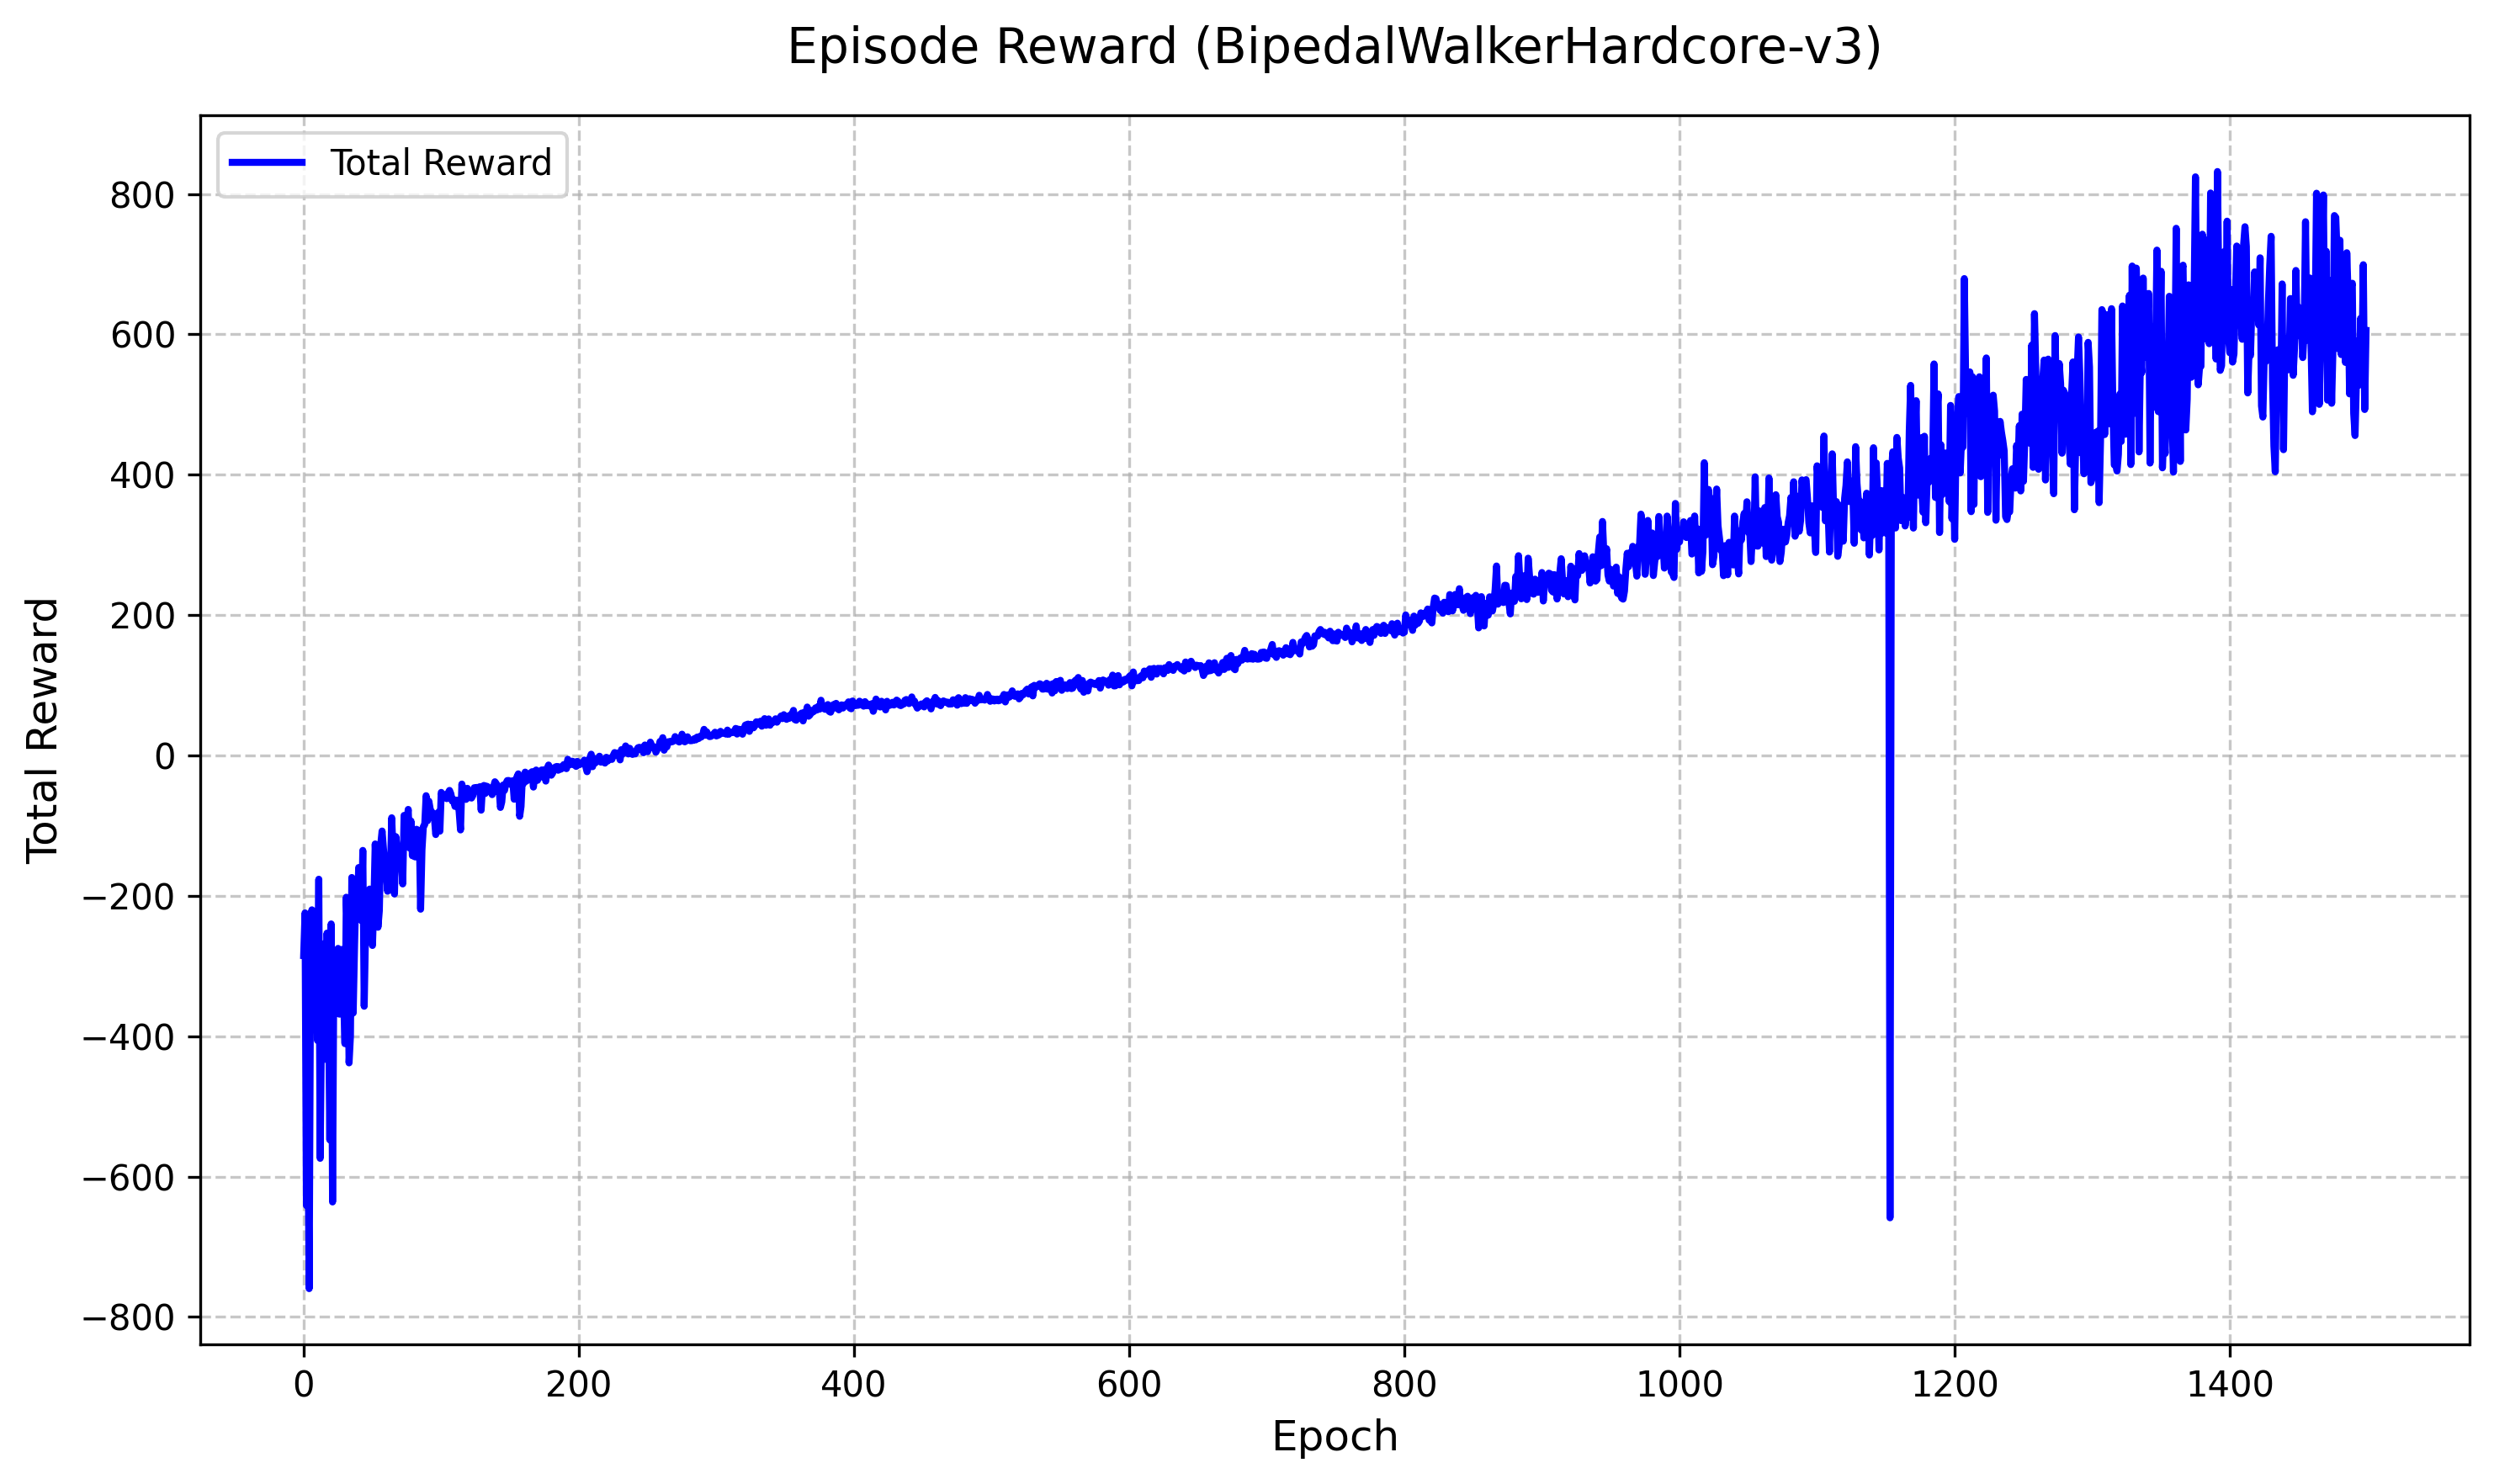
\includegraphics[width=\linewidth]{img/bwh-bw-reward.png}
        \caption{Reward}
    \end{subfigure}\hfill
    \begin{subfigure}{0.31\textwidth}
        \centering
        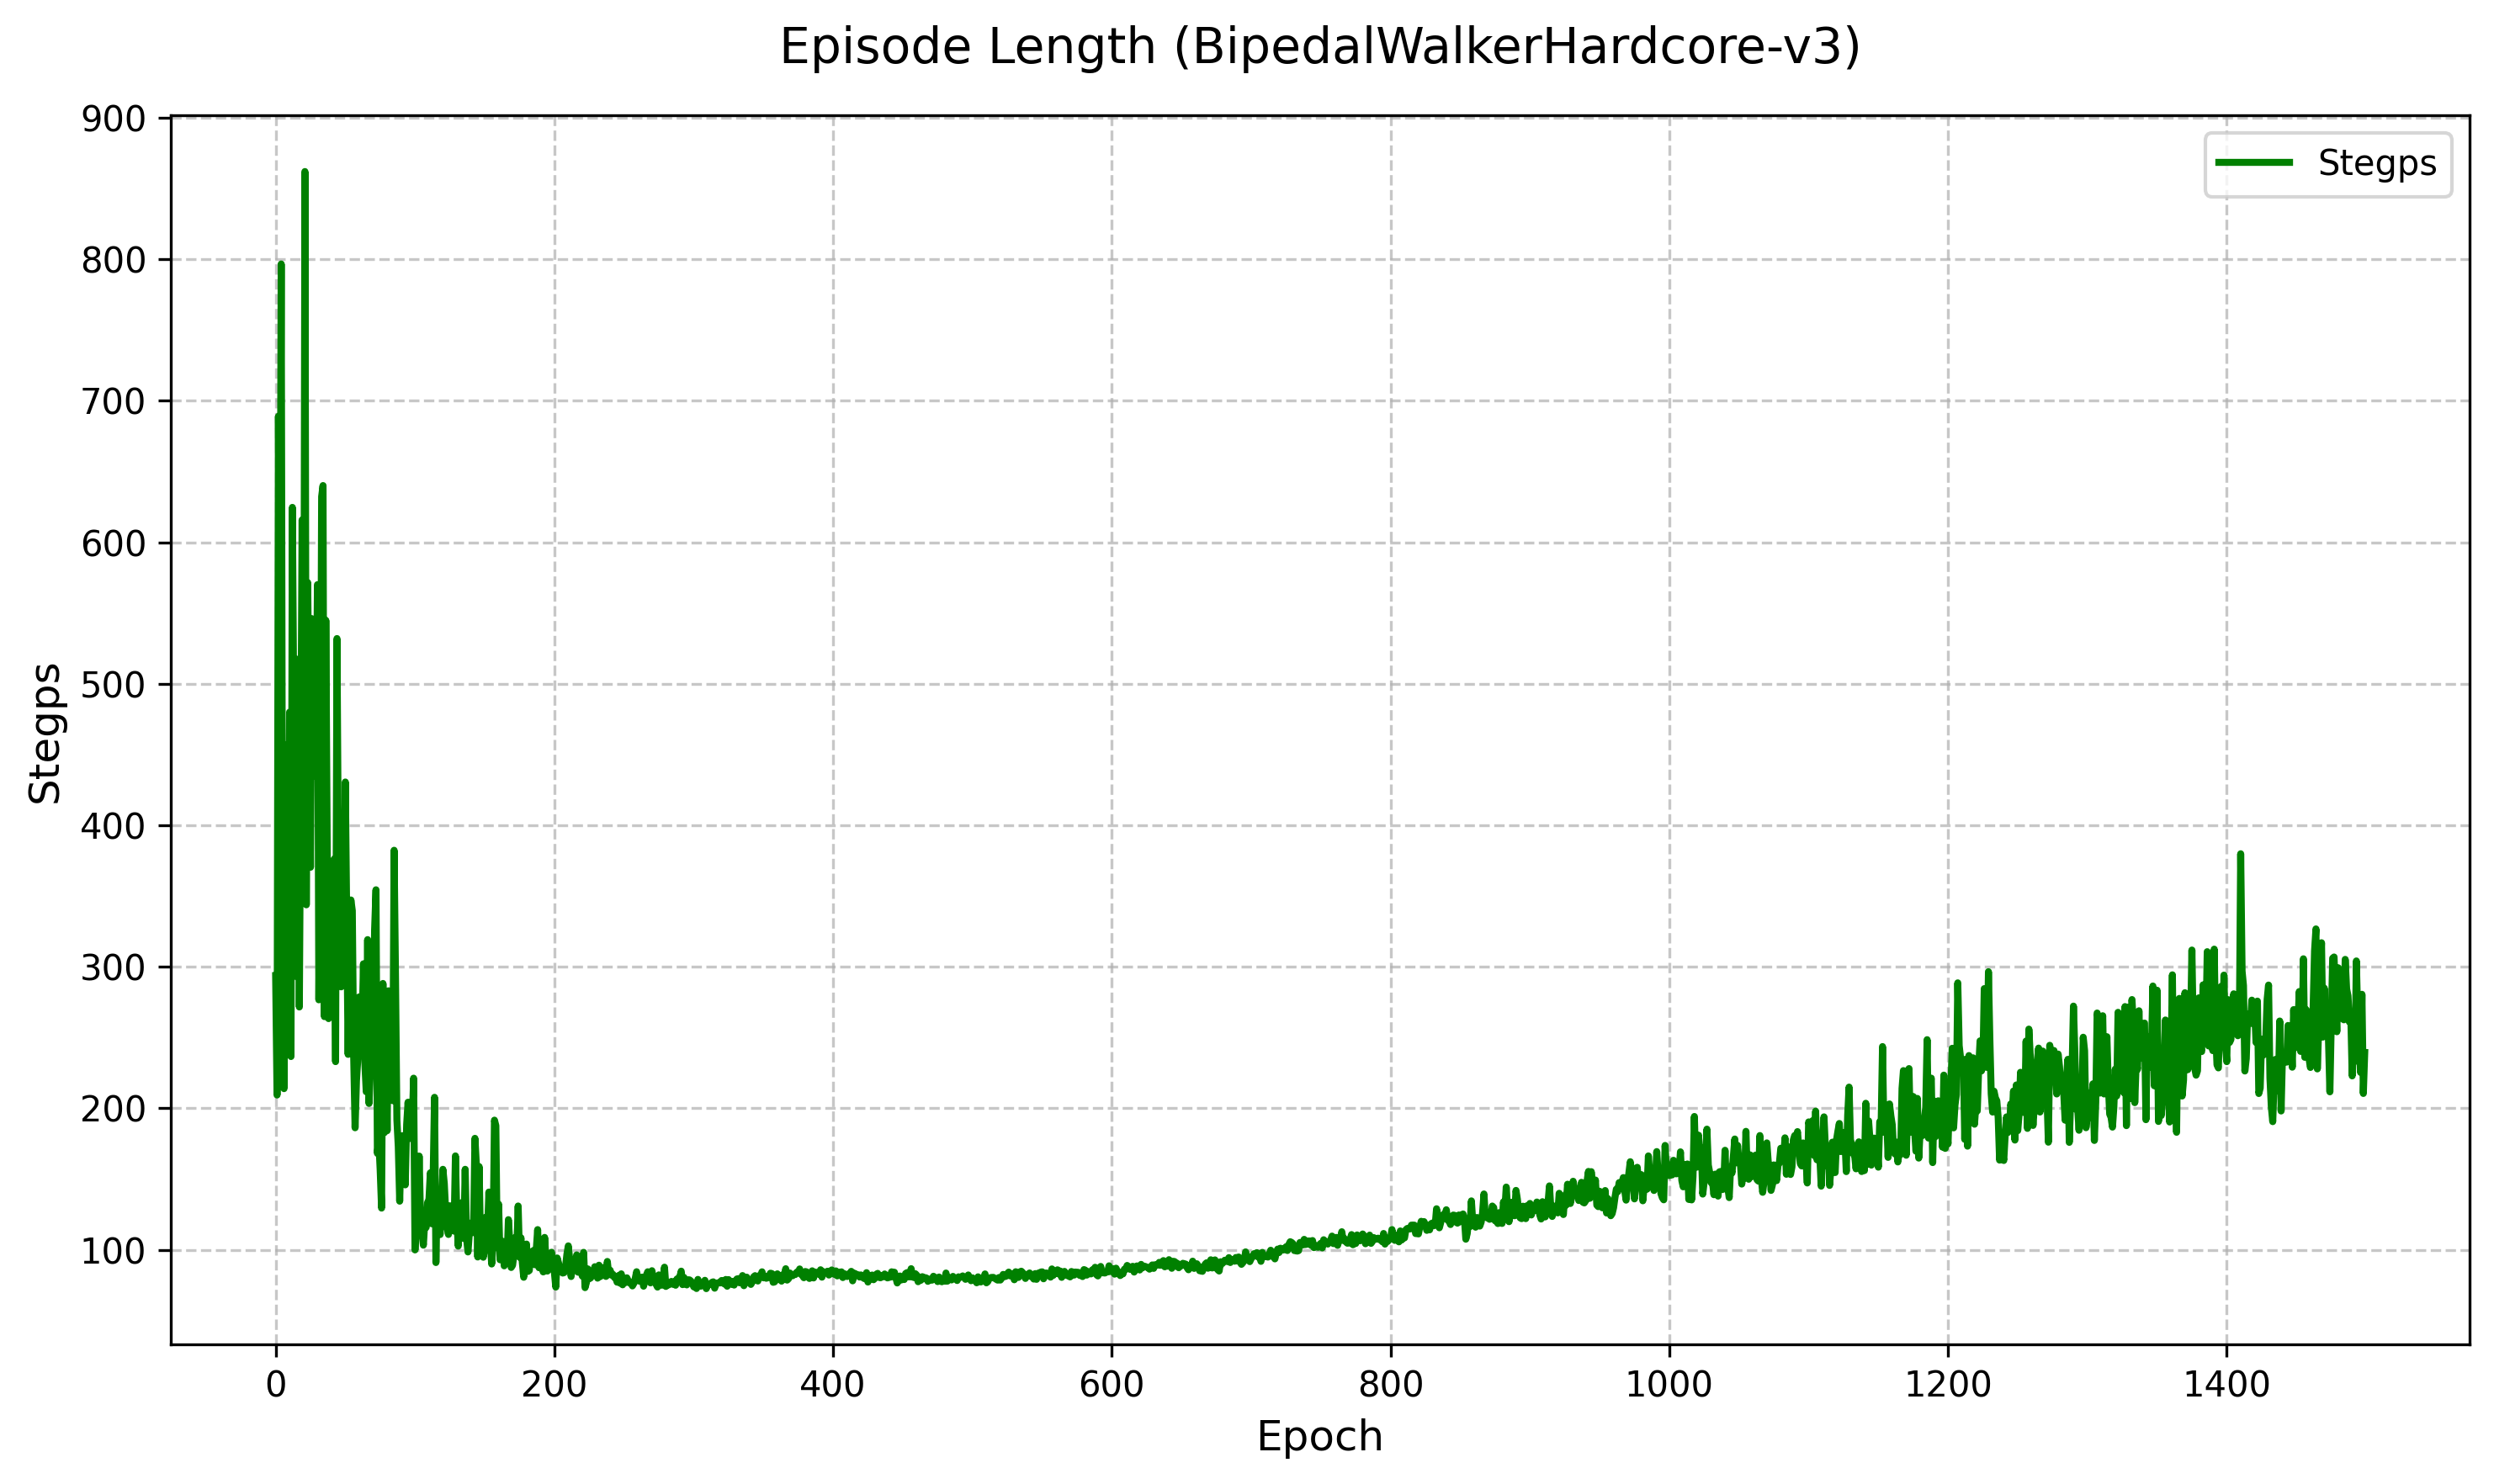
\includegraphics[width=\linewidth]{img/bwh-bw-length.png}
        \caption{Length}
    \end{subfigure}\hfill
    \begin{subfigure}{0.31\textwidth}
        \centering
        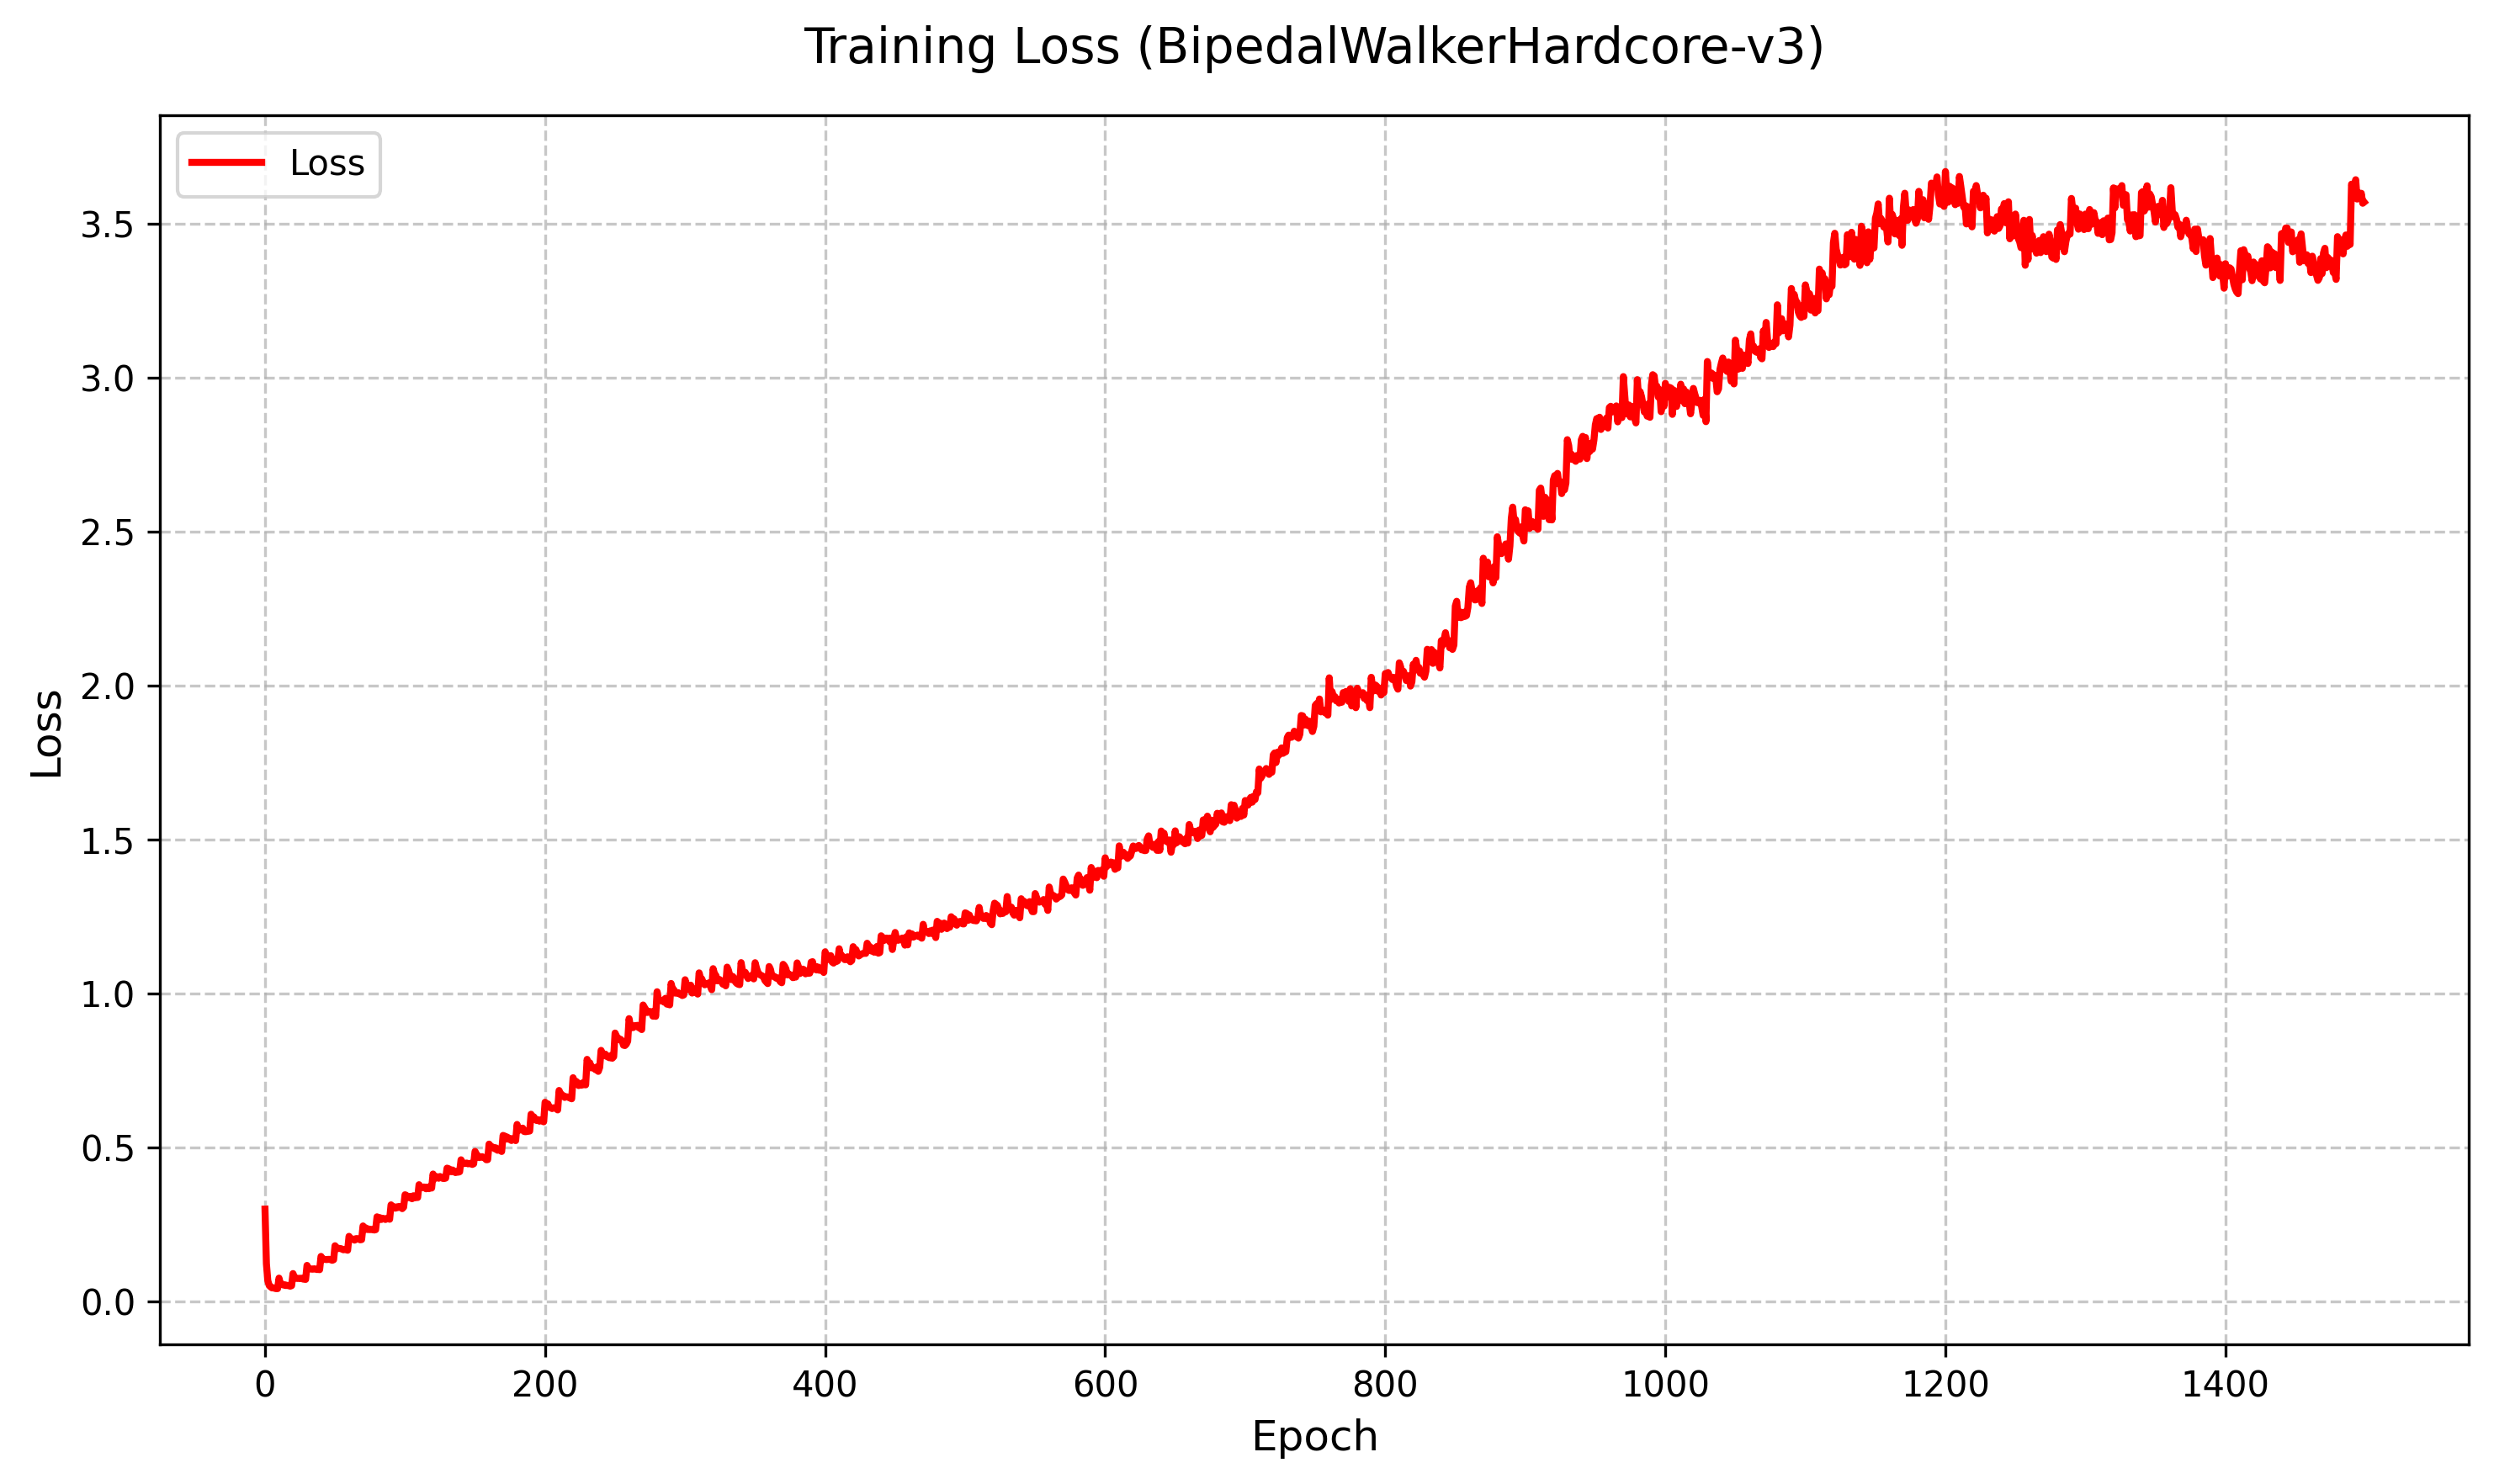
\includegraphics[width=\linewidth]{img/bwh-bw-loss.png}
        \caption{Loss}
    \end{subfigure}
    \caption{BipedalWalker default terrain vs. Hardcore terrain, using the same (default-tuned) hyperparameters. Episode length fails to increase on Hardcore, indicating that the agent does not learn to traverse the added obstacles.}
    \label{fig:hardcore}
\end{figure}
